\documentclass[12pt, oneside, numbers, spanish]{ezthesis}
%\usepackage[letterpaper,top=35mm,bottom=35mm,inner=30mm,outer=30mm]{geometry}
\usepackage[utf8x]{inputenc}
\usepackage{fancyhdr}
\usepackage[bottom]{footmisc}
\usepackage{graphicx}
\usepackage{tabularx}
\usepackage{pbox}
\usepackage[makeroom]{cancel}
\usepackage{float}
\usepackage{caption}
\usepackage{multirow}
\usepackage{newfloat}
\usepackage{gensymb}
\usepackage{array}
\usepackage{amssymb}
\usepackage{amsmath}
\usepackage{xcolor}
\usepackage{times}
\usepackage{tikz}
%\usepackage{dsfont}
%\usepackage{hyperref}
\DeclareFloatingEnvironment[name={Gráfico}]{graph}
%\numberwithin{graph}{section}
\newcommand\numberthis{\addtocounter{equation}{1}\tag{\theequation}}
\setcounter{MaxMatrixCols}{20}
\numberwithin{equation}{section}
%\numberwithin{figure}{section}


\date{\today}
\renewcommand{\contentsname}{Contenidos}
\renewcommand\refname{Referencias}
\renewcommand\tablename{Tabla}
\renewcommand\figurename{Figura}
\newcommand{\norm}[1]{\left\lVert#1\right\rVert}
\newcommand{\circled}[1]{\tikz[baseline=(char.base)]{\node[shape=circle,draw,inner sep=1pt] (char) {#1};}}
\newcommand\varpm{\mathbin{\vcenter{\hbox{\oalign{\hfil$\scriptstyle+$\hfil\cr\noalign{\kern-.3ex}$\scriptscriptstyle({-})$\cr}}}}}
\newcommand\varmp{\mathbin{\vcenter{\hbox{\oalign{$\scriptstyle({+})$\cr\noalign{\kern-.3ex}\hfil$\scriptscriptstyle-$\hfil\cr}}}}}
\newcommand\votwo{\mathbin{\vcenter{\hbox{\oalign{\hfil$\scriptstyle1$\hfil\cr\noalign{\kern-.3ex}$\scriptscriptstyle({2})$\cr}}}}}
\newcommand{\angstrom}{\text{\normalfont\AA}}
\renewcommand{\baselinestretch}{1.5}

\author{Nicolás Espinoza Muñoz}
\title{MODELACIÓN NUMÉRICA DE UNA PROTEÍNA INSERTA EN UNA MEMBRANA CELULAR USANDO EL MÉTODO DE ELEMENTOS DE BORDE.}
\supervisor{Christopher D. Cooper V. Ph.D.}
\correferent{Harvey A. Zambrano R. Ph.D.}
\institution{UNIVERSIDAD TÉCNICA FEDERICO SANTA MARÍA}
\department{DEPARTAMENTO DE INGENIERÍA MECÁNICA}
\city{VALPARAISO}
\country{CHILE}

\geometry{letterpaper,top=35mm,bottom=35mm,inner=30mm,outer=30mm}
%\geometry{top=35mm,bottom=35mm,inner=30mm,outer=30mm}

\begin{document}

%% ## Construye tu propia portada ##
%% 
%% Una portada se conforma por una secuencia de "Blocks" que incluyen
%% piezas individuales de informaci'on. Un "Block" puede incluir, por
%% ejemplo, el t'itulo del documento, una im'agen (logotipo de la universidad),
%% el nombre del autor, nombre del supervisor, u cualquier otra pieza de
%% informaci'on.
%%
%% Cada "Block" aparece centrado horizontalmente en la p'agina y,
%% verticalmente, todos los "Blocks" se distruyen de manera uniforme 
%% a lo largo de p'agina.
%%
%% Nota tambi'en que, dentro de un mismo "Block" se pueden cortar
%% lineas usando el comando \\
%%
%% El tama'no del texto dentro de un "Block" se puede modificar usando uno de
%% los comandos:
%%   \small      \LARGE
%%   \large      \huge
%%   \Large      \Huge
%%
%% Y el tipo de letra se puede modificar usando:
%%   \bfseries - negritas
%%   \itshape  - it'alicas
%%   \scshape  - small caps
%%   \slshape  - slanted
%%   \sffamily - sans serif
%%
%% Para producir plantillas generales, la informaci'on que ha sido inclu'ida
%% en el archivo principal "tesis.tex" se puede accesar aqu'i usando:
%%   \insertauthor
%%   \inserttitle
%%   \insertsupervisor
%%	 \insertcorreferent
%%   \insertinstitution
%%   \insertdegree
%%   \insertfaculty
%%   \insertdepartment
%%	 \insertcity
%%	 \insertcountry
%%   \insertsubmitdate

\begin{titlepage}
	\TitleBlock[\vspace{-1.5 in}]{
\includegraphics[height=4cm]{Imagenes/utfsm_logo}}
	\TitleBlock[\vspace{0.05in}]{\bfseries\insertinstitution}
	\TitleBlock[\vspace{0.05in}]{\insertdepartment}
	\TitleBlock[\vspace{0.05in}]{\insertcity  - \insertcountry}
	\TitleBlock[\vspace{1.2in}]{\Large\scshape\bfseries\inserttitle}
    \TitleBlock[\vspace{1.5in}]{\bfseries\insertauthor}
%	\TitleBlock[\vspace{0.1in}]{\insertdegree}
	\TitleBlock[\vspace{0.1in}]{Septiembre - \insertsubmitdate}
\end{titlepage}

%% Nota 1:
%% Se puede agregar un escudo o logotipo en un "Block" como:
%%   \TitleBlock{\includegraphics[height=4cm]{escudo_uni}}
%% y teniendo un archivo "escudo_uni.pdf", "escudo_uni.png" o "escudo_uni.jpg"
%% en alg'un lugar donde LaTeX lo pueda encontrar.

%% Nota 2:
%% Normalmente, el espacio entre "Blocks" se extiende de modo que el
%% contenido se reparte uniformemente sobre toda la p'agina. Este
%% comportamiento se puede modificar para mantener fijo, por ejemplo, el
%% espacio entre un par de "Blocks". Escribiendo:
%%   \TitleBlock{Bloque 1}
%%   \TitleBlock[\bigskip]{Bloque2}
%% se deja un espacio "grande" y de tama~no fijo entre el bloque 1 y 2.
%% Adem'as de \bigskip est'an tambi'en \smallskip y \medskip. Si necesitas
%% aun m'as control puedes usar tambi'en, por ejemplo, \vspace*{2cm}.




\newpage
%\noindent
%\\\\\\\\\\\\
%\large{``The greatest danger for most of us}
%\begin{center}
%\large{is not that our aim is too high and we miss it,}
%\end{center}
%\begin{flushright}
%\large{but that it is too low and we reach it."\\}
%\end{flushright}
%- Michelangelo
%\newpage
\tableofcontents
\newpage

\chapter{Introducción}\label{Chap:Intro}
En las últimas décadas ha crecido el interés por modelar de forma más precisa el comportamiento de sistemas biológicos, destacando las células y sus componentes y procesos. Es en esta línea de investigación que surgen y se desarrollan métodos para representar las interacciones que ocurren tanto dentro de la célula como a nivel extracelular.\\\\
Sin embargo, la complejidad de estos fenómenos hace que sea imposible hasta el momento abarcar de manera completa la naturaleza del proceso biológico correspondiente. Es por esto que actualmente se estudian de manera exhaustiva nuevas formas de representar los sistemas biológicos o sus elementos conformantes, recurriendo a múltiples disciplinas y enfoques. Por nombrar ejemplos de ramas de la ciencia relevantes se tienen la electrodinámica, la termodinámica, la mecánica de sólidos, y mecánica estadística, aunque de ninguna manera son las únicas. Además, al igual que en muchas otras áreas, la computación se tomó gran parte del escenario, volviéndose quizás la herramienta más útil y usada en las investigaciones y avances en la comprensión de la biología celular.\\\\
Para modelar la fenomenología de los sistemas biológicos según las diferentes disciplinas científicas mencionadas se utiliza una cantidad de métodos computacionales, de los cuales quizás los más conocidos son la dinámica molecular (MD) en casos explícitos y el método de elementos finitos (FEM) en casos implícitos. Por supuesto y como todo en la vida, ambos tienen sus ventajas y desventajas; un punto en contra que tienen en común ambos tipos de modelación es que en general son lentos. Por esto es que ha empezado a tomar cada vez más fuerza el método de elementos de borde/frontera (BEM), que permite resolver problemas físicos comparativamente rápido a expensas de una formulación un tanto más compleja.\\\\
El objetivo global de este trabajo consiste en obtener las ecuaciones de Green que permiten representar cargas en un medio acotado por dos interfaces paralelas, implementarlo en un programa de cálculo energético, y contrastar los resultados con aquellos de códigos o programas ya validados. Sumado a esto, la idea es que dicha implementación sea computacionalmente barata, conserve un buen nivel de precisión, y que la velocidad de cálculo sea competitiva frente a un programa de referencia en casos de estudio seleccionados. Hay que tener presente que existen otros fenómenos además de los electrostáticos que no se consideran por la gran complejidad que conllevan; por ejemplo, la inversión de carga de la membrana, la onda mecánica consecuente (o causal), etc, ya que en algunos casos ni siquiera se entiende bien su naturaleza; este trabajo se remite a electrostática de proteinas totalmente embebidas en la membrana.\\\\
El presente texto busca entonces \textit{presentar la física que ocurre tras una interacción electrostática en medios dieléctricos, trabajando un método que permita modelar una membrana celular a partir de un sistema de tres medios separados por dos interfaces, con cargas distribuidas en el medio encerrado. Teniendo este modelo, se lo implementa en un código y se procede a la comparación con programas ya reconocidos}.
%Sumado a esto se presentan resúmenes de publicaciones relevantes para la línea de estudio pertinente a este escrito, y que incluso podrían servir para mejorar la precisión del modelo al representar de manera más fiel la física de las interacciones de interés, al sumar otro tipo de interacciones o fenómenos, o al plantear respuestas a interrogantes que pudieran surgir en un futuro.\\\\
En primer lugar se presenta una introducción a la teoría que permite trabajar los sistemas dieléctricos con interfaz de forma macroscópica y mediante el método de imágenes. También se echa un vistazo a la formulación que da pie al método BEM, la denominada Boundary Integral Equation de un sistema de ecuaciones diferencial, además de contextualizar sobre aspectos básicos de la membrana para entender qué es lo que se busca. A continuación se presenta un ejemplo de formulación integral de frontera con el caso de la ecuación de Poisson - Boltzmann, que no se trabaja directamente en esta investigación, pero que va de la mano con la metodología de solvente implícito. Junto a esto, se describen los programas relevantes para este trabajo. Entrando a la parte fundamental de este trabajo, se desarrolla el método de imágenes para un sistema con dos interfaces paralelas, y cómo se incluye en la formulación, además de su implementación al programa \texttt{PyGBe}. Por último, se presentan los resultados obtenidos y cómo se comparan con los de programas como \texttt{APBS} y \texttt{APBSmem}; esto considera también la forma en que influye la variación de parámetros del método de imágenes en el resultado y los tiempos de cálculo. Tras tener estos resultados se termina presentando las conclusiones extraídas de este trabajo.


%%%%%%%%%%%%%%%%%%%%%%%%%%%%%%%%%%%%%%%%%%%%%%%%%%%%%


\chapter{Marco Teórico}\label{Chap:Teoria}
\section{El campo eléctrico y el potencial eléctrico}\label{Sec:E_field_Pot_elec}
El campo eléctrico correspondiente a una carga puntual $q$ que se encuentra en el vacío en la posición $\mathbf{r}_0$ viene dado por la conocida ecuación
\begin{equation}\label{eqn:charge_field}
\vec{E}(\mathbf{r}) = \frac{q}{4\pi\varepsilon_0}\frac{(\mathbf{r} - \mathbf{r}_0)}{|\mathbf{r}-\mathbf{r}_0|^3}
\end{equation}
siendo $\varepsilon_0$ la permitividad macroscópica del vacío, una medida de cómo fluye el campo eléctrico en el vacío. Por supuesto, en el caso ejemplificado en la Ec. (1), no hay un medio que reaccione, por lo que $\varepsilon_0$ es nuestra referencia. De ahora en adelante se trabaja con $\varepsilon$ propio de un dieléctrico; además se elabora más sobre la permitividad en la sección siguiente.\\\\
Cuando se cuenta con N cargas puntuales, la Ecuación (\ref{eqn:charge_field}) se convierte en una sumatoria sobre todos los elementos del sistema de cargas a considerar
\begin{equation}
\vec{E}(\mathbf{r}) = \sum_{j=1}^{N_q}\frac{q_j}{4\pi\varepsilon}\frac{(\mathbf{r} - \mathbf{r}_j)}{|\mathbf{r}-\mathbf{r}_j|^3}
\end{equation}
Para un caso con una distribución continua de carga, se define el flujo de campo eléctrico a través de una superficie que encierra toda la distribución de carga como
\begin{equation}
\int_{\partial\Omega}\vec{E}(\mathbf{r})\cdot \hat{\mathbf{n}}d\partial\Omega = \int_{\Omega} \frac{\rho}{\varepsilon} d\Omega \label{eqn:Gauss_law_int}
\end{equation}
Esta es la ley de Gauss en forma integral. Con el teorema de la divergencia aplicado a la Ec. (\ref{eqn:Gauss_law_int}) se llega a la ley de Gauss en forma diferencial:
\begin{equation}
\int_{\Omega} \nabla\cdot\vec{E} d\Omega = \int_\Omega \frac{\rho}{\varepsilon}d\Omega \implies \nabla\cdot\vec{E} = \frac{\rho}{\varepsilon} \label{eqn:Gauss_law_diff}
\end{equation}
Por otro lado, como el campo eléctrico es un campo vectorial irrotacional, se puede aplicar el teorema fundamental del cálculo para obtener su función potencial. Como $\vec{E}(\mathbf{r})$ es una variable solo de la diferencia de posiciones entre la de la carga y el punto de evaluación $|\mathbf{r} - \mathbf{r}_0|$ (función solo del radio), la integración es directa si la referencia para el potencial eléctrico se toma como $0$ al infinito, quedando
\begin{align*}\label{eqn:potential}
\vec{E} = \nabla\phi \quad\rightarrow\quad\phi{(\mathbf{r})} & = -\int_\infty^{\mathbf{r}} \vec{E}(\mathbf{r}^*) d\mathbf{r}^* \\
& = -\int_\infty^{\mathbf{r}} \frac{q}{4\pi\varepsilon}\frac{(\mathbf{r}^*-\mathbf{r}_0)}{|\mathbf{r}^* - \mathbf{r}_0|^3} d\mathbf{r}^* = \frac{q}{4\pi\varepsilon}\frac{1}{|\mathbf{r} - \mathbf{r}_0|}\numberthis
\end{align*}
Esto es en los casos en que se tenga una carga puntual, como en el caso de la Ec. (\ref{eqn:charge_field}). Para una carga distribuida se debe considerar la Ec. (\ref{eqn:Gauss_law_int}), lo que nos lleva a
\begin{equation}\label{eqn:integral_potential}
\phi(\mathbf{r}) = \int_\Omega \frac{\rho(\mathbf{r}_0)}{4\pi\varepsilon}\frac{1}{|\mathbf{r}-\mathbf{r}_0|}d\Omega
\end{equation}
En los casos en que el medio en el que está la carga $q$ no sea el vacío, se debe considerar que la materia que lo compone si reaccionará al campo eléctrico asociado a $q$; en estos casos, $\varepsilon \neq \varepsilon_0$. Es decir, hay que aclarar que las Ecs. (\ref{eqn:Gauss_law_int}) y (\ref{eqn:Gauss_law_diff}) no están completas, pues falta considerar el efecto de la \textit{polarización}. Además resulta interesante entender qué es realmente la permitividad, que esta relacionada directamente con la polarización del medio; a continuación se explican estos puntos.
\section{La permitividad de un medio material, la polarización y el campo eléctrico microscópico}\label{Sec:perm_polarization_mic_E_field}
Se puede entender la constante dieléctrica de un material (o permitividad) como una medida del reordenamiento de las partículas de un medio a nivel molecular frente a la presencia de un campo eléctrico externo y provocando así que dichas partículas generen un \textit{campo eléctrico inducido}, que es opuesto en sentido al original, pero no necesariamente de la misma intensidad; este disminuye el flujo neto del campo eléctrico externo, por lo que impide en cierta medida su paso, dando su nombre a la propiedad - en qué grado las moléculas del material \textbf{permiten} el flujo de campo eléctrico.\\\\
La permitividad que se utiliza en las Ecuaciones (\ref{eqn:charge_field} - \ref{eqn:integral_potential}) es llamada también \textit{constante dieléctrica} del medio, y en realidad es un concepto derivado de la susceptibilidad eléctrica y de lo que ocurre a nivel molecular en el medio dieléctrico afectado por un campo eléctrico. En el caso del vacío se menciona que no existe un medio que reaccione a la presencia de una carga (y por ende no ``siente" el campo eléctrico), por lo que la constante dieléctrica del vacío es considerada como referencia. Por el contrario, en un dieléctrico si se tiene una reacción al campo eléctrico; en este caso es importante explicar qué pasa con el campo eléctrico a nivel microscópico y cómo eso se relaciona con la susceptibilidad eléctrica. Los términos microscópico y local se utilizan indistintamente \cite{Kantorovich}.

\subsection{Campo eléctrico local, y polarización}\label{subsec:Local_Field}
\begin{figure}[H]
\centering
\input{./Figures/Fig_1.eps_tex}
\caption{Efecto de un campo sobre la forma de un átomo. El electrón (en realidad la nube electrónica) es ``halado" por el campo, mientras que el protón (o núcleo atómico) es ``empujado", induciendo así un dipolo.}
\label{fig:Polarization}
\end{figure}
Cuando se aplica un campo eléctrico externo a un cuerpo o medio (macroscópico) dieléctrico, las partículas constituyentes de los átomos se comportan de forma especial. Por ejemplo, en la Figura \ref{fig:Polarization} se muestra un átomo simple de hidrógeno que se reordena bajo la acción de un campo externo que rompe el equilibrio eléctrico del átomo, generando así un campo eléctrico opuesto con líneas de campo (inducido) que van del protón hacia el electrón (se representa la nube electrónica con un solo electrón por simplicidad). Este efecto es la polarización, e induce un momento dipolar $\mathbf{p}$ en los átomos afectados por el campo eléctrico a nivel local.
\begin{equation}
\mathbf{p} = \alpha\vec{E}^{loc}
\end{equation}
$\alpha$ se conoce como la polarizabilidad microscópica, un coeficiente de proporcionalidad que representa qué tanto se polariza la especie analizada - la magnitud del momento dipolar inducido - en presencia de un cierto campo eléctrico local $\vec{E}^{loc}$. Por supuesto, esta es una relación constitutiva, porque $\alpha$ depende del material o elemento estudiado. Ahora se hace la distinción entre los distintos campos eléctricos de interés para este apartado:
\begin{gather*}
\vec{E}^{ext} \quad \longrightarrow \quad \text{Campo eléctrico externo}\\
\vec{E}^{loc} \quad \longrightarrow \quad \text{Campo eléctrico local}\\
\vec{E}^{ind} \quad \longrightarrow \quad \text{Campo eléctrico inducido (microscópico)}\\
\vec{E} \quad \longrightarrow \quad \text{Campo eléctrico macroscópico}
\end{gather*}
y se define la relación entre los primeros tres como
\begin{equation}
\vec{E}^{loc} = \vec{E}^{ind} + \vec{E}^{ext}
\end{equation}
Es conveniente explicar que si bien se define uno de los campos como microscópico o local, esto no es el campo debido a un único átomo o molécula, sino el propio de un volumen macroscópicamente pequeño pero microscópicamente grande; por lo tanto, los términos local y microscópico son en realidad promedios sobre volúmenes más pequeños que el campo de las ecuaciones de Maxwell. Hay que notar también que si el campo eléctrico se transmite por el vacío, $\vec{E}^{ind} = 0$, y por ende $\vec{E}^{ext} = \vec{E}^{loc} = \vec{E}$. No se entra en detalle respecto al álgebra pues existen referencias sobre el tema, como por ejemplo el texto de Kantorovich \cite{Kantorovich}, pero después de algo de trabajo se llega a la expresión para el campo eléctrico local, también llamado campo de Lorentz, en función del campo macroscópico
\begin{equation}
\vec{E}^{loc} = \vec{E}(1 + \kappa)\label{eqn:Local_Field}
\end{equation}
donde $\kappa$ es un factor de corrección que depende del ordenamiento microscópico. El campo eléctrico local es el campo que siente cada uno de los muchos volúmenes pequeños que, en conjunto, componen el medio macroscópico que estamos estudiando. Por último se presenta la definición de densidad de polarización $\vec{P}$ para cerrar el círculo de relaciones entre el dieléctrico estudiado a nivel macroscópico y microscópico. La densidad de polarización por unidad de volumen se define de dos maneras; esto sale de diversas fuentes, pero W. Cai \cite{Cai} lo resume todo de forma simple:
\begin{gather}
\vec{P}(\mathbf{r}) = \sum_i N_i\alpha_i\left[\vec{E}(\mathbf{r})^{loc}\right]_i = \sum_i N_i\mathbf{p}_i\label{eqn:Micro_Polarization_sumation}\\
\vec{P}(\mathbf{r}) = \varepsilon_0\chi\vec{E}(\mathbf{r})\label{eqn:Macro_Polarization}
\end{gather}
con $N_i$ la densidad numérica (\textit{number density}) del $i$-ésimo átomo por unidad de volumen, y $\chi$ la susceptibilidad del medio dieléctrico (que en el caso del vacío es 0). Antes de continuar el desarrollo, se procede a definir qué son la densidad de polarización y la susceptibilidad. Como concepto, la densidad de polarización es la polarización a nivel macroscópico, por unidad de volumen, causada por todos los momentos dipolares inducidos en las moléculas de dicho volumen asociados al campo eléctrico que los induce. Por otra parte, la susceptibilidad permite relacionar un campo eléctrico macroscópico con los efectos que este tiene en el momento dipolar de las partículas en un volumen a través de la densidad de polarización, como se indica en la Ec. \ref{eqn:Macro_Polarization}; más allá de ser una constante de proporcionalidad, la susceptibilidad indica de forma promediada cómo influye el campo eléctrico en la orientación de los dipolos, y cómo varía el momentum dipolar del medio a nivel macroscópico en presencia del campo eléctrico. Hay que resaltar que esto no implica traslación o \textit{migración} electrónica, sino solo rotación del átomo o molécula para la reorientación del dipolo, intentando alinearlo con el campo.\\\\
Para terminar esta parte del desarrollo teórico, de las Ecs. (\ref{eqn:Local_Field} - \ref{eqn:Macro_Polarization}) y sabiendo que el campo macroscópico es el mismo, se puede deducir que
\begin{equation}
\vec{P}(\mathbf{r}) = \varepsilon_0\chi\vec{E}(\mathbf{r}) = \vec{E}(\mathbf{r})\sum_iN_i\alpha_i(1+\kappa_i) \implies \varepsilon_0\chi = \sum_iN_i\alpha_i(1+\kappa_i)
\end{equation}
Un caso particular es la teoría de Clausius-Mossotti. Aquí el valor de $\kappa_i = \kappa$ es $\chi/3$; uno de los supuestos es que la distribución molecular es una malla cúbica regular.\\\\
Con esto se puede entender de manera general cómo se relacionan el campo eléctrico macroscópico y microscópico. El propósito de este apartado es simplemente aclarar que ambos análisis no son independientes y que el tratamiento de continuo que se dará en lo sucesivo esta fundamentado en teoría del comportamiento eléctrico molecular; es por esto que se omiten pasos y solo se presentan resultados que se consideran importantes.

\subsection{Permitividad de un medio macroscópico}\label{subsec:Macro_perm}
Ya se explicó qué son la susceptibilidad y densidad de polarización, por lo que se procede a definir un poco mejor qué es la permitividad, profundizando en lo que se mencionó al principio de la Sección \ref{Sec:perm_polarization_mic_E_field}.
%\begin{figure}
%\centering
%\includegraphics[scale=]{•}
%\caption{}
%\end{figure}
Primero corresponde aclarar que la permitividad es netamente una propiedad macroscópica del medio, pero se prefiere caer en la redundancia un par de veces, como en el caso del título de esta sección, para reafirmar este punto. Cuando un campo eléctrico afecta un medio dieléctrico, los dipolos no solo se intentan alinear con las líneas de campo, sino que además hay un \textit{movimiento de cargas libres} dentro del cuerpo. Sumado a esto está el hecho de que los átomos conformantes del medio rompen el estado de equilibrio, pues los protones son repelidos por el campo, mientras que los electrones son atraidos por este (Fig. \ref{fig:Polarization}). Dicho efecto genera que se formen nuevos dipolos y en consecuencia que haya un momento dipolar distinto al original en el medio; es por esta razón que la susceptibilidad se relaciona con la permitividad. Teniendo presentes los fenómenos recién nombrados, se reitera la definición de permitividad o constante dieléctrica como una cuantificación macroscópica promedio de la tendencia de un medio (en este caso un dieléctrico) a oponerse al flujo de campo eléctrico por alguno de los mecanismos nombrados anteriormente.\\\\
Existen tres \textit{permitividades} de interés para este desarrollo: la permitividad del vacío $\varepsilon_0$, la permitividad propia de un material $\varepsilon$, y la permitividad relativa o constante dieléctrica, a la que en este caso se da más importancia
\begin{equation}\label{eqn:Permittivity_definition}
\varepsilon_r = \frac{\varepsilon}{\varepsilon_0}=\varepsilon_0(1+\chi)
\end{equation}
(llamada $k$ en algunas fuentes). De ahora en adelante, $\varepsilon$ a secas pasa a ser la permitividad relativa y se denomina simplemente \textit{permitividad} o \textit{constante dieléctrica} de un medio.\footnote{En estricto rigor, la constante dieléctrica es $\varepsilon_r\cdot\varepsilon_0$, pero por costumbre se utiliza este término para referirse a la propiedad adimensional en este informe.}
\section{Desplazamiento eléctrico y campo eléctrico en un dieléctrico}\label{Sec:Elec_Displacement}
En lo sucesivo, todo el trabajo es relativo a un medio o campo macroscópico. En este informe no se trabaja directamente con los momentos dipolares, la susceptibilidad, o incluso con la densidad de polarización, sino que se presenta una sola ecuación que engloba todos los efectos de un campo eléctrico sobre un dieléctrico; para llegar a dicha ecuación se utilizan las relaciones ya introducidas y un par de definiciones nuevas.\\\\
La Ec. (\ref{eqn:Macro_Polarization}) es una expresión que asocia el campo eléctrico y la densidad de polarización, establecida a través de la susceptibilidad y la permitividad. Además, la Ecuación (\ref{eqn:Gauss_law_int}) es la ley de Gauss para una distribución de carga, que tiene que ver únicamente con la permitividad.\\\\
Si se asume que el flujo de campo eléctrico se debe a contribuciones de la distribución de carga y de la polarización del medio únicamente, entonces se puede expresar dicho flujo de campo eléctrico como
\begin{equation}\label{eqn:Field_pol_rho_relation}
\nabla\cdot\vec{E} = \frac{\rho - \nabla\cdot\vec{P}}{\varepsilon_0}
\end{equation}
Se define entonces el \textit{desplazamiento eléctrico} como
\begin{equation}\label{eqn:Electric_Displacement}
\vec{D} = \vec{E} + \vec{P} = \varepsilon_0\vec{E}(1 + \chi)
\end{equation}
lo que nos permite escribir la Ec. (\ref{eqn:Field_pol_rho_relation}) como
\begin{equation}
\nabla\cdot\vec{D} = \rho
\end{equation}
Esto corresponde al efecto completo del flujo de campo eléctrico sobre el medio. En general, en la Ec.(\ref{eqn:Electric_Displacement}) se asocia el campo eléctrico $\vec{E}$ a las cargas libres (free charges) y la densidad de polarización $\vec{P}$ a las cargas fijas (bound charges), pero para el objetivo de este texto eso no es relevante.\\\\
Siguiendo con la idea, recordando que ahora $\varepsilon_r = \varepsilon$ y suponiendo que la permitividad es una propiedad isotrópica, y usando la Ec. (\ref{eqn:Permittivity_definition}) en la (\ref{eqn:Electric_Displacement}), se puede obtener
\begin{equation}
\vec{D} = \varepsilon\vec{E}\quad\biggm/\nabla\cdot\qquad\rightarrow\qquad\nabla\cdot\vec{D}=\nabla\cdot(\varepsilon\vec{E}) = \nabla(\varepsilon)\cdot\vec{E} + \varepsilon\nabla\cdot\vec{E} = \rho
\end{equation}
Aún más, si la permitividad del medio es constante sobre el mismo, entonces el término $\nabla (\varepsilon)\cdot\vec{E}$ se anula.\\\\
Es así que se retorna a la ecuación de la que prácticamente parte el desarrollo de la teoría, la ley de Gauss.
\begin{equation}
\nabla\cdot\vec{E} = \frac{\rho}{\varepsilon}
\end{equation}
El gran progreso es haber demostrado que (\ref{eqn:Gauss_law_diff}) no solo sirve para calcular el campo eléctrico en el vacío, sino que se puede aplicar a los dieléctricos en general y que incluso se consideran los efectos de polarización inducidos.

\section{Método de imágenes}\label{Sec:Image_Method}
En la teoría electrostática hay ocasiones en que hay que trabajar con interfaces que separan distintos medios dieléctricos. El método de imágenes destaca por su simpleza en este tipo de escenarios. La idea es que cargas en un medio inducirán un campo opuesto en el otro, el denominado campo de reacción. A su vez este campo inducido afectará al campo en el primer medio, por lo que hay que encontrar una expresión para el comportamiento de los campos eléctricos en los dos medios; por supuesto, este problema no se soluciona simplemente con aplicar la Ec. (\ref{eqn:charge_field}).\\\\
El método de imágenes facilita la resolución del problema de una forma simple: En vez de considerar la polarización y el consecuente campo inducido por el segundo medio como un todo, se hace más fácil poner una carga o distribución de cargas imágenes (puede ser incluso una distribución continua) de tal forma que el efecto de dicha carga sobre el primer medio sea el mismo que si hubiera un campo de reacción. Para esto uno analiza los distintos medios por separado en vez de como un sistema.\\\\
Como la interfaz es un límite para el espacio de análisis, es aquí donde se establecen las condiciones de frontera. Para un sistema de coordenadas adecuado al problema, existen condiciones para la componente normal del campo y para su componente tangencial justo en la interfaz. Matemáticamente esto es
\begin{gather}
\varepsilon_1\vec{E}_1\cdot\hat{\mathbf{n}} = \varepsilon_2\vec{E}_2\cdot\hat{\mathbf{n}} \label{eqn:jump_condition}\\
\vec{E}_1\cdot\hat{\mathbf{t}} = \vec{E}_2\cdot\hat{\mathbf{t}} \label{eqn:pot_continuity}
\end{gather}
En este caso, $\hat{\mathbf{n}}$ es un vector normal a la superficie interfaz, y $\hat{\mathbf{t}}$ un vector tangencial a la misma. En palabras, las Ecs. (20) y (21) nos indican que hay un cambio en la componente normal del campo igual a $\varepsilon_1/\varepsilon_2$; esto es, hay un salto en la componente normal. Como ejemplo se tiene el caso más simple, con dos dieléctricos homogéneos isotrópicos ($\varepsilon = cte$) en la Figura 2. Hay que notar que, como se dijo, al trabajar de esta forma se analizan los medios por separado, y se debe considerar el efecto de la carga imagen que representa el campo de reacción solo en el medio 1.
\begin{figure}[H]
\vspace{2cm}
\centering
%LaTeX with PSTricks extensions
%%Creator: inkscape 0.91
%%Please note this file requires PSTricks extensions
\psset{xunit=.5pt,yunit=.5pt,runit=.5pt}
\begin{pspicture}(250,300)
{
\newrgbcolor{curcolor}{0 0 0}
\pscustom[linewidth=1.35988307,linecolor=curcolor]
{
\newpath
\moveto(104.57652,191.37501)
\lineto(104.57652,68.98554)
}
}
{
\newrgbcolor{curcolor}{0 0 0}
\pscustom[linestyle=none,fillstyle=solid,fillcolor=curcolor]
{
\newpath
\moveto(49.50125837,130.18027523)
\curveto(49.50125837,126.42506196)(46.45705653,123.38086012)(42.70184326,123.38086012)
\curveto(38.94662999,123.38086012)(35.90242815,126.42506196)(35.90242815,130.18027523)
\curveto(35.90242815,133.93548851)(38.94662999,136.97969035)(42.70184326,136.97969035)
\curveto(46.45705653,136.97969035)(49.50125837,133.93548851)(49.50125837,130.18027523)
\closepath
}
}
{
\newrgbcolor{curcolor}{0 0 0}
\pscustom[linestyle=none,fillstyle=solid,fillcolor=curcolor]
{
\newpath
\moveto(185.48957014,130.18027523)
\curveto(185.48957014,126.42506196)(182.4453683,123.38086012)(178.69015503,123.38086012)
\curveto(174.93494176,123.38086012)(171.89073992,126.42506196)(171.89073992,130.18027523)
\curveto(171.89073992,133.93548851)(174.93494176,136.97969035)(178.69015503,136.97969035)
\curveto(182.4453683,136.97969035)(185.48957014,133.93548851)(185.48957014,130.18027523)
\closepath
}
}
{
\newrgbcolor{curcolor}{0 0 0}
\pscustom[linestyle=none,fillstyle=solid,fillcolor=curcolor]
{
\newpath
\moveto(35.39551906,231.08244852)
\lineto(34.0675083,231.08244852)
\lineto(34.05422819,235.07976092)
\curveto(33.12462066,235.09746773)(32.19501313,235.20370859)(31.26540559,235.3984835)
\curveto(30.33579806,235.60211182)(29.40176383,235.90312759)(28.46330289,236.30153082)
\lineto(28.46330289,238.69195019)
\curveto(29.36635021,238.12533226)(30.27825093,237.69594212)(31.19900506,237.40377975)
\curveto(32.12861259,237.12047079)(33.08478034,236.9743896)(34.0675083,236.9655362)
\lineto(34.0675083,243.02126527)
\curveto(32.11090578,243.33998785)(30.68550756,243.88004556)(29.79131365,244.6414384)
\curveto(28.90597314,245.40283124)(28.46330289,246.44753304)(28.46330289,247.7755438)
\curveto(28.46330289,249.21864883)(28.94581346,250.35631138)(29.91083462,251.18853146)
\curveto(30.87585577,252.02075153)(32.26141367,252.49883541)(34.0675083,252.62278308)
\lineto(34.0675083,255.74360837)
\lineto(35.39551906,255.74360837)
\lineto(35.39551906,252.6626234)
\curveto(36.21888574,252.62720978)(37.01569219,252.53867573)(37.78593843,252.39702125)
\curveto(38.55618468,252.26422017)(39.30872411,252.07829867)(40.04355673,251.83925673)
\lineto(40.04355673,249.5152379)
\curveto(39.30872411,249.88708091)(38.55175797,250.17481657)(37.77265833,250.37844489)
\curveto(37.00241209,250.58207321)(36.21003233,250.70159418)(35.39551906,250.7370078)
\lineto(35.39551906,245.06640184)
\curveto(37.40524202,244.75653267)(38.88376066,244.20319485)(39.83107501,243.40638839)
\curveto(40.77838935,242.60958193)(41.25204652,241.52061311)(41.25204652,240.13948192)
\curveto(41.25204652,238.64325646)(40.74740243,237.46132688)(39.73811425,236.59369318)
\curveto(38.73767948,235.73491289)(37.29014775,235.23912221)(35.39551906,235.10632113)
\lineto(35.39551906,231.08244852)
\closepath
\moveto(34.0675083,245.30544378)
\lineto(34.0675083,250.7502879)
\curveto(33.04051331,250.63519364)(32.25698696,250.34303127)(31.71692925,249.8738008)
\curveto(31.17687154,249.40457033)(30.90684269,248.78040527)(30.90684269,248.00130563)
\curveto(30.90684269,247.23991279)(31.15473803,246.64673465)(31.65052872,246.22177121)
\curveto(32.15517281,245.79680776)(32.96083267,245.49136529)(34.0675083,245.30544378)
\closepath
\moveto(35.39551906,242.75566312)
\lineto(35.39551906,237.00537652)
\curveto(36.51990151,237.15588441)(37.36540169,237.47460699)(37.93201962,237.96154427)
\curveto(38.50749095,238.44848155)(38.79522661,239.09035342)(38.79522661,239.88715987)
\curveto(38.79522661,240.66625952)(38.52077106,241.28599788)(37.97185994,241.74637494)
\curveto(37.43180223,242.206752)(36.57302194,242.5431814)(35.39551906,242.75566312)
\closepath
}
}
{
\newrgbcolor{curcolor}{0 0 0}
\pscustom[linestyle=none,fillstyle=solid,fillcolor=curcolor]
{
\newpath
\moveto(45.78056322,254.90696159)
\lineto(52.68621918,232.55654047)
\lineto(50.42860089,232.55654047)
\lineto(43.52294493,254.90696159)
\lineto(45.78056322,254.90696159)
\closepath
}
}
{
\newrgbcolor{curcolor}{0 0 0}
\pscustom[linestyle=none,fillstyle=solid,fillcolor=curcolor]
{
\newpath
\moveto(53.52286596,249.95348145)
\lineto(56.11248695,249.95348145)
\lineto(60.76052461,237.47018029)
\lineto(65.40856228,249.95348145)
\lineto(67.99818326,249.95348145)
\lineto(62.42053806,235.07976092)
\lineto(59.10051116,235.07976092)
\lineto(53.52286596,249.95348145)
\closepath
}
}
{
\newrgbcolor{curcolor}{0 0 0}
\pscustom[linestyle=none,fillstyle=solid,fillcolor=curcolor]
{
\newpath
\moveto(84.0936737,243.12750613)
\lineto(84.0936737,241.93229645)
\lineto(72.85870265,241.93229645)
\curveto(72.96494351,240.25014948)(73.4695876,238.96640575)(74.37263492,238.08106524)
\curveto(75.28453564,237.20457813)(76.55057257,236.76633458)(78.1707457,236.76633458)
\curveto(79.10920664,236.76633458)(80.01668066,236.88142885)(80.89316776,237.11161738)
\curveto(81.77850827,237.34180591)(82.65499537,237.68708871)(83.52262907,238.14746578)
\lineto(83.52262907,235.83672705)
\curveto(82.64614197,235.46488404)(81.74752135,235.18157507)(80.82676722,234.98680016)
\curveto(79.90601309,234.79202525)(78.97197886,234.6946378)(78.02466451,234.6946378)
\curveto(75.65195195,234.6946378)(73.77060337,235.38520339)(72.38061878,236.76633458)
\curveto(70.99948759,238.14746578)(70.30892199,240.01553425)(70.30892199,242.37054)
\curveto(70.30892199,244.80522639)(70.96407397,246.7352687)(72.27437792,248.16066692)
\curveto(73.59353527,249.59491854)(75.36864299,250.31204435)(77.59970107,250.31204435)
\curveto(79.60057062,250.31204435)(81.18090343,249.66574578)(82.34069949,248.37314864)
\curveto(83.50934896,247.0894049)(84.0936737,245.3408574)(84.0936737,243.12750613)
\closepath
\moveto(81.65013389,243.84463194)
\curveto(81.63242708,245.18149611)(81.25615737,246.24833142)(80.52132475,247.04513788)
\curveto(79.79534553,247.84194434)(78.83032438,248.24034756)(77.62626129,248.24034756)
\curveto(76.2628369,248.24034756)(75.16944138,247.85522444)(74.3460747,247.0849782)
\curveto(73.53156144,246.31473196)(73.06233097,245.23018984)(72.9383833,243.83135184)
\lineto(81.65013389,243.84463194)
\closepath
}
}
{
\newrgbcolor{curcolor}{0 0 0}
\pscustom[linestyle=none,fillstyle=solid,fillcolor=curcolor]
{
\newpath
\moveto(98.80803294,249.38243682)
\lineto(98.80803294,247.09825831)
\curveto(98.11746734,247.47895473)(97.42247504,247.76226369)(96.72305604,247.9481852)
\curveto(96.03249044,248.14296011)(95.33307144,248.24034756)(94.62479904,248.24034756)
\curveto(93.04003953,248.24034756)(91.80941622,247.73570348)(90.93292912,246.7264153)
\curveto(90.05644202,245.72598052)(89.61819846,244.31828911)(89.61819846,242.50334107)
\curveto(89.61819846,240.68839303)(90.05644202,239.27627492)(90.93292912,238.26698674)
\curveto(91.80941622,237.26655197)(93.04003953,236.76633458)(94.62479904,236.76633458)
\curveto(95.33307144,236.76633458)(96.03249044,236.85929534)(96.72305604,237.04521684)
\curveto(97.42247504,237.23999176)(98.11746734,237.52772742)(98.80803294,237.90842384)
\lineto(98.80803294,235.65080554)
\curveto(98.12632074,235.33208296)(97.41804834,235.09304102)(96.68321572,234.93367973)
\curveto(95.9572365,234.77431844)(95.18256356,234.6946378)(94.35919688,234.6946378)
\curveto(92.1192854,234.6946378)(90.33975098,235.3984835)(89.02059362,236.80617491)
\curveto(87.70143627,238.21386631)(87.04185759,240.1129217)(87.04185759,242.50334107)
\curveto(87.04185759,244.92917407)(87.70586297,246.83708286)(89.03387373,248.22706746)
\curveto(90.3707379,249.61705205)(92.19896604,250.31204435)(94.51855818,250.31204435)
\curveto(95.27109761,250.31204435)(96.00593023,250.23236371)(96.72305604,250.07300242)
\curveto(97.44018185,249.92249453)(98.13517415,249.692306)(98.80803294,249.38243682)
\closepath
}
}
{
\newrgbcolor{curcolor}{0 0 0}
\pscustom[linestyle=none,fillstyle=solid,fillcolor=curcolor]
{
\newpath
\moveto(114.42543949,232.55654047)
\lineto(114.42543949,230.64420497)
\lineto(113.60207282,230.64420497)
\curveto(111.39757496,230.64420497)(109.91905631,230.97178096)(109.16651688,231.62693294)
\curveto(108.42283085,232.28208491)(108.05098784,233.58796216)(108.05098784,235.54456468)
\lineto(108.05098784,238.7185104)
\curveto(108.05098784,240.05537457)(107.8119459,240.9805554)(107.33386203,241.4940529)
\curveto(106.85577815,242.00755039)(105.98814445,242.26429914)(104.73096093,242.26429914)
\lineto(103.92087437,242.26429914)
\lineto(103.92087437,244.16335453)
\lineto(104.73096093,244.16335453)
\curveto(105.99699786,244.16335453)(106.86463156,244.41567657)(107.33386203,244.92032066)
\curveto(107.8119459,245.43381815)(108.05098784,246.35014558)(108.05098784,247.66930294)
\lineto(108.05098784,250.85652877)
\curveto(108.05098784,252.81313129)(108.42283085,254.11458183)(109.16651688,254.7608804)
\curveto(109.91905631,255.41603238)(111.39757496,255.74360837)(113.60207282,255.74360837)
\lineto(114.42543949,255.74360837)
\lineto(114.42543949,253.84455298)
\lineto(113.52239218,253.84455298)
\curveto(112.27406206,253.84455298)(111.45954879,253.64977807)(111.07885237,253.26022824)
\curveto(110.69815596,252.87067842)(110.50780775,252.05173845)(110.50780775,250.80340833)
\lineto(110.50780775,247.50994165)
\curveto(110.50780775,246.11995705)(110.30417943,245.11066887)(109.8969228,244.48207711)
\curveto(109.49851957,243.85348535)(108.81238067,243.4285219)(107.83850612,243.20718678)
\curveto(108.82123408,242.96814484)(109.51179968,242.53432799)(109.9102029,241.90573623)
\curveto(110.30860613,241.27714447)(110.50780775,240.27228299)(110.50780775,238.8911518)
\lineto(110.50780775,235.59768511)
\curveto(110.50780775,234.349355)(110.69815596,233.53041503)(111.07885237,233.1408652)
\curveto(111.45954879,232.75131538)(112.27406206,232.55654047)(113.52239218,232.55654047)
\lineto(114.42543949,232.55654047)
\closepath
}
}
{
\newrgbcolor{curcolor}{0 0 0}
\pscustom[linestyle=none,fillstyle=solid,fillcolor=curcolor]
{
\newpath
\moveto(123.19031052,252.70246372)
\lineto(123.19031052,237.28425878)
\lineto(126.43065678,237.28425878)
\curveto(129.16635895,237.28425878)(131.1672285,237.90399714)(132.43326542,239.14347385)
\curveto(133.70815575,240.38295056)(134.34560092,242.33955308)(134.34560092,245.01328141)
\curveto(134.34560092,247.66930294)(133.70815575,249.61262535)(132.43326542,250.84324866)
\curveto(131.1672285,252.08272537)(129.16635895,252.70246372)(126.43065678,252.70246372)
\lineto(123.19031052,252.70246372)
\closepath
\moveto(120.50772878,254.90696159)
\lineto(126.01897344,254.90696159)
\curveto(129.86135125,254.90696159)(132.68116076,254.10572843)(134.478402,252.50326211)
\curveto(136.27564323,250.9096492)(137.17426384,248.41298896)(137.17426384,245.01328141)
\curveto(137.17426384,241.59586705)(136.27121652,239.08592671)(134.46512189,237.48346039)
\curveto(132.65902725,235.88099408)(129.84364444,235.07976092)(126.01897344,235.07976092)
\lineto(120.50772878,235.07976092)
\lineto(120.50772878,254.90696159)
\closepath
}
}
{
\newrgbcolor{curcolor}{0 0 0}
\pscustom[linestyle=none,fillstyle=solid,fillcolor=curcolor]
{
\newpath
\moveto(142.16758431,232.55654047)
\lineto(143.09719184,232.55654047)
\curveto(144.33666855,232.55654047)(145.14232841,232.74688868)(145.51417143,233.1275851)
\curveto(145.89486784,233.50828151)(146.08521605,234.33164819)(146.08521605,235.59768511)
\lineto(146.08521605,238.8911518)
\curveto(146.08521605,240.27228299)(146.28441767,241.27714447)(146.6828209,241.90573623)
\curveto(147.08122412,242.53432799)(147.77178972,242.96814484)(148.75451768,243.20718678)
\curveto(147.77178972,243.4285219)(147.08122412,243.85348535)(146.6828209,244.48207711)
\curveto(146.28441767,245.11066887)(146.08521605,246.11995705)(146.08521605,247.50994165)
\lineto(146.08521605,250.80340833)
\curveto(146.08521605,252.06059186)(145.89486784,252.87953183)(145.51417143,253.26022824)
\curveto(145.14232841,253.64977807)(144.33666855,253.84455298)(143.09719184,253.84455298)
\lineto(142.16758431,253.84455298)
\lineto(142.16758431,255.74360837)
\lineto(143.00423109,255.74360837)
\curveto(145.20872895,255.74360837)(146.67839419,255.41603238)(147.41322681,254.7608804)
\curveto(148.15691284,254.11458183)(148.52875585,252.81313129)(148.52875585,250.85652877)
\lineto(148.52875585,247.66930294)
\curveto(148.52875585,246.35014558)(148.76779779,245.43381815)(149.24588167,244.92032066)
\curveto(149.72396554,244.41567657)(150.59159924,244.16335453)(151.84878276,244.16335453)
\lineto(152.67214943,244.16335453)
\lineto(152.67214943,242.26429914)
\lineto(151.84878276,242.26429914)
\curveto(150.59159924,242.26429914)(149.72396554,242.00755039)(149.24588167,241.4940529)
\curveto(148.76779779,240.9805554)(148.52875585,240.05537457)(148.52875585,238.7185104)
\lineto(148.52875585,235.54456468)
\curveto(148.52875585,233.58796216)(148.15691284,232.28208491)(147.41322681,231.62693294)
\curveto(146.67839419,230.97178096)(145.20872895,230.64420497)(143.00423109,230.64420497)
\lineto(142.16758431,230.64420497)
\lineto(142.16758431,232.55654047)
\closepath
}
}
{
\newrgbcolor{curcolor}{0 0 0}
\pscustom[linestyle=none,fillstyle=solid,fillcolor=curcolor]
{
\newpath
\moveto(169.94956944,230.56452433)
\lineto(169.94956944,228.66546894)
\lineto(155.81953494,228.66546894)
\lineto(155.81953494,230.56452433)
\lineto(169.94956944,230.56452433)
\closepath
}
}
{
\newrgbcolor{curcolor}{0 0 0}
\pscustom[linestyle=none,fillstyle=solid,fillcolor=curcolor]
{
\newpath
\moveto(173.05711462,237.33737921)
\lineto(177.43955014,237.33737921)
\lineto(177.43955014,252.46342179)
\lineto(172.6719915,251.50725404)
\lineto(172.6719915,253.95079384)
\lineto(177.41298992,254.90696159)
\lineto(180.09557166,254.90696159)
\lineto(180.09557166,237.33737921)
\lineto(184.47800717,237.33737921)
\lineto(184.47800717,235.07976092)
\lineto(173.05711462,235.07976092)
\lineto(173.05711462,237.33737921)
\closepath
}
}
{
\newrgbcolor{curcolor}{0 0 0}
\pscustom[linestyle=none,fillstyle=solid,fillcolor=curcolor]
{
\newpath
\moveto(196.19106209,231.08244852)
\lineto(194.86305133,231.08244852)
\lineto(194.84977122,235.07976092)
\curveto(193.92016369,235.09746773)(192.99055616,235.20370859)(192.06094862,235.3984835)
\curveto(191.13134109,235.60211182)(190.19730685,235.90312759)(189.25884592,236.30153082)
\lineto(189.25884592,238.69195019)
\curveto(190.16189323,238.12533226)(191.07379396,237.69594212)(191.99454809,237.40377975)
\curveto(192.92415562,237.12047079)(193.88032337,236.9743896)(194.86305133,236.9655362)
\lineto(194.86305133,243.02126527)
\curveto(192.90644881,243.33998785)(191.48105059,243.88004556)(190.58685668,244.6414384)
\curveto(189.70151617,245.40283124)(189.25884592,246.44753304)(189.25884592,247.7755438)
\curveto(189.25884592,249.21864883)(189.74135649,250.35631138)(190.70637765,251.18853146)
\curveto(191.6713988,252.02075153)(193.05695669,252.49883541)(194.86305133,252.62278308)
\lineto(194.86305133,255.74360837)
\lineto(196.19106209,255.74360837)
\lineto(196.19106209,252.6626234)
\curveto(197.01442876,252.62720978)(197.81123522,252.53867573)(198.58148146,252.39702125)
\curveto(199.35172771,252.26422017)(200.10426714,252.07829867)(200.83909976,251.83925673)
\lineto(200.83909976,249.5152379)
\curveto(200.10426714,249.88708091)(199.347301,250.17481657)(198.56820136,250.37844489)
\curveto(197.79795511,250.58207321)(197.00557536,250.70159418)(196.19106209,250.7370078)
\lineto(196.19106209,245.06640184)
\curveto(198.20078505,244.75653267)(199.67930369,244.20319485)(200.62661804,243.40638839)
\curveto(201.57393238,242.60958193)(202.04758955,241.52061311)(202.04758955,240.13948192)
\curveto(202.04758955,238.64325646)(201.54294546,237.46132688)(200.53365728,236.59369318)
\curveto(199.53322251,235.73491289)(198.08569078,235.23912221)(196.19106209,235.10632113)
\lineto(196.19106209,231.08244852)
\closepath
\moveto(194.86305133,245.30544378)
\lineto(194.86305133,250.7502879)
\curveto(193.83605634,250.63519364)(193.05252999,250.34303127)(192.51247228,249.8738008)
\curveto(191.97241457,249.40457033)(191.70238572,248.78040527)(191.70238572,248.00130563)
\curveto(191.70238572,247.23991279)(191.95028106,246.64673465)(192.44607174,246.22177121)
\curveto(192.95071583,245.79680776)(193.7563757,245.49136529)(194.86305133,245.30544378)
\closepath
\moveto(196.19106209,242.75566312)
\lineto(196.19106209,237.00537652)
\curveto(197.31544454,237.15588441)(198.16094472,237.47460699)(198.72756265,237.96154427)
\curveto(199.30303398,238.44848155)(199.59076964,239.09035342)(199.59076964,239.88715987)
\curveto(199.59076964,240.66625952)(199.31631409,241.28599788)(198.76740297,241.74637494)
\curveto(198.22734526,242.206752)(197.36856497,242.5431814)(196.19106209,242.75566312)
\closepath
}
}
{
\newrgbcolor{curcolor}{0 0 0}
\pscustom[linestyle=none,fillstyle=solid,fillcolor=curcolor]
{
\newpath
\moveto(11.02238083,139.65305049)
\lineto(9.69437007,139.65305049)
\lineto(9.68108997,143.65036288)
\curveto(8.75148243,143.66806969)(7.8218749,143.77431056)(6.89226737,143.96908547)
\curveto(5.96265983,144.17271378)(5.0286256,144.47372956)(4.09016466,144.87213278)
\lineto(4.09016466,147.26255216)
\curveto(4.99321198,146.69593423)(5.9051127,146.26654408)(6.82586683,145.97438172)
\curveto(7.75547436,145.69107275)(8.71164211,145.54499157)(9.69437007,145.53613817)
\lineto(9.69437007,151.59186724)
\curveto(7.73776755,151.91058982)(6.31236933,152.45064753)(5.41817542,153.21204037)
\curveto(4.53283491,153.97343321)(4.09016466,155.018135)(4.09016466,156.34614577)
\curveto(4.09016466,157.78925079)(4.57267524,158.92691335)(5.53769639,159.75913342)
\curveto(6.50271754,160.5913535)(7.88827544,161.06943738)(9.69437007,161.19338505)
\lineto(9.69437007,164.31421034)
\lineto(11.02238083,164.31421034)
\lineto(11.02238083,161.23322537)
\curveto(11.84574751,161.19781175)(12.64255396,161.1092777)(13.41280021,160.96762322)
\curveto(14.18304645,160.83482214)(14.93558588,160.64890063)(15.6704185,160.4098587)
\lineto(15.6704185,158.08583986)
\curveto(14.93558588,158.45768288)(14.17861974,158.74541854)(13.3995201,158.94904686)
\curveto(12.62927386,159.15267518)(11.8368941,159.27219614)(11.02238083,159.30760976)
\lineto(11.02238083,153.63700381)
\curveto(13.03210379,153.32713463)(14.51062244,152.77379682)(15.45793678,151.97699036)
\curveto(16.40525112,151.1801839)(16.87890829,150.09121508)(16.87890829,148.71008389)
\curveto(16.87890829,147.21385843)(16.3742642,146.03192885)(15.36497603,145.16429515)
\curveto(14.36454125,144.30551486)(12.91700952,143.80972418)(11.02238083,143.6769231)
\lineto(11.02238083,139.65305049)
\closepath
\moveto(9.69437007,153.87604575)
\lineto(9.69437007,159.32088987)
\curveto(8.66737508,159.20579561)(7.88384873,158.91363324)(7.34379102,158.44440277)
\curveto(6.80373331,157.9751723)(6.53370446,157.35100724)(6.53370446,156.5719076)
\curveto(6.53370446,155.81051476)(6.7815998,155.21733662)(7.27739049,154.79237317)
\curveto(7.78203458,154.36740973)(8.58769444,154.06196726)(9.69437007,153.87604575)
\closepath
\moveto(11.02238083,151.32626509)
\lineto(11.02238083,145.57597849)
\curveto(12.14676328,145.72648637)(12.99226346,146.04520896)(13.55888139,146.53214624)
\curveto(14.13435272,147.01908352)(14.42208838,147.66095538)(14.42208838,148.45776184)
\curveto(14.42208838,149.23686149)(14.14763283,149.85659984)(13.59872171,150.31697691)
\curveto(13.058664,150.77735397)(12.19988371,151.11378336)(11.02238083,151.32626509)
\closepath
}
}
{
\newrgbcolor{curcolor}{0 0 0}
\pscustom[linestyle=none,fillstyle=solid,fillcolor=curcolor]
{
\newpath
\moveto(23.1736793,151.07394304)
\curveto(23.1736793,149.27670181)(23.54109562,147.8645837)(24.27592824,146.83758871)
\curveto(25.01961426,145.81944713)(26.03775585,145.31037634)(27.33035299,145.31037634)
\curveto(28.62295013,145.31037634)(29.64109171,145.81944713)(30.38477774,146.83758871)
\curveto(31.12846377,147.8645837)(31.50030678,149.27670181)(31.50030678,151.07394304)
\curveto(31.50030678,152.87118427)(31.12846377,154.27887568)(30.38477774,155.29701726)
\curveto(29.64109171,156.32401225)(28.62295013,156.83750975)(27.33035299,156.83750975)
\curveto(26.03775585,156.83750975)(25.01961426,156.32401225)(24.27592824,155.29701726)
\curveto(23.54109562,154.27887568)(23.1736793,152.87118427)(23.1736793,151.07394304)
\closepath
\moveto(31.50030678,145.88142096)
\curveto(30.98680929,144.99608046)(30.33608401,144.33650178)(29.54813096,143.90268493)
\curveto(28.76903131,143.47772149)(27.83057038,143.26523976)(26.73274815,143.26523976)
\curveto(24.93550691,143.26523976)(23.47026837,143.98236557)(22.33703252,145.4166172)
\curveto(21.21265008,146.85086882)(20.65045886,148.7366441)(20.65045886,151.07394304)
\curveto(20.65045886,153.41124198)(21.21265008,155.29701726)(22.33703252,156.73126889)
\curveto(23.47026837,158.16552051)(24.93550691,158.88264632)(26.73274815,158.88264632)
\curveto(27.83057038,158.88264632)(28.76903131,158.6657379)(29.54813096,158.23192105)
\curveto(30.33608401,157.8069576)(30.98680929,157.15180563)(31.50030678,156.26646512)
\lineto(31.50030678,158.52408342)
\lineto(33.94384658,158.52408342)
\lineto(33.94384658,137.99303704)
\lineto(31.50030678,137.99303704)
\lineto(31.50030678,145.88142096)
\closepath
}
}
{
\newrgbcolor{curcolor}{0 0 0}
\pscustom[linestyle=none,fillstyle=solid,fillcolor=curcolor]
{
\newpath
\moveto(45.60378107,139.65305049)
\lineto(44.27577031,139.65305049)
\lineto(44.2624902,143.65036288)
\curveto(43.33288267,143.66806969)(42.40327513,143.77431056)(41.4736676,143.96908547)
\curveto(40.54406007,144.17271378)(39.61002583,144.47372956)(38.67156489,144.87213278)
\lineto(38.67156489,147.26255216)
\curveto(39.57461221,146.69593423)(40.48651293,146.26654408)(41.40726706,145.97438172)
\curveto(42.3368746,145.69107275)(43.29304234,145.54499157)(44.27577031,145.53613817)
\lineto(44.27577031,151.59186724)
\curveto(42.31916779,151.91058982)(40.89376957,152.45064753)(39.99957566,153.21204037)
\curveto(39.11423515,153.97343321)(38.67156489,155.018135)(38.67156489,156.34614577)
\curveto(38.67156489,157.78925079)(39.15407547,158.92691335)(40.11909662,159.75913342)
\curveto(41.08411778,160.5913535)(42.46967567,161.06943738)(44.27577031,161.19338505)
\lineto(44.27577031,164.31421034)
\lineto(45.60378107,164.31421034)
\lineto(45.60378107,161.23322537)
\curveto(46.42714774,161.19781175)(47.2239542,161.1092777)(47.99420044,160.96762322)
\curveto(48.76444668,160.83482214)(49.51698611,160.64890063)(50.25181874,160.4098587)
\lineto(50.25181874,158.08583986)
\curveto(49.51698611,158.45768288)(48.76001998,158.74541854)(47.98092033,158.94904686)
\curveto(47.21067409,159.15267518)(46.41829434,159.27219614)(45.60378107,159.30760976)
\lineto(45.60378107,153.63700381)
\curveto(47.61350402,153.32713463)(49.09202267,152.77379682)(50.03933701,151.97699036)
\curveto(50.98665136,151.1801839)(51.46030853,150.09121508)(51.46030853,148.71008389)
\curveto(51.46030853,147.21385843)(50.95566444,146.03192885)(49.94637626,145.16429515)
\curveto(48.94594149,144.30551486)(47.49840976,143.80972418)(45.60378107,143.6769231)
\lineto(45.60378107,139.65305049)
\closepath
\moveto(44.27577031,153.87604575)
\lineto(44.27577031,159.32088987)
\curveto(43.24877532,159.20579561)(42.46524897,158.91363324)(41.92519126,158.44440277)
\curveto(41.38513355,157.9751723)(41.1151047,157.35100724)(41.1151047,156.5719076)
\curveto(41.1151047,155.81051476)(41.36300004,155.21733662)(41.85879072,154.79237317)
\curveto(42.36343481,154.36740973)(43.16909467,154.06196726)(44.27577031,153.87604575)
\closepath
\moveto(45.60378107,151.32626509)
\lineto(45.60378107,145.57597849)
\curveto(46.72816351,145.72648637)(47.5736637,146.04520896)(48.14028162,146.53214624)
\curveto(48.71575295,147.01908352)(49.00348862,147.66095538)(49.00348862,148.45776184)
\curveto(49.00348862,149.23686149)(48.72903306,149.85659984)(48.18012195,150.31697691)
\curveto(47.64006424,150.77735397)(46.78128395,151.11378336)(45.60378107,151.32626509)
\closepath
}
}
{
\newrgbcolor{curcolor}{0 0 0}
\pscustom[linestyle=none,fillstyle=solid,fillcolor=curcolor]
{
\newpath
\moveto(212.59632283,136.13891049)
\lineto(211.26831207,136.13891049)
\lineto(211.25503197,140.13622288)
\curveto(210.32542443,140.15392969)(209.3958169,140.26017056)(208.46620937,140.45494547)
\curveto(207.53660183,140.65857378)(206.6025676,140.95958956)(205.66410666,141.35799278)
\lineto(205.66410666,143.74841216)
\curveto(206.56715398,143.18179423)(207.4790547,142.75240408)(208.39980883,142.46024172)
\curveto(209.32941636,142.17693275)(210.28558411,142.03085157)(211.26831207,142.02199817)
\lineto(211.26831207,148.07772724)
\curveto(209.31170955,148.39644982)(207.88631133,148.93650753)(206.99211742,149.69790037)
\curveto(206.10677691,150.45929321)(205.66410666,151.503995)(205.66410666,152.83200577)
\curveto(205.66410666,154.27511079)(206.14661724,155.41277335)(207.11163839,156.24499342)
\curveto(208.07665954,157.0772135)(209.46221744,157.55529738)(211.26831207,157.67924505)
\lineto(211.26831207,160.80007034)
\lineto(212.59632283,160.80007034)
\lineto(212.59632283,157.71908537)
\curveto(213.41968951,157.68367175)(214.21649596,157.5951377)(214.98674221,157.45348322)
\curveto(215.75698845,157.32068214)(216.50952788,157.13476063)(217.2443605,156.8957187)
\lineto(217.2443605,154.57169986)
\curveto(216.50952788,154.94354288)(215.75256174,155.23127854)(214.9734621,155.43490686)
\curveto(214.20321586,155.63853518)(213.4108361,155.75805614)(212.59632283,155.79346976)
\lineto(212.59632283,150.12286381)
\curveto(214.60604579,149.81299463)(216.08456444,149.25965682)(217.03187878,148.46285036)
\curveto(217.97919312,147.6660439)(218.45285029,146.57707508)(218.45285029,145.19594389)
\curveto(218.45285029,143.69971843)(217.9482062,142.51778885)(216.93891803,141.65015515)
\curveto(215.93848325,140.79137486)(214.49095152,140.29558418)(212.59632283,140.1627831)
\lineto(212.59632283,136.13891049)
\closepath
\moveto(211.26831207,150.36190575)
\lineto(211.26831207,155.80674987)
\curveto(210.24131708,155.69165561)(209.45779073,155.39949324)(208.91773302,154.93026277)
\curveto(208.37767531,154.4610323)(208.10764646,153.83686724)(208.10764646,153.0577676)
\curveto(208.10764646,152.29637476)(208.3555418,151.70319662)(208.85133249,151.27823317)
\curveto(209.35597658,150.85326973)(210.16163644,150.54782726)(211.26831207,150.36190575)
\closepath
\moveto(212.59632283,147.81212509)
\lineto(212.59632283,142.06183849)
\curveto(213.72070528,142.21234637)(214.56620546,142.53106896)(215.13282339,143.01800624)
\curveto(215.70829472,143.50494352)(215.99603038,144.14681538)(215.99603038,144.94362184)
\curveto(215.99603038,145.72272149)(215.72157483,146.34245984)(215.17266371,146.80283691)
\curveto(214.632606,147.26321397)(213.77382571,147.59964336)(212.59632283,147.81212509)
\closepath
}
}
{
\newrgbcolor{curcolor}{0 0 0}
\pscustom[linestyle=none,fillstyle=solid,fillcolor=curcolor]
{
\newpath
\moveto(224.7476213,147.55980304)
\curveto(224.7476213,145.76256181)(225.11503762,144.3504437)(225.84987024,143.32344871)
\curveto(226.59355626,142.30530713)(227.61169785,141.79623634)(228.90429499,141.79623634)
\curveto(230.19689213,141.79623634)(231.21503371,142.30530713)(231.95871974,143.32344871)
\curveto(232.70240577,144.3504437)(233.07424878,145.76256181)(233.07424878,147.55980304)
\curveto(233.07424878,149.35704427)(232.70240577,150.76473568)(231.95871974,151.78287726)
\curveto(231.21503371,152.80987225)(230.19689213,153.32336975)(228.90429499,153.32336975)
\curveto(227.61169785,153.32336975)(226.59355626,152.80987225)(225.84987024,151.78287726)
\curveto(225.11503762,150.76473568)(224.7476213,149.35704427)(224.7476213,147.55980304)
\closepath
\moveto(233.07424878,142.36728096)
\curveto(232.56075129,141.48194046)(231.91002601,140.82236178)(231.12207296,140.38854493)
\curveto(230.34297331,139.96358149)(229.40451238,139.75109976)(228.30669015,139.75109976)
\curveto(226.50944891,139.75109976)(225.04421037,140.46822557)(223.91097452,141.9024772)
\curveto(222.78659208,143.33672882)(222.22440086,145.2225041)(222.22440086,147.55980304)
\curveto(222.22440086,149.89710198)(222.78659208,151.78287726)(223.91097452,153.21712889)
\curveto(225.04421037,154.65138051)(226.50944891,155.36850632)(228.30669015,155.36850632)
\curveto(229.40451238,155.36850632)(230.34297331,155.1515979)(231.12207296,154.71778105)
\curveto(231.91002601,154.2928176)(232.56075129,153.63766563)(233.07424878,152.75232512)
\lineto(233.07424878,155.00994342)
\lineto(235.51778858,155.00994342)
\lineto(235.51778858,134.47889704)
\lineto(233.07424878,134.47889704)
\lineto(233.07424878,142.36728096)
\closepath
}
}
{
\newrgbcolor{curcolor}{0 0 0}
\pscustom[linestyle=none,fillstyle=solid,fillcolor=curcolor]
{
\newpath
\moveto(251.85232095,135.62098629)
\lineto(251.85232095,133.7219309)
\lineto(237.72228645,133.7219309)
\lineto(237.72228645,135.62098629)
\lineto(251.85232095,135.62098629)
\closepath
}
}
{
\newrgbcolor{curcolor}{0 0 0}
\pscustom[linestyle=none,fillstyle=solid,fillcolor=curcolor]
{
\newpath
\moveto(254.14977957,155.00994342)
\lineto(256.59331937,155.00994342)
\lineto(256.59331937,140.13622288)
\lineto(254.14977957,140.13622288)
\lineto(254.14977957,155.00994342)
\closepath
\moveto(254.14977957,160.80007034)
\lineto(256.59331937,160.80007034)
\lineto(256.59331937,157.70580526)
\lineto(254.14977957,157.70580526)
\lineto(254.14977957,160.80007034)
\closepath
}
}
{
\newrgbcolor{curcolor}{0 0 0}
\pscustom[linestyle=none,fillstyle=solid,fillcolor=curcolor]
{
\newpath
\moveto(268.3196544,136.13891049)
\lineto(266.99164363,136.13891049)
\lineto(266.97836353,140.13622288)
\curveto(266.04875599,140.15392969)(265.11914846,140.26017056)(264.18954093,140.45494547)
\curveto(263.25993339,140.65857378)(262.32589916,140.95958956)(261.38743822,141.35799278)
\lineto(261.38743822,143.74841216)
\curveto(262.29048554,143.18179423)(263.20238626,142.75240408)(264.12314039,142.46024172)
\curveto(265.05274792,142.17693275)(266.00891567,142.03085157)(266.99164363,142.02199817)
\lineto(266.99164363,148.07772724)
\curveto(265.03504111,148.39644982)(263.60964289,148.93650753)(262.71544898,149.69790037)
\curveto(261.83010847,150.45929321)(261.38743822,151.503995)(261.38743822,152.83200577)
\curveto(261.38743822,154.27511079)(261.8699488,155.41277335)(262.83496995,156.24499342)
\curveto(263.7999911,157.0772135)(265.185549,157.55529738)(266.99164363,157.67924505)
\lineto(266.99164363,160.80007034)
\lineto(268.3196544,160.80007034)
\lineto(268.3196544,157.71908537)
\curveto(269.14302107,157.68367175)(269.93982753,157.5951377)(270.71007377,157.45348322)
\curveto(271.48032001,157.32068214)(272.23285944,157.13476063)(272.96769206,156.8957187)
\lineto(272.96769206,154.57169986)
\curveto(272.23285944,154.94354288)(271.47589331,155.23127854)(270.69679366,155.43490686)
\curveto(269.92654742,155.63853518)(269.13416766,155.75805614)(268.3196544,155.79346976)
\lineto(268.3196544,150.12286381)
\curveto(270.32937735,149.81299463)(271.807896,149.25965682)(272.75521034,148.46285036)
\curveto(273.70252468,147.6660439)(274.17618186,146.57707508)(274.17618186,145.19594389)
\curveto(274.17618186,143.69971843)(273.67153777,142.51778885)(272.66224959,141.65015515)
\curveto(271.66181481,140.79137486)(270.21428308,140.29558418)(268.3196544,140.1627831)
\lineto(268.3196544,136.13891049)
\closepath
\moveto(266.99164363,150.36190575)
\lineto(266.99164363,155.80674987)
\curveto(265.96464865,155.69165561)(265.1811223,155.39949324)(264.64106459,154.93026277)
\curveto(264.10100688,154.4610323)(263.83097802,153.83686724)(263.83097802,153.0577676)
\curveto(263.83097802,152.29637476)(264.07887336,151.70319662)(264.57466405,151.27823317)
\curveto(265.07930814,150.85326973)(265.884968,150.54782726)(266.99164363,150.36190575)
\closepath
\moveto(268.3196544,147.81212509)
\lineto(268.3196544,142.06183849)
\curveto(269.44403684,142.21234637)(270.28953703,142.53106896)(270.85615495,143.01800624)
\curveto(271.43162628,143.50494352)(271.71936195,144.14681538)(271.71936195,144.94362184)
\curveto(271.71936195,145.72272149)(271.44490639,146.34245984)(270.89599527,146.80283691)
\curveto(270.35593756,147.26321397)(269.49715727,147.59964336)(268.3196544,147.81212509)
\closepath
}
}
{
\newrgbcolor{curcolor}{0 0 0}
\pscustom[linewidth=0.67994153,linecolor=curcolor]
{
\newpath
\moveto(46.217662,134.56943)
\curveto(46.217662,134.56943)(68.051138,158.14958)(104.14915,168.33854)
}
}
{
\newrgbcolor{curcolor}{0 0 0}
\pscustom[linewidth=0.67994153,linecolor=curcolor]
{
\newpath
\moveto(44.179871,130.20274)
\lineto(105.02248,130.20274)
}
}
{
\newrgbcolor{curcolor}{0 0 0}
\pscustom[linewidth=0.67994153,linecolor=curcolor]
{
\newpath
\moveto(47.382116,132.24053)
\curveto(47.382116,132.24053)(63.102218,141.26503)(104.44026,148.54286)
}
}
{
\newrgbcolor{curcolor}{0 0 0}
\pscustom[linewidth=0.67994153,linecolor=curcolor]
{
\newpath
\moveto(46.299214,125.84672)
\curveto(46.299214,125.84672)(63.765997,105.1777)(104.2307,92.07762)
}
}
{
\newrgbcolor{curcolor}{0 0 0}
\pscustom[linewidth=0.67994153,linecolor=curcolor]
{
\newpath
\moveto(47.463669,128.17563)
\curveto(47.463669,128.17563)(63.18377,119.15113)(104.52181,111.8733)
}
}
{
\newrgbcolor{curcolor}{0 0 0}
\pscustom[linewidth=0.67994153,linecolor=curcolor]
{
\newpath
\moveto(43.888761,136.31611)
\curveto(43.888761,136.31611)(44.179871,167.4652)(103.85804,186.38754)
}
}
{
\newrgbcolor{curcolor}{0 0 0}
\pscustom[linewidth=0.67994153,linecolor=curcolor]
{
\newpath
\moveto(44.007363,124.83203)
\curveto(44.007363,124.83203)(44.298473,93.68295)(103.97663,74.76056)
}
}
{
\newrgbcolor{curcolor}{0 0 0}
\pscustom[linewidth=0.67994153,linecolor=curcolor]
{
\newpath
\moveto(104.79717,186.7177)
\lineto(165.52231,256.08846)
}
}
{
\newrgbcolor{curcolor}{0 0 0}
\pscustom[linewidth=0.67994153,linecolor=curcolor]
{
\newpath
\moveto(104.79717,168.60308)
\lineto(188.98897,218.41828)
}
}
{
\newrgbcolor{curcolor}{0 0 0}
\pscustom[linewidth=0.67994153,linecolor=curcolor]
{
\newpath
\moveto(104.38547,148.42998)
\lineto(204.63342,180.54226)
}
}
{
\newrgbcolor{curcolor}{0 0 0}
\pscustom[linewidth=0.67994153,linecolor=curcolor]
{
\newpath
\moveto(104.79717,130.31536)
\lineto(172.93284,130.31536)
}
}
{
\newrgbcolor{curcolor}{0 0 0}
\pscustom[linewidth=0.67994153,linecolor=curcolor]
{
\newpath
\moveto(105.09052,73.78939)
\lineto(165.81566,4.41866)
}
}
{
\newrgbcolor{curcolor}{0 0 0}
\pscustom[linewidth=0.67994153,linecolor=curcolor]
{
\newpath
\moveto(105.09052,91.90402)
\lineto(189.28233,42.08886)
}
}
{
\newrgbcolor{curcolor}{0 0 0}
\pscustom[linewidth=0.67994153,linecolor=curcolor]
{
\newpath
\moveto(104.67883,112.07715)
\lineto(204.92678,79.96483)
}
}
{
\newrgbcolor{curcolor}{0 0 0}
\pscustom[linestyle=none,fillstyle=solid,fillcolor=curcolor]
{
\newpath
\moveto(212.13436199,237.20149487)
\lineto(210.80635122,237.20149487)
\lineto(210.79307112,241.19880727)
\curveto(209.86346358,241.21651408)(208.93385605,241.32275494)(208.00424851,241.51752985)
\curveto(207.07464098,241.72115817)(206.14060674,242.02217394)(205.2021458,242.42057717)
\lineto(205.2021458,244.81099655)
\curveto(206.10519312,244.24437862)(207.01709384,243.81498847)(207.93784797,243.5228261)
\curveto(208.86745551,243.23951714)(209.82362326,243.09343596)(210.80635122,243.08458255)
\lineto(210.80635122,249.14031164)
\curveto(208.8497487,249.45903422)(207.42435048,249.99909193)(206.53015656,250.76048477)
\curveto(205.64481605,251.52187761)(205.2021458,252.56657941)(205.2021458,253.89459017)
\curveto(205.2021458,255.3376952)(205.68465638,256.47535776)(206.64967753,257.30757783)
\curveto(207.61469869,258.13979791)(209.00025658,258.61788179)(210.80635122,258.74182946)
\lineto(210.80635122,261.86265475)
\lineto(212.13436199,261.86265475)
\lineto(212.13436199,258.78166978)
\curveto(212.95772866,258.74625616)(213.75453512,258.65772211)(214.52478136,258.51606763)
\curveto(215.2950276,258.38326655)(216.04756704,258.19734505)(216.78239966,257.95830311)
\lineto(216.78239966,255.63428427)
\curveto(216.04756704,256.00612729)(215.2906009,256.29386295)(214.51150125,256.49749127)
\curveto(213.74125501,256.70111959)(212.94887526,256.82064055)(212.13436199,256.85605417)
\lineto(212.13436199,251.18544821)
\curveto(214.14408494,250.87557903)(215.62260359,250.32224122)(216.56991794,249.52543476)
\curveto(217.51723228,248.7286283)(217.99088946,247.63965947)(217.99088946,246.25852828)
\curveto(217.99088946,244.76230282)(217.48624537,243.58037324)(216.47695718,242.71273954)
\curveto(215.47652241,241.85395924)(214.02899068,241.35816856)(212.13436199,241.22536748)
\lineto(212.13436199,237.20149487)
\closepath
\moveto(210.80635122,251.42449015)
\lineto(210.80635122,256.86933428)
\curveto(209.77935623,256.75424002)(208.99582988,256.46207765)(208.45577217,255.99284718)
\curveto(207.91571446,255.52361671)(207.6456856,254.89945165)(207.6456856,254.120352)
\curveto(207.6456856,253.35895916)(207.89358095,252.76578102)(208.38937163,252.34081758)
\curveto(208.89401572,251.91585413)(209.69967559,251.61041166)(210.80635122,251.42449015)
\closepath
\moveto(212.13436199,248.87470948)
\lineto(212.13436199,243.12442287)
\curveto(213.25874443,243.27493076)(214.10424462,243.59365334)(214.67086255,244.08059062)
\curveto(215.24633388,244.56752791)(215.53406954,245.20939977)(215.53406954,246.00620623)
\curveto(215.53406954,246.78530588)(215.25961398,247.40504424)(214.71070287,247.8654213)
\curveto(214.17064516,248.32579837)(213.31186486,248.66222776)(212.13436199,248.87470948)
\closepath
}
}
{
\newrgbcolor{curcolor}{0 0 0}
\pscustom[linestyle=none,fillstyle=solid,fillcolor=curcolor]
{
\newpath
\moveto(222.51940654,261.02600797)
\lineto(229.42506251,238.67558682)
\lineto(227.16744421,238.67558682)
\lineto(220.26178824,261.02600797)
\lineto(222.51940654,261.02600797)
\closepath
}
}
{
\newrgbcolor{curcolor}{0 0 0}
\pscustom[linestyle=none,fillstyle=solid,fillcolor=curcolor]
{
\newpath
\moveto(230.2617094,256.07252782)
\lineto(232.85133039,256.07252782)
\lineto(237.49936807,243.58922664)
\lineto(242.14740574,256.07252782)
\lineto(244.73702673,256.07252782)
\lineto(239.15938152,241.19880727)
\lineto(235.83935461,241.19880727)
\lineto(230.2617094,256.07252782)
\closepath
}
}
{
\newrgbcolor{curcolor}{0 0 0}
\pscustom[linestyle=none,fillstyle=solid,fillcolor=curcolor]
{
\newpath
\moveto(260.83251623,249.2465525)
\lineto(260.83251623,248.05134281)
\lineto(249.59754517,248.05134281)
\curveto(249.70378603,246.36919584)(250.20843012,245.0854521)(251.11147744,244.20011159)
\curveto(252.02337816,243.32362449)(253.28941509,242.88538094)(254.90958822,242.88538094)
\curveto(255.84804916,242.88538094)(256.75552319,243.0004752)(257.63201029,243.23066374)
\curveto(258.5173508,243.46085227)(259.3938379,243.80613507)(260.2614716,244.26651213)
\lineto(260.2614716,241.9557734)
\curveto(259.3849845,241.58393039)(258.48636388,241.30062143)(257.56560975,241.10584651)
\curveto(256.64485562,240.9110716)(255.71082139,240.81368415)(254.76350704,240.81368415)
\curveto(252.39079448,240.81368415)(250.50944589,241.50424974)(249.11946129,242.88538094)
\curveto(247.7383301,244.26651213)(247.0477645,246.13458061)(247.0477645,248.48958636)
\curveto(247.0477645,250.92427276)(247.70291648,252.85431507)(249.01322043,254.27971329)
\curveto(250.33237779,255.71396492)(252.10748551,256.43109073)(254.3385436,256.43109073)
\curveto(256.33941315,256.43109073)(257.91974596,255.78479216)(259.07954202,254.49219501)
\curveto(260.2481915,253.20845128)(260.83251623,251.45990377)(260.83251623,249.2465525)
\closepath
\moveto(258.38897643,249.96367831)
\curveto(258.37126962,251.30054248)(257.9949999,252.36737779)(257.26016728,253.16418425)
\curveto(256.53418806,253.96099071)(255.5691669,254.35939394)(254.36510381,254.35939394)
\curveto(253.00167943,254.35939394)(251.9082839,253.97427082)(251.08491722,253.20402457)
\curveto(250.27040396,252.43377833)(249.80117349,251.34923621)(249.67722581,249.9503982)
\lineto(258.38897643,249.96367831)
\closepath
}
}
{
\newrgbcolor{curcolor}{0 0 0}
\pscustom[linestyle=none,fillstyle=solid,fillcolor=curcolor]
{
\newpath
\moveto(275.54687673,255.5014832)
\lineto(275.54687673,253.21730468)
\curveto(274.85631113,253.5980011)(274.16131883,253.88131006)(273.46189983,254.06723157)
\curveto(272.77133423,254.26200648)(272.07191523,254.35939394)(271.36364282,254.35939394)
\curveto(269.77888331,254.35939394)(268.54826,253.85474985)(267.6717729,252.84546167)
\curveto(266.7952858,251.84502689)(266.35704224,250.43733548)(266.35704224,248.62238744)
\curveto(266.35704224,246.80743939)(266.7952858,245.39532128)(267.6717729,244.3860331)
\curveto(268.54826,243.38559833)(269.77888331,242.88538094)(271.36364282,242.88538094)
\curveto(272.07191523,242.88538094)(272.77133423,242.97834169)(273.46189983,243.1642632)
\curveto(274.16131883,243.35903811)(274.85631113,243.64677378)(275.54687673,244.02747019)
\lineto(275.54687673,241.7698519)
\curveto(274.86516454,241.45112931)(274.15689213,241.21208737)(273.42205951,241.05272608)
\curveto(272.69608029,240.89336479)(271.92140734,240.81368415)(271.09804067,240.81368415)
\curveto(268.85812918,240.81368415)(267.07859476,241.51752985)(265.7594374,242.92522126)
\curveto(264.44028004,244.33291267)(263.78070136,246.23196806)(263.78070136,248.62238744)
\curveto(263.78070136,251.04822043)(264.44470674,252.95612923)(265.77271751,254.34611383)
\curveto(267.10958168,255.73609843)(268.93780983,256.43109073)(271.25740196,256.43109073)
\curveto(272.0099414,256.43109073)(272.74477402,256.35141008)(273.46189983,256.19204879)
\curveto(274.17902564,256.04154091)(274.87401794,255.81135237)(275.54687673,255.5014832)
\closepath
}
}
{
\newrgbcolor{curcolor}{0 0 0}
\pscustom[linestyle=none,fillstyle=solid,fillcolor=curcolor]
{
\newpath
\moveto(291.16428329,238.67558682)
\lineto(291.16428329,236.76325132)
\lineto(290.34091662,236.76325132)
\curveto(288.13641875,236.76325132)(286.6579001,237.0908273)(285.90536067,237.74597928)
\curveto(285.16167464,238.40113126)(284.78983162,239.70700851)(284.78983162,241.66361103)
\lineto(284.78983162,244.83755676)
\curveto(284.78983162,246.17442093)(284.55078969,247.09960176)(284.07270581,247.61309926)
\curveto(283.59462194,248.12659675)(282.72698824,248.3833455)(281.46980472,248.3833455)
\lineto(280.65971815,248.3833455)
\lineto(280.65971815,250.28240089)
\lineto(281.46980472,250.28240089)
\curveto(282.73584164,250.28240089)(283.60347534,250.53472294)(284.07270581,251.03936703)
\curveto(284.55078969,251.55286452)(284.78983162,252.46919195)(284.78983162,253.78834931)
\lineto(284.78983162,256.97557514)
\curveto(284.78983162,258.93217767)(285.16167464,260.23362822)(285.90536067,260.87992679)
\curveto(286.6579001,261.53507877)(288.13641875,261.86265475)(290.34091662,261.86265475)
\lineto(291.16428329,261.86265475)
\lineto(291.16428329,259.96359936)
\lineto(290.26123597,259.96359936)
\curveto(289.01290585,259.96359936)(288.19839259,259.76882445)(287.81769617,259.37927463)
\curveto(287.43699975,258.9897248)(287.24665154,258.17078483)(287.24665154,256.92245471)
\lineto(287.24665154,253.62898802)
\curveto(287.24665154,252.23900342)(287.04302322,251.22971524)(286.63576659,250.60112348)
\curveto(286.23736336,249.97253171)(285.55122446,249.54756827)(284.5773499,249.32623314)
\curveto(285.56007787,249.08719121)(286.25064347,248.65337436)(286.64904669,248.02478259)
\curveto(287.04744992,247.39619083)(287.24665154,246.39132935)(287.24665154,245.01019816)
\lineto(287.24665154,241.71673147)
\curveto(287.24665154,240.46840135)(287.43699975,239.64946138)(287.81769617,239.25991155)
\curveto(288.19839259,238.87036173)(289.01290585,238.67558682)(290.26123597,238.67558682)
\lineto(291.16428329,238.67558682)
\closepath
}
}
{
\newrgbcolor{curcolor}{0 0 0}
\pscustom[linestyle=none,fillstyle=solid,fillcolor=curcolor]
{
\newpath
\moveto(299.92915471,258.82151011)
\lineto(299.92915471,243.40330514)
\lineto(303.16950098,243.40330514)
\curveto(305.90520315,243.40330514)(307.9060727,244.02304349)(309.17210963,245.2625202)
\curveto(310.44699996,246.50199692)(311.08444513,248.45859944)(311.08444513,251.13232778)
\curveto(311.08444513,253.78834931)(310.44699996,255.73167173)(309.17210963,256.96229504)
\curveto(307.9060727,258.20177175)(305.90520315,258.82151011)(303.16950098,258.82151011)
\lineto(299.92915471,258.82151011)
\closepath
\moveto(297.24657297,261.02600797)
\lineto(302.75781764,261.02600797)
\curveto(306.60019545,261.02600797)(309.42000497,260.22477481)(311.21724621,258.62230849)
\curveto(313.01448744,257.02869557)(313.91310806,254.53203534)(313.91310806,251.13232778)
\curveto(313.91310806,247.71491342)(313.01006074,245.20497307)(311.2039661,243.60250675)
\curveto(309.39787146,242.00004043)(306.58248864,241.19880727)(302.75781764,241.19880727)
\lineto(297.24657297,241.19880727)
\lineto(297.24657297,261.02600797)
\closepath
}
}
{
\newrgbcolor{curcolor}{0 0 0}
\pscustom[linestyle=none,fillstyle=solid,fillcolor=curcolor]
{
\newpath
\moveto(318.90642988,238.67558682)
\lineto(319.83603741,238.67558682)
\curveto(321.07551413,238.67558682)(321.88117399,238.86593503)(322.25301701,239.24663144)
\curveto(322.63371342,239.62732786)(322.82406163,240.45069454)(322.82406163,241.71673147)
\lineto(322.82406163,245.01019816)
\curveto(322.82406163,246.39132935)(323.02326325,247.39619083)(323.42166648,248.02478259)
\curveto(323.82006971,248.65337436)(324.5106353,249.08719121)(325.49336327,249.32623314)
\curveto(324.5106353,249.54756827)(323.82006971,249.97253171)(323.42166648,250.60112348)
\curveto(323.02326325,251.22971524)(322.82406163,252.23900342)(322.82406163,253.62898802)
\lineto(322.82406163,256.92245471)
\curveto(322.82406163,258.17963824)(322.63371342,258.99857821)(322.25301701,259.37927463)
\curveto(321.88117399,259.76882445)(321.07551413,259.96359936)(319.83603741,259.96359936)
\lineto(318.90642988,259.96359936)
\lineto(318.90642988,261.86265475)
\lineto(319.74307666,261.86265475)
\curveto(321.94757453,261.86265475)(323.41723977,261.53507877)(324.1520724,260.87992679)
\curveto(324.89575843,260.23362822)(325.26760144,258.93217767)(325.26760144,256.97557514)
\lineto(325.26760144,253.78834931)
\curveto(325.26760144,252.46919195)(325.50664338,251.55286452)(325.98472725,251.03936703)
\curveto(326.46281113,250.53472294)(327.33044483,250.28240089)(328.58762835,250.28240089)
\lineto(329.41099502,250.28240089)
\lineto(329.41099502,248.3833455)
\lineto(328.58762835,248.3833455)
\curveto(327.33044483,248.3833455)(326.46281113,248.12659675)(325.98472725,247.61309926)
\curveto(325.50664338,247.09960176)(325.26760144,246.17442093)(325.26760144,244.83755676)
\lineto(325.26760144,241.66361103)
\curveto(325.26760144,239.70700851)(324.89575843,238.40113126)(324.1520724,237.74597928)
\curveto(323.41723977,237.0908273)(321.94757453,236.76325132)(319.74307666,236.76325132)
\lineto(318.90642988,236.76325132)
\lineto(318.90642988,238.67558682)
\closepath
}
}
{
\newrgbcolor{curcolor}{0 0 0}
\pscustom[linestyle=none,fillstyle=solid,fillcolor=curcolor]
{
\newpath
\moveto(346.68841544,236.68357067)
\lineto(346.68841544,234.78451528)
\lineto(332.55838091,234.78451528)
\lineto(332.55838091,236.68357067)
\lineto(346.68841544,236.68357067)
\closepath
}
}
{
\newrgbcolor{curcolor}{0 0 0}
\pscustom[linestyle=none,fillstyle=solid,fillcolor=curcolor]
{
\newpath
\moveto(351.64189655,243.45642557)
\lineto(361.00437243,243.45642557)
\lineto(361.00437243,241.19880727)
\lineto(348.41483039,241.19880727)
\lineto(348.41483039,243.45642557)
\curveto(349.43297197,244.50998077)(350.81852987,245.92209888)(352.57150408,247.6927799)
\curveto(354.33333169,249.47231433)(355.44000733,250.61883029)(355.89153099,251.13232778)
\curveto(356.75031128,252.09734894)(357.34791613,252.91186221)(357.68434552,253.57586759)
\curveto(358.02962832,254.24872637)(358.20226972,254.90830505)(358.20226972,255.55460363)
\curveto(358.20226972,256.60815883)(357.83042671,257.46693913)(357.08674068,258.13094451)
\curveto(356.35190806,258.79494989)(355.3913136,259.12695258)(354.20495732,259.12695258)
\curveto(353.36388384,259.12695258)(352.47411662,258.9808714)(351.53565568,258.68870903)
\curveto(350.60604815,258.39654666)(349.61004008,257.95387641)(348.54763147,257.36069826)
\lineto(348.54763147,260.06984022)
\curveto(349.62774689,260.50365707)(350.63703507,260.83123306)(351.57549601,261.05256819)
\curveto(352.51395695,261.27390332)(353.37273724,261.38457088)(354.15183689,261.38457088)
\curveto(356.20582687,261.38457088)(357.84370681,260.87107338)(359.06547672,259.84407839)
\curveto(360.28724662,258.8170834)(360.89813157,257.44480561)(360.89813157,255.72724502)
\curveto(360.89813157,254.91273176)(360.74319698,254.13805881)(360.4333278,253.40322619)
\curveto(360.13231203,252.67724697)(359.57897421,251.81846668)(358.77331435,250.82688531)
\curveto(358.55197922,250.57013656)(357.84813352,249.82645053)(356.66177723,248.59582722)
\curveto(355.47542095,247.37405732)(353.80212739,245.66092343)(351.64189655,243.45642557)
\closepath
}
}
{
\newrgbcolor{curcolor}{0 0 0}
\pscustom[linestyle=none,fillstyle=solid,fillcolor=curcolor]
{
\newpath
\moveto(372.92990947,237.20149487)
\lineto(371.60189871,237.20149487)
\lineto(371.5886186,241.19880727)
\curveto(370.65901107,241.21651408)(369.72940353,241.32275494)(368.799796,241.51752985)
\curveto(367.87018846,241.72115817)(366.93615422,242.02217394)(365.99769328,242.42057717)
\lineto(365.99769328,244.81099655)
\curveto(366.9007406,244.24437862)(367.81264133,243.81498847)(368.73339546,243.5228261)
\curveto(369.66300299,243.23951714)(370.61917074,243.09343596)(371.60189871,243.08458255)
\lineto(371.60189871,249.14031164)
\curveto(369.64529618,249.45903422)(368.21989796,249.99909193)(367.32570405,250.76048477)
\curveto(366.44036354,251.52187761)(365.99769328,252.56657941)(365.99769328,253.89459017)
\curveto(365.99769328,255.3376952)(366.48020386,256.47535776)(367.44522502,257.30757783)
\curveto(368.41024617,258.13979791)(369.79580407,258.61788179)(371.60189871,258.74182946)
\lineto(371.60189871,261.86265475)
\lineto(372.92990947,261.86265475)
\lineto(372.92990947,258.78166978)
\curveto(373.75327615,258.74625616)(374.5500826,258.65772211)(375.32032885,258.51606763)
\curveto(376.09057509,258.38326655)(376.84311452,258.19734505)(377.57794715,257.95830311)
\lineto(377.57794715,255.63428427)
\curveto(376.84311452,256.00612729)(376.08614839,256.29386295)(375.30704874,256.49749127)
\curveto(374.5368025,256.70111959)(373.74442274,256.82064055)(372.92990947,256.85605417)
\lineto(372.92990947,251.18544821)
\curveto(374.93963243,250.87557903)(376.41815108,250.32224122)(377.36546542,249.52543476)
\curveto(378.31277977,248.7286283)(378.78643694,247.63965947)(378.78643694,246.25852828)
\curveto(378.78643694,244.76230282)(378.28179285,243.58037324)(377.27250467,242.71273954)
\curveto(376.27206989,241.85395924)(374.82453816,241.35816856)(372.92990947,241.22536748)
\lineto(372.92990947,237.20149487)
\closepath
\moveto(371.60189871,251.42449015)
\lineto(371.60189871,256.86933428)
\curveto(370.57490372,256.75424002)(369.79137737,256.46207765)(369.25131966,255.99284718)
\curveto(368.71126195,255.52361671)(368.44123309,254.89945165)(368.44123309,254.120352)
\curveto(368.44123309,253.35895916)(368.68912843,252.76578102)(369.18491912,252.34081758)
\curveto(369.68956321,251.91585413)(370.49522307,251.61041166)(371.60189871,251.42449015)
\closepath
\moveto(372.92990947,248.87470948)
\lineto(372.92990947,243.12442287)
\curveto(374.05429192,243.27493076)(374.89979211,243.59365334)(375.46641003,244.08059062)
\curveto(376.04188136,244.56752791)(376.32961703,245.20939977)(376.32961703,246.00620623)
\curveto(376.32961703,246.78530588)(376.05516147,247.40504424)(375.50625035,247.8654213)
\curveto(374.96619264,248.32579837)(374.10741235,248.66222776)(372.92990947,248.87470948)
\closepath
}
}
{
\newrgbcolor{curcolor}{0 0 0}
\pscustom[linestyle=none,fillstyle=solid,fillcolor=curcolor]
{
\newpath
\moveto(-10.63035425,325.81112481)
\lineto(-4.751448,325.81112481)
\lineto(2.68995825,305.96737481)
\lineto(10.170427,325.81112481)
\lineto(16.04933325,325.81112481)
\lineto(16.04933325,296.65096856)
\lineto(12.201677,296.65096856)
\lineto(12.201677,322.25643731)
\lineto(4.68214575,302.25643731)
\lineto(0.717302,302.25643731)
\lineto(-6.80222925,322.25643731)
\lineto(-6.80222925,296.65096856)
\lineto(-10.63035425,296.65096856)
\lineto(-10.63035425,325.81112481)
\closepath
}
}
{
\newrgbcolor{curcolor}{0 0 0}
\pscustom[linestyle=none,fillstyle=solid,fillcolor=curcolor]
{
\newpath
\moveto(42.45558325,308.48690606)
\lineto(42.45558325,306.72909356)
\lineto(25.93214575,306.72909356)
\curveto(26.08839575,304.25513522)(26.83058325,302.36711439)(28.15870825,301.06503106)
\curveto(29.49985408,299.77596856)(31.36183325,299.13143731)(33.74464575,299.13143731)
\curveto(35.12485408,299.13143731)(36.4594895,299.30070814)(37.748552,299.63924981)
\curveto(39.05063533,299.97779147)(40.33969783,300.48560397)(41.6157395,301.16268731)
\lineto(41.6157395,297.76424981)
\curveto(40.326677,297.21737481)(39.00506242,296.80070814)(37.65089575,296.51424981)
\curveto(36.29672908,296.22779147)(34.92303117,296.08456231)(33.529802,296.08456231)
\curveto(30.04021867,296.08456231)(27.27329158,297.10018731)(25.22902075,299.13143731)
\curveto(23.19777075,301.16268731)(22.18214575,303.91008314)(22.18214575,307.37362481)
\curveto(22.18214575,310.95435397)(23.14568742,313.79289564)(25.07277075,315.88924981)
\curveto(27.01287492,317.99862481)(29.623552,319.05331231)(32.904802,319.05331231)
\curveto(35.84751033,319.05331231)(38.17172908,318.10279147)(39.87745825,316.20174981)
\curveto(41.59620825,314.31372897)(42.45558325,311.74211439)(42.45558325,308.48690606)
\closepath
\moveto(38.86183325,309.54159356)
\curveto(38.83579158,311.50773939)(38.28240617,313.07674981)(37.201677,314.24862481)
\curveto(36.13396867,315.42049981)(34.71469783,316.00643731)(32.9438645,316.00643731)
\curveto(30.93865617,316.00643731)(29.33058325,315.44003106)(28.11964575,314.30721856)
\curveto(26.92172908,313.17440606)(26.23162492,311.57935397)(26.04933325,309.52206231)
\lineto(38.86183325,309.54159356)
\closepath
}
}
{
\newrgbcolor{curcolor}{0 0 0}
\pscustom[linestyle=none,fillstyle=solid,fillcolor=curcolor]
{
\newpath
\moveto(62.748552,315.20565606)
\lineto(62.748552,327.04159356)
\lineto(66.342302,327.04159356)
\lineto(66.342302,296.65096856)
\lineto(62.748552,296.65096856)
\lineto(62.748552,299.93221856)
\curveto(61.99334367,298.63013522)(61.03631242,297.66008314)(59.87745825,297.02206231)
\curveto(58.73162492,296.39706231)(57.35141658,296.08456231)(55.73683325,296.08456231)
\curveto(53.09360408,296.08456231)(50.93865617,297.13924981)(49.2719895,299.24862481)
\curveto(47.61834367,301.35799981)(46.79152075,304.13143731)(46.79152075,307.56893731)
\curveto(46.79152075,311.00643731)(47.61834367,313.77987481)(49.2719895,315.88924981)
\curveto(50.93865617,317.99862481)(53.09360408,319.05331231)(55.73683325,319.05331231)
\curveto(57.35141658,319.05331231)(58.73162492,318.73430189)(59.87745825,318.09628106)
\curveto(61.03631242,317.47128106)(61.99334367,316.50773939)(62.748552,315.20565606)
\closepath
\moveto(50.50245825,307.56893731)
\curveto(50.50245825,304.92570814)(51.04282283,302.84888522)(52.123552,301.33846856)
\curveto(53.217302,299.84107272)(54.71469783,299.09237481)(56.6157395,299.09237481)
\curveto(58.51678117,299.09237481)(60.014177,299.84107272)(61.107927,301.33846856)
\curveto(62.201677,302.84888522)(62.748552,304.92570814)(62.748552,307.56893731)
\curveto(62.748552,310.21216647)(62.201677,312.28247897)(61.107927,313.77987481)
\curveto(60.014177,315.29029147)(58.51678117,316.04549981)(56.6157395,316.04549981)
\curveto(54.71469783,316.04549981)(53.217302,315.29029147)(52.123552,313.77987481)
\curveto(51.04282283,312.28247897)(50.50245825,310.21216647)(50.50245825,307.56893731)
\closepath
}
}
{
\newrgbcolor{curcolor}{0 0 0}
\pscustom[linestyle=none,fillstyle=solid,fillcolor=curcolor]
{
\newpath
\moveto(73.74464575,318.52596856)
\lineto(77.33839575,318.52596856)
\lineto(77.33839575,296.65096856)
\lineto(73.74464575,296.65096856)
\lineto(73.74464575,318.52596856)
\closepath
\moveto(73.74464575,327.04159356)
\lineto(77.33839575,327.04159356)
\lineto(77.33839575,322.49081231)
\lineto(73.74464575,322.49081231)
\lineto(73.74464575,327.04159356)
\closepath
}
}
{
\newrgbcolor{curcolor}{0 0 0}
\pscustom[linestyle=none,fillstyle=solid,fillcolor=curcolor]
{
\newpath
\moveto(93.31495825,316.00643731)
\curveto(91.38787492,316.00643731)(89.86443742,315.25122897)(88.74464575,313.74081231)
\curveto(87.62485408,312.24341647)(87.06495825,310.18612481)(87.06495825,307.56893731)
\curveto(87.06495825,304.95174981)(87.61834367,302.88794772)(88.7251145,301.37753106)
\curveto(89.84490617,299.88013522)(91.37485408,299.13143731)(93.31495825,299.13143731)
\curveto(95.22902075,299.13143731)(96.74594783,299.88664564)(97.8657395,301.39706231)
\curveto(98.98553117,302.90747897)(99.545427,304.96477064)(99.545427,307.56893731)
\curveto(99.545427,310.16008314)(98.98553117,312.21086439)(97.8657395,313.72128106)
\curveto(96.74594783,315.24471856)(95.22902075,316.00643731)(93.31495825,316.00643731)
\closepath
\moveto(93.31495825,319.05331231)
\curveto(96.43995825,319.05331231)(98.89438533,318.03768731)(100.6782395,316.00643731)
\curveto(102.46209367,313.97518731)(103.35402075,311.16268731)(103.35402075,307.56893731)
\curveto(103.35402075,303.98820814)(102.46209367,301.17570814)(100.6782395,299.13143731)
\curveto(98.89438533,297.10018731)(96.43995825,296.08456231)(93.31495825,296.08456231)
\curveto(90.17693742,296.08456231)(87.71599992,297.10018731)(85.93214575,299.13143731)
\curveto(84.16131242,301.17570814)(83.27589575,303.98820814)(83.27589575,307.56893731)
\curveto(83.27589575,311.16268731)(84.16131242,313.97518731)(85.93214575,316.00643731)
\curveto(87.71599992,318.03768731)(90.17693742,319.05331231)(93.31495825,319.05331231)
\closepath
}
}
{
\newrgbcolor{curcolor}{0 0 0}
\pscustom[linestyle=none,fillstyle=solid,fillcolor=curcolor]
{
\newpath
\moveto(123.217302,299.97128106)
\lineto(129.6626145,299.97128106)
\lineto(129.6626145,322.21737481)
\lineto(122.65089575,320.81112481)
\lineto(122.65089575,324.40487481)
\lineto(129.623552,325.81112481)
\lineto(133.5688645,325.81112481)
\lineto(133.5688645,299.97128106)
\lineto(140.014177,299.97128106)
\lineto(140.014177,296.65096856)
\lineto(123.217302,296.65096856)
\lineto(123.217302,299.97128106)
\closepath
}
}
{
\newrgbcolor{curcolor}{0 0 0}
\pscustom[linestyle=none,fillstyle=solid,fillcolor=curcolor]
{
\newpath
\moveto(194.40854125,325.08067481)
\lineto(200.2874475,325.08067481)
\lineto(207.72885375,305.23692481)
\lineto(215.2093225,325.08067481)
\lineto(221.08822875,325.08067481)
\lineto(221.08822875,295.92051856)
\lineto(217.2405725,295.92051856)
\lineto(217.2405725,321.52598731)
\lineto(209.72104125,301.52598731)
\lineto(205.7561975,301.52598731)
\lineto(198.23666625,321.52598731)
\lineto(198.23666625,295.92051856)
\lineto(194.40854125,295.92051856)
\lineto(194.40854125,325.08067481)
\closepath
}
}
{
\newrgbcolor{curcolor}{0 0 0}
\pscustom[linestyle=none,fillstyle=solid,fillcolor=curcolor]
{
\newpath
\moveto(247.49447875,307.75645606)
\lineto(247.49447875,305.99864356)
\lineto(230.97104125,305.99864356)
\curveto(231.12729125,303.52468522)(231.86947875,301.63666439)(233.19760375,300.33458106)
\curveto(234.53874958,299.04551856)(236.40072875,298.40098731)(238.78354125,298.40098731)
\curveto(240.16374958,298.40098731)(241.498385,298.57025814)(242.7874475,298.90879981)
\curveto(244.08953083,299.24734147)(245.37859333,299.75515397)(246.654635,300.43223731)
\lineto(246.654635,297.03379981)
\curveto(245.3655725,296.48692481)(244.04395792,296.07025814)(242.68979125,295.78379981)
\curveto(241.33562458,295.49734147)(239.96192667,295.35411231)(238.5686975,295.35411231)
\curveto(235.07911417,295.35411231)(232.31218708,296.36973731)(230.26791625,298.40098731)
\curveto(228.23666625,300.43223731)(227.22104125,303.17963314)(227.22104125,306.64317481)
\curveto(227.22104125,310.22390397)(228.18458292,313.06244564)(230.11166625,315.15879981)
\curveto(232.05177042,317.26817481)(234.6624475,318.32286231)(237.9436975,318.32286231)
\curveto(240.88640583,318.32286231)(243.21062458,317.37234147)(244.91635375,315.47129981)
\curveto(246.63510375,313.58327897)(247.49447875,311.01166439)(247.49447875,307.75645606)
\closepath
\moveto(243.90072875,308.81114356)
\curveto(243.87468708,310.77728939)(243.32130167,312.34629981)(242.2405725,313.51817481)
\curveto(241.17286417,314.69004981)(239.75359333,315.27598731)(237.98276,315.27598731)
\curveto(235.97755167,315.27598731)(234.36947875,314.70958106)(233.15854125,313.57676856)
\curveto(231.96062458,312.44395606)(231.27052042,310.84890397)(231.08822875,308.79161231)
\lineto(243.90072875,308.81114356)
\closepath
}
}
{
\newrgbcolor{curcolor}{0 0 0}
\pscustom[linestyle=none,fillstyle=solid,fillcolor=curcolor]
{
\newpath
\moveto(267.7874475,314.47520606)
\lineto(267.7874475,326.31114356)
\lineto(271.3811975,326.31114356)
\lineto(271.3811975,295.92051856)
\lineto(267.7874475,295.92051856)
\lineto(267.7874475,299.20176856)
\curveto(267.03223917,297.89968522)(266.07520792,296.92963314)(264.91635375,296.29161231)
\curveto(263.77052042,295.66661231)(262.39031208,295.35411231)(260.77572875,295.35411231)
\curveto(258.13249958,295.35411231)(255.97755167,296.40879981)(254.310885,298.51817481)
\curveto(252.65723917,300.62754981)(251.83041625,303.40098731)(251.83041625,306.83848731)
\curveto(251.83041625,310.27598731)(252.65723917,313.04942481)(254.310885,315.15879981)
\curveto(255.97755167,317.26817481)(258.13249958,318.32286231)(260.77572875,318.32286231)
\curveto(262.39031208,318.32286231)(263.77052042,318.00385189)(264.91635375,317.36583106)
\curveto(266.07520792,316.74083106)(267.03223917,315.77728939)(267.7874475,314.47520606)
\closepath
\moveto(255.54135375,306.83848731)
\curveto(255.54135375,304.19525814)(256.08171833,302.11843522)(257.1624475,300.60801856)
\curveto(258.2561975,299.11062272)(259.75359333,298.36192481)(261.654635,298.36192481)
\curveto(263.55567667,298.36192481)(265.0530725,299.11062272)(266.1468225,300.60801856)
\curveto(267.2405725,302.11843522)(267.7874475,304.19525814)(267.7874475,306.83848731)
\curveto(267.7874475,309.48171647)(267.2405725,311.55202897)(266.1468225,313.04942481)
\curveto(265.0530725,314.55984147)(263.55567667,315.31504981)(261.654635,315.31504981)
\curveto(259.75359333,315.31504981)(258.2561975,314.55984147)(257.1624475,313.04942481)
\curveto(256.08171833,311.55202897)(255.54135375,309.48171647)(255.54135375,306.83848731)
\closepath
}
}
{
\newrgbcolor{curcolor}{0 0 0}
\pscustom[linestyle=none,fillstyle=solid,fillcolor=curcolor]
{
\newpath
\moveto(278.78354125,317.79551856)
\lineto(282.37729125,317.79551856)
\lineto(282.37729125,295.92051856)
\lineto(278.78354125,295.92051856)
\lineto(278.78354125,317.79551856)
\closepath
\moveto(278.78354125,326.31114356)
\lineto(282.37729125,326.31114356)
\lineto(282.37729125,321.76036231)
\lineto(278.78354125,321.76036231)
\lineto(278.78354125,326.31114356)
\closepath
}
}
{
\newrgbcolor{curcolor}{0 0 0}
\pscustom[linestyle=none,fillstyle=solid,fillcolor=curcolor]
{
\newpath
\moveto(298.35385375,315.27598731)
\curveto(296.42677042,315.27598731)(294.90333292,314.52077897)(293.78354125,313.01036231)
\curveto(292.66374958,311.51296647)(292.10385375,309.45567481)(292.10385375,306.83848731)
\curveto(292.10385375,304.22129981)(292.65723917,302.15749772)(293.76401,300.64708106)
\curveto(294.88380167,299.14968522)(296.41374958,298.40098731)(298.35385375,298.40098731)
\curveto(300.26791625,298.40098731)(301.78484333,299.15619564)(302.904635,300.66661231)
\curveto(304.02442667,302.17702897)(304.5843225,304.23432064)(304.5843225,306.83848731)
\curveto(304.5843225,309.42963314)(304.02442667,311.48041439)(302.904635,312.99083106)
\curveto(301.78484333,314.51426856)(300.26791625,315.27598731)(298.35385375,315.27598731)
\closepath
\moveto(298.35385375,318.32286231)
\curveto(301.47885375,318.32286231)(303.93328083,317.30723731)(305.717135,315.27598731)
\curveto(307.50098917,313.24473731)(308.39291625,310.43223731)(308.39291625,306.83848731)
\curveto(308.39291625,303.25775814)(307.50098917,300.44525814)(305.717135,298.40098731)
\curveto(303.93328083,296.36973731)(301.47885375,295.35411231)(298.35385375,295.35411231)
\curveto(295.21583292,295.35411231)(292.75489542,296.36973731)(290.97104125,298.40098731)
\curveto(289.20020792,300.44525814)(288.31479125,303.25775814)(288.31479125,306.83848731)
\curveto(288.31479125,310.43223731)(289.20020792,313.24473731)(290.97104125,315.27598731)
\curveto(292.75489542,317.30723731)(295.21583292,318.32286231)(298.35385375,318.32286231)
\closepath
}
}
{
\newrgbcolor{curcolor}{0 0 0}
\pscustom[linestyle=none,fillstyle=solid,fillcolor=curcolor]
{
\newpath
\moveto(330.97104125,299.24083106)
\lineto(344.7405725,299.24083106)
\lineto(344.7405725,295.92051856)
\lineto(326.2249475,295.92051856)
\lineto(326.2249475,299.24083106)
\curveto(327.72234333,300.79031022)(329.76010375,302.86713314)(332.33822875,305.47129981)
\curveto(334.92937458,308.08848731)(336.55697875,309.77468522)(337.22104125,310.52989356)
\curveto(338.48406208,311.94916439)(339.36296833,313.14708106)(339.85776,314.12364356)
\curveto(340.3655725,315.11322689)(340.61947875,316.08327897)(340.61947875,317.03379981)
\curveto(340.61947875,318.58327897)(340.07260375,319.84629981)(338.97885375,320.82286231)
\curveto(337.89812458,321.79942481)(336.48536417,322.28770606)(334.7405725,322.28770606)
\curveto(333.50359333,322.28770606)(332.19499958,322.07286231)(330.81479125,321.64317481)
\curveto(329.44760375,321.21348731)(327.98276,320.56244564)(326.42026,319.69004981)
\lineto(326.42026,323.67442481)
\curveto(328.00880167,324.31244564)(329.49317667,324.79421647)(330.873385,325.11973731)
\curveto(332.25359333,325.44525814)(333.51661417,325.60801856)(334.6624475,325.60801856)
\curveto(337.68328083,325.60801856)(340.092135,324.85281022)(341.88901,323.34239356)
\curveto(343.685885,321.83197689)(344.5843225,319.81374772)(344.5843225,317.28770606)
\curveto(344.5843225,316.08978939)(344.35645792,314.95046647)(343.90072875,313.86973731)
\curveto(343.45802042,312.80202897)(342.64421833,311.53900814)(341.4593225,310.08067481)
\curveto(341.13380167,309.70307064)(340.09864542,308.60932064)(338.35385375,306.79942481)
\curveto(336.60906208,305.00254981)(334.14812458,302.48301856)(330.97104125,299.24083106)
\closepath
}
}
\end{pspicture}

\caption{Se observan las líneas de desplazamiento eléctrico, que dan cuenta del efecto de la polarización.}
\end{figure}
\noindent
La idea es determinar qué valor tiene que tener la carga o conjunto de cargas necesarias, que pueden ser continuas o discretas, en función de los parámetros que si se conocen en el sistema. En el caso particular de que la interfaz sea una placa cargada de espesor infinitesimal y los medios a analizar tengan la misma constante dieléctrica, se llega al resultado elemental de un salto (discontinuidad) en la componente normal del campo eléctrico dado por
\begin{equation}
(\vec{E}_2 - \vec{E}_1)\cdot\hat{\mathbf{n}} = \frac{\sigma}{\varepsilon_m}
\end{equation}
con $\sigma$ la densidad superficial de carga y $\varepsilon_m$ la constante dieléctrica de los medios que rodean al plano. \\\\
Se desarrolla más a cabalidad el tema en lo sucesivo, ya que forma parte del problema clave que motiva este escrito. Se presenta un desarrollo del caso planteado con el sistema de ecuaciones, y se analiza un sistema con dos interfaces paralelas, todo mediante el método de imágenes. 

\subsection{Campo de reacción en un sistema con una interfaz y una carga puntual}\label{subsec:Reaction_Field}
\begin{figure}[H]
	\centering
	\input{./Figures/Fig_3.eps_tex}
	\caption{Sistema de una carga real y dos imaginarias para representar el campo de reacción, con el cambio de medio en $z=0$. Se consideran dos espacios semi-infinitos a partir de este plano.}
\end{figure}
En primer lugar se tiene un caso simple, presente en la mayoría de los libros de electrodinámica, que consiste en una carga en un medio 1 y una interfaz que separa a este último de un medio 2; el caso en cuestión se presenta en la Figura 3. El campo eléctrico viene dado por la Ec. (2), y tiene como condiciones de contorno las presentadas en las Ecs. (20) y (21).
El potencial en algún punto $P$ en el medio 1 viene dado por el potencial de una carga $q$ real y la carga imagen $q_1$, que representa el campo de reacción del medio 2 a causa de $q$. Además el potencial en el medio 2 ya no es debido únicamente a la carga $q$, pues el medio dieléctrico reacciona; esto se representa por una nueva carga imagen $q_2$. En este caso, $R_{\substack{1\\2}} = \sqrt{r^2 + (z\pm d)^2}$, el signo dependiendo de si la carga, ya sea imaginaria o real, esta hacia la izquierda o derecha del plano $z=0$.\\\\
No es complejo realizar el desarrollo, remplazando la expresión para el campo en las condiciones de contorno. Con un poco de álgebra se puede llegar a una forma de escribir las cargas $q_1$ y $q_2$ en función de la carga $q$, así como de las permitividades de los medios. Se muestra a continuación un paso a paso breve de cómo se resuelve el sistema. Si $\phi_1$ es el potencial para algún punto en el medio 1, y $\phi_2$ es el potencial en el medio 2, se tiene
\begin{gather}
\phi_1 = \frac{1}{4\pi\varepsilon_1}\left(\frac{q}{\sqrt{r^2+(z-d)^2}}+\frac{q_1}{\sqrt{r^2+(z+d)^2}}\right)\\
\phi_2 = \frac{1}{4\pi\varepsilon_2}\left(\frac{q_2}{\sqrt{r^2+(z-d)^2}}\right)
\end{gather}
Derivando estas expresiones y remplazándolas en la condición de contorno (20) se obtiene el siguiente sistema de ecuaciones 2x2\\
%\begin{gather*}
%\epsilon_1\lim\limits_{z\to 0^-}\vec{E}_{(r,z)}= \epsilon_2\lim\limits_{z\to 0^+}\vec{E}_{(r,z)} \quad \longrightarrow \quad \epsilon_1\left.\frac{\partial\phi}{\partial z}\right|_{z = 0^-} = \epsilon_2\left.\frac{\partial\phi}{\partial z}\right|_{z = 0^+}\\
%\implies \epsilon_1\frac{q}{\cancel{4\pi}\epsilon_2}\left.\frac{1}{\sqrt{r^2 + (z-d)^2}}\right|_{z=0}=\frac{q}{\cancel{4\pi}}\left.\frac{1}{\sqrt{r^2 + (z+d)^2}}\right|_{z=0}
%\end{gather*}
\begin{align*}
\frac{\partial}{\partial z}\left[\bcancel{\varepsilon_1}\cdot\left(\frac{q}{\cancel{4\pi}\bcancel{\varepsilon_1}}\frac{1}{\sqrt{r^2+(z-d)^2}}+\frac{q_1}{\cancel{4\pi}\bcancel{\varepsilon_1}}\frac{1}{\sqrt{r^2 + (z+d)^2}}\right)\right]_{z = 0} &=\\ \frac{\partial}{\partial z}\left[\bcancel{\varepsilon_2}\cdot\left(\frac{q_2}{\cancel{4\pi}\bcancel{\varepsilon_2}}\frac{1}{\sqrt{r^2 + (z-d)^2}}\right)\right]_{z=0}&\\
\implies\quad d\cdot\left(\frac{q}{\sqrt{(r^2 + (-d)^2)^3}} - \frac{q_1}{\sqrt{(r^2 + d^2)^3}}\right) = d\cdot\left(\frac{q_2}{\sqrt{(r^2 + (-d)^2)^3}}\right)
\end{align*}
\begin{equation}
\implies \qquad q - q_1 = q_2
\end{equation}
Para el caso de la condición de contorno (21) se remplazan también las expresiones de $\partial_r\phi_1$ y $\partial_r\phi_2$, pero en este caso no se simplifican las permitividades, por lo que se llega a una expresión que las incluye:
\begin{align*}
\frac{\partial}{\partial r}\left(\frac{q}{\cancel{4\pi}\varepsilon_1}\frac{1}{\sqrt{r^2 + (z-d)^2}} + \frac{q_1}{\cancel{4\pi}\varepsilon_1}\frac{1}{\sqrt{r^2 + (z+d)^2}}\right)_{z=0}& =\\
\frac{\partial}{\partial r}\left(\frac{q_2}{\cancel{4\pi}\varepsilon_2}\frac{1}{\sqrt{r^2 + (z-d)^2}}\right)_{z=0}&\\
\implies \frac{r}{\varepsilon_1}\cdot\left(\frac{q}{\sqrt{(r^2 + (-d)^2)^3}}+ \frac{q_1}{\sqrt{(r^2 + d^2)}}\right) = \frac{r}{\varepsilon_2}\cdot\left(\frac{q_2}{\sqrt{(r^2 + (-d)^2)^3}}\right)&
\end{align*}
\begin{equation}
\implies \frac{1}{\varepsilon_1}(q + q_1) = \frac{q_2}{\varepsilon_2}
\end{equation}
Ahora, del sistema que conforman las Ecs. (25) y (26), se obtiene la expresión para las cargas imagen en función de los parámetros conocidos del sistema:
\begin{gather}
q_1 = -\left(\frac{\varepsilon_2 - \varepsilon_1}{\varepsilon_2 + \varepsilon_1}\right)\cdot q\\
q_2 = \left(\frac{2\varepsilon_2}{\varepsilon_1 + \varepsilon_2}\right)\cdot q
\end{gather}
Luego, el potencial en cualquier punto en el espacio se trabaja dependiendo de en qué medio se ubica dicho punto, y para calcular su valor se utilizan las Ecs. (23) y (24) dependiendo de dónde se encuentra; por supuesto, esto remplazando los valores de $q_1$ y $q_2$ por los de las Ecs. (27) y (28).

\section{El Método de Elementos de Borde}\label{Sec:BEM_theory}
Previamente ya se mencionó el uso del método de elementos de borde (BEM) para aplicar el modelo derivado del método de imágenes para membranas. El método BEM actúa partiendo del mismo principio de debilitar una ecuación diferencial que el método de elementos finitos FEM, pero en este caso la discretización no ocurre sobre el dominio de integración de la ecuación diferencial, sino sobre su contorno.\\\\
El método comienza tomando la formulación débil de una ecuación diferencial, en este caso se utiliza la ecuación de Laplace, multiplicada por una función $\psi$ tal que
\begin{equation}
\int\nabla^2 \phi\cdot\psi = 0
\end{equation}
Con esto como punto de partida, se procede a debilitar la ecuación de Laplace, integrando por partes
\begin{equation}
\int_\Omega \nabla^2\phi\cdot\psi\text{ }d\Omega = \int_\Omega \nabla(\nabla \phi\cdot\psi) - \nabla\phi\cdot\nabla\psi\text{ }d\Omega = 0
\end{equation}
Respecto al integrando del lado derecho, si se aplica la ley de Gauss al primer término y se integra por partes el segundo, se llega a
\begin{equation}
\int_{\partial\Omega} (\nabla\phi\cdot\psi)\cdot\hat{\mathbf{n}}\text{ }d\partial\Omega - \int_\Omega [\nabla\cdot(\nabla\psi\cdot\phi) - \nabla^2\psi\cdot\phi]\text{ }d\Omega = 0
\end{equation}
Por último, al aplicar nuevamente el teorema de la divergencia al primer término de la segunda integral, se obtienen dos integrales de superficie y una de volumen.
\begin{equation}
\int_{\partial\Omega} (\nabla\phi\cdot\psi - \nabla\psi\cdot\phi) \cdot\hat{\mathbf{n}}\text{ }d\partial\Omega = -\int_\Omega \phi\cdot\nabla^2\psi\text{ }d\Omega
\end{equation}
Si en particular $\nabla^2\psi$ corresponde a una función delta de Dirac ($\delta(\mathbf{r})$), entonces la integral del lado derecho es $\phi$ evaluado en los puntos seleccionados por la función $\delta$. Para que se cumpla $\nabla^2\psi = -\delta(\mathbf{r}^*)$, $\psi$ debe ser una función de Green
\begin{equation}
\psi = G(\mathbf{r},\mathbf{r}^*) = \frac{k}{|\mathbf{r} - \mathbf{r}^*|}
\end{equation}
donde $k$ es una constante que no afecta la proporcionalidad inversa respecto del radio. Aquí $\mathbf{r} = \mathbf{r}_\Omega$ y $\mathbf{r}^* = \mathbf{r}_\Omega^*$, significando que ambos corren sobre el mismo dominio de integración, pero son independientes uno del otro. De esta manera, la Ecuación \textcolor{red}{TANTO} queda con la forma final
\begin{align*}
\int_\Omega\phi(\mathbf{r}_\Omega)\delta(\mathbf{r}_\Omega^*)d\Omega=&\\
\phi(\mathbf{r}_\Omega^*)=&\int_{\partial\Omega}\frac{\partial}{\partial\hat{\mathbf{n}}}\phi(\mathbf{r}_{\partial\Omega})\cdot G(\mathbf{r}_\Omega,\mathbf{r}_{\partial\Omega}) - \frac{\partial}{\partial\hat{\mathbf{n}}}G(\mathbf{r}_\Omega,\mathbf{r}_{\partial\Omega})\cdot\phi(\mathbf{r}_{\partial\Omega})\text{ }d\partial\Omega \numberthis
\end{align*}
En los casos en que se produzca una singularidad debido a que $\mathbf{r}_\Omega \rightarrow \mathbf{r}_{\partial\Omega}$, los valores de las integrales de superficie son
\begin{gather}
\int_{\partial\Omega}\frac{\partial}{\partial\hat{\mathbf{n}}}\phi\cdot G = 0\\
\int_{\partial\Omega}\frac{\partial}{\partial\hat{\mathbf{n}}} G\cdot\phi = -\frac{\phi}{2}
\end{gather}
En este escrito se omite la demostración correspondiente debido a que no se considera relevante más allá del resultado, pero un desarrollo metódico se puede encontrar en textos de la materia, como por ejemplo el libro de Brebbia \cite{Brebbia}.\\\\
En síntesis, la Ecuación (30) permite obtener $\phi$ en el dominio $\Omega$ contenido por una superficie $\partial\Omega$; por otro lado, para calcular $\phi$ sobre el contorno $\partial\Omega$, se aplican los resultados (31) y (32) en la Ecuación (30) y se obtiene
\begin{equation}
\frac{\phi(\mathbf{r}_{\partial\Omega})}{2} = \int_{\partial\Omega}\frac{\partial}{\partial\hat{\mathbf{n}}}\phi(\mathbf{r}_{\partial\Omega})\cdot G(\mathbf{r}_{\partial\Omega},\mathbf{r}_{\partial\Omega}^*) - \frac{\partial}{\partial\hat{\mathbf{n}}}G(\mathbf{r}_{\partial\Omega},\mathbf{r}_{\partial\Omega}^*)\cdot\phi(\mathbf{r}_\Omega)\text{ }d\partial\Omega
\end{equation}
En ambos casos ($\mathbf{r}_{\partial\Omega}$ y $\mathbf{r}_{\partial\Omega}^*$) la aplicación es sobre la misma superficie $\partial\Omega$. Es importante considerar que la aplicación del método BEM que se ha hecho hasta ahora es para la ecuación de Laplace. En caso de que la ecuación gobernante del fenómeno bajo estudio sea otra, corresponde hacer una derivación para dicha situación. Afortunadamente, para lo desarrollado en el presente texto no hace falta más.


\section{El contexto biológico de la membrana celular}\label{Sec:Cell_Bio}
A pesar de haber mencionado la teoría sobre el comportamiento de cargas en un medio, el método de imágenes, y el método BEM que permite llevar todo esto a aplicaciones numéricas, estos pueden aún parecer tópicos un tanto aislados unos de otros, e incluso abstractos en cierta medida. Como consecuencia se presenta el contexto biológico que motiva la búsqueda de un modelo para integrar el efecto de la membrana celular en el que se encuentran insertas algunas proteínas.\\\\
Una célula se compone de distintas estructuras funcionales que permiten transformar moléculas en energía, enviar y recibir señales de tipo químico y eléctrico, permitir el paso de compuestos desde y hacia el exterior de la célula, entre otros. Las proteínas son probablemente el tipo de macromolécula con la mayor diversidad de funciones en el entorno celular, y su importancia en el quehacer de la membrana, sea este el flujo de elementos o la conducción de señales, por ejemplo, es fundamental. La membrana plasmática se compone de una cadena de fosfolípidos, uno al lado del otro, que rodean el citoplasma (fluido intracelular) y separan el interior de la célula, con estructuras y todo, del fluido extracelular. Más aún, la membrana celular, también llamada bicapa fosfolipídica debido a su composición, es la encargada de definir la frontera de ciertos organelos de la célula; las lisosomas, mitocondrias y el mismo núcleo celular son algunos.\\\\
Los fosfolípidos son un tipo de molécula conformado por dos ``colas" de ácidos grasos que se unen a un glicerol. Para completar la molécula, también hay un fosfato enlazado al glicerol, que lleva por el lado opuesto una unión con una colina. Para efectos de este trabajo, lo que hay que rescatar es el hecho de que las colas son hidrófobas, mientras que la "cabeza" conformada por el glicerol, el fosfato y el compuesto polar, la colina, son la parte hidrófila del fosfolípido. La Figura 5 muestra tanto una vista en corte de la membrana como un detalle de la composición del fosfolípido.
%\begin{figure}[H]
%	\centering
%	\input{./Figures/Fig_5.eps_tex}
%	\caption{Esquema de un fosfolípido, con detalle sobre la composición de la cabeza hidrófila.}
%\end{figure}
La importancia de la hidrofobicidad e hidrofilicidad de las colas y cabezas respectivamente, es la orientación que toman los fosfolípidos al conformar la membrana. Esto es lo mismo que sucede con las proteínas insertas en la membrana, ocupando lugares en la pared celular que permiten minimizar la exposición al agua de los aminoácidos conformantes que tengan una pobre afinidad al agua y maximizando la de los que tengan una afinidad alta.\\\\
La pared celular no tiene un espesor definido, sino que varía en función de la sección que se está analizando y de las proteínas de membrana que haya insertas, y de forma más considerable según qué célula se esta estudiando. Sin embargo, actualmente existe un valor aceptado y definido para \textit{células estándar} de 8 $[nm]$ \cite{Lombard}. Para efectos de las proteínas embebidas y la mayoría de los eventos que ocurren y tienen relación con la membrana celular, el espesor es la única dimensión de importancia y para efectos prácticos la membrana puede considerarse un mar infinito de fosfolípidos y proteínas.\\\\
Como última propiedad de interés, se menciona que la membrana no es en ningún caso plana, ni tampoco rígida. Por el contrario, los fosfolípidos están en constante movimiento, provocando un movimiento de ondulación en la bicapa, permitiendo entre otras cosas la formación de vacuolas y el desplazamiento de la célula. Entre estos movimientos están el desplazamiento ``horizontal", que se efectúa en el plano de la membrana y es muy común, y el denominado ``\textit{flip - flop}", que corresponde a un cambio de ubicación entre dos fosfolípidos de forma transversal a la membrana; se puede decir que es un intercambio de lugar.\\\\
La membrana es la estructura fundamental de este estudio, pero es importante no dejar fuera el medio en el que esta dicha membrana. Ya se nombraron los fluidos intra y extracelular, por lo que corresponde caracterizarlos un poco. El primer factor a considerar es que el ambiente en el que está la membrana es principalmente salino o, dicho más formalmente, una disolución con una cierta concentración de especies iónicas. En segundo lugar, dicha solución no es homogenea, sino que sigue una distribución que, junto a ciertas propiedades como la diferencia de potencial, propicia el intercambio iónico a través de la membrana.



%%%%%%%%%%%%%%%%%%%%%%%%%%%%%%%%%%%%%%%%%%%%%%%%%%%%%



\chapter{Metodología, funcionamiento e implementación}\label{Chap:Method}
Actualmente existen dos modelos ampliamente utilizados para representar un solvente. Uno se basa en una consideración de cada átomo que conforma el solvente de forma explícita, modelando el problema con dinámica molecular, y la otra en un modelo continuo, en el que se trabaja el solvente como un medio dieléctrico con propiedades representativas ponderadas.\\\\
El primer modelo tiene la gran ventaja de que permite una precisión enorme, pues es una consideración de todas las partículas de manera explícita, una por una, y los fenómenos que ocurren en todas las interacciones. El gran nivel de detalle de este modelo resulta también ser su gran debilidad, pues la cantidad de cálculos que hay que hacer depende del número de partículas del sistema, significando un gran costo computacional.\\\\
El segundo modelo permite omitir la consideración de partículas individuales al seguir un enfoque continuo, pero al no ser una representación detallada del sistema, el modelo cae en impresiciones; un ejemplo de esto es no tomar en cuenta las fuerzas de van der Waals u otros fenómenos que ocurren a distancias muy pequeñas. A continuación se empieza a ensamblar la teoría presentada en la sección previa, explicando cómo el método BEM permite modelar una proteína inmersa en una solución a través de una discretización de la interfaz que los separa, cómo se genera dicha interfaz y qué es lo que se busca a partir de estos cálculos.

\section{Representación del modelo de solvente implícito mediante BEM}\label{Sec: Implicit_Solvent}
Ya se caracterizó el modelo de solvente implícito y cómo funciona. Un resultado de esto es, en el caso de que haya una distribución de iones libres en el solvente, la ecuación de Poisson - Boltzmann, que en resumidas cuentas toma la ecuación de Poisson y aplica una distribución de Boltzmann para incluir el efecto de los iones en una solución, por ejemplo salina.
\begin{equation}
-\nabla\cdot(\varepsilon(\mathbf{r})\cdot\nabla\phi(\mathbf{r})) = \rho(\mathbf{r}) + \sum_i ez_in_i^0\cdot exp\left(-\frac{ez_i\phi}{k_BT}\right)
\end{equation}
donde $e$ es la carga del electrón, $z_i$ la carga de la $i$-ésima especie de ion, $n_i^0$ es el number density de dicha especie de ion, $k_B$ es la constante de Boltzmann y $T$ la temperatura del sistema. Como esta ecuación varía con una exponencial, se busca linealizarla para facilitar su aplicación en cálculos
\begin{equation}
-\nabla\cdot(\varepsilon(\mathbf{r})\cdot\nabla\phi(\mathbf{r})) = \rho(\mathbf{r}) + \sum_i ez_in_i^0\cdot \left(1 - \frac{ez_i\phi}{k_BT}\right)
\end{equation}
La suma es sobre todas las $i$ especies iónicas en la solución. Tras el supuesto de que la solución no tiene una carga neta, sino que es neutra ($\sum_i ez_in_i^0 = 0$) y si además no hay una dependencia espacial de $\varepsilon$, se llega a la ecuación de Poisson - Boltzmann utilizada comúnmente en los modelos implícitos
\begin{gather*}
\nabla^2\phi(\mathbf{r}) - \kappa^2\phi(\mathbf{r}) = - \frac{1}{\varepsilon}\rho(\mathbf{r})\numberthis \\
\kappa^2 = \frac{e}{\varepsilon k_BT}\sum_i en_i^0z_i^2
\end{gather*}
Siendo $\kappa$ el inverso del largo de Debye, y es una medida del apantallamiento eléctrico a causa de las cargas móviles de los iones en solución.\\\\
Ahora, esto sirve más que nada de contexto para introducir la forma de trabajo del método BEM, así como los conceptos de Solvent Accesible Surface, Solvent Excluded Surface y energía de solvatación. Además es interesante comprender cómo atacar una distribución iónica en electrostática continua.\\\\
El método BEM requiere una superficie que permita diferenciar dos dominios. Es esta interfaz la que se discretiza y sobre la cual se integran las ecuaciones que modelan la propiedad a trabajar. En el caso de una proteína en un solvente existen por lo menos dos, pues la interfaz es una y hay un medio a cada lado. En primer lugar es importante saber cómo se establece esta superficie.
\subsection{Solvent Excluded y Solvent Accesible Surface}\label{subsec:SES_SAS}
De lo que se ha percibido a lo largo de este estudio, los dos métodos que se emplean usualmente para representar una superficie característica de una proteína son los que se indican en el título de esta parte. Ambos consisten en utilizar una \textit{sonda}, por lo general una molécula de agua, que interactúa con los radios de van der Waals de los átomos de la proteína. Si por ejemplo se quiere mapear la superficie exterior de la proteína o macromolécula, se hace ``\textit{rodar}" una molécula de agua por sobre los radios de van der Waals de los átomos exteriores, de tal modo que la distancia entre los centros de un átomo de la macromolécula y el de la sonda de agua sea la suma de los radios de cada uno.\\\\
En el caso de la Solvent Accesible Surface (SAS), el centro de la molécula de agua es lo que define la superficie de trabajo. Esto genera puntas como se puede apreciar en la Figura \textcolor{red}{TANTO} . La distancia entre el centro del átomo a sondear y la SAS es entonces la suma del radio de van der Waals de dicho átomo y el radio de la molécula de sondeo.\\\\
Por otra parte, la Solvent Excluded Surface (SES) considera el borde de la sonda como la definición de la superficie de la macromolécula. La superficie generada es por tanto suave, pues siempre consta al menos de una sección de arco de la sonda. La distancia entre el centro de un átomo de la macromolécula y la SES ya no está definida de forma tan clara como en el caso de la SAS, y a pesar de que en algunos casos coincide con ser simplemente el radio de van der Waals de dicho átomo, esto no es una regla.\\\\
A pesar de las diferencias, no existe una razón para preferir una sobre la otra, y depende simplemente de lo que se busque lograr en cada situación. En el caso de este trabajo, y principalmente por heredar la metodología que se venía aplicando de antes, se utiliza la Solvent Excluded Surface para definir la superficie de las moléculas de estudio.

\subsection{La ecuación de Poisson - Boltzmann (PB) y la Boundary Integral Equation (BIE)}\label{subsec:BIE_PB}
Teniendo ya la ecuación PB, se presenta rápidamente el caso del sistema para una proteína en un solvente con iones; el objetivo de esto es presentar la forma de uso del método BEM, aplicado específicamente a una discretización de superficie protéica. Para esto hay que considerar que hay dos medios en el sistema, y una interfaz: el sistema exterior, que como es usual consiste en agua salina $\Omega_1$, el ensamblaje de $N_q$ átomos con $q_i$ cargas netas que conforman la proteína y que será el sistema interior $\Omega_2$, y la Solvent Excluded Surface que se asume separa ambos dominios recién nombrados, encerrando al segundo de estos.\\\\
Las ecuaciones corresponden entonces a Poisson por dentro, pues existe una distribución de cargas puntuales en un medio dieléctrico, y Poisson - Boltzmann por fuera, lo que considera la teoría explicada anteriormente. De lo presentado sobre el método BEM en la Sección \textcolor{red}{TANTO}, se sabe que el sistema cumple con
\begin{equation}
\frac{\phi(\mathbf{r}_{\partial\Omega})}{2} = \int_{\partial\Omega}\frac{\partial}{\partial\hat{\mathbf{n}}}\phi(\mathbf{r}_{\partial\Omega})\cdot G(\mathbf{r}_{\partial\Omega},\mathbf{r}_{\partial\Omega}^*) - \frac{\partial}{\partial\hat{\mathbf{n}}}G(\mathbf{r}_{\partial\Omega},\mathbf{r}_{\partial\Omega}^*)\cdot\phi(\mathbf{r}_\Omega)\text{ }d\partial\Omega^*
\end{equation}
Esta ecuación es válida para ambas direcciones hacia la interfaz. Es decir, si es que la aproximación a la superficie de la proteína ocurre por fuera, la ecuación es igualmente válida que si ocurre por dentro. Ambos dominios, y por ende ambas ecuaciones gobernantes, se encuentran en la SES, por lo que es ahí donde se aplican las condiciones de contorno de electrostática presentadas en la Sección \textcolor{red}{TANTO}.
\begin{equation}
\phi_1 = \phi_2 \qquad\qquad \varepsilon_1\frac{\partial\phi_1}{\partial n} = \varepsilon_2\frac{\partial\phi_2}{\partial n}
\end{equation}
Llevando ambas ecuaciones a una formulación integral sobre la frontera, el sistema $2\times2$ para una proteína en solución con iones queda \cite{Cooper2015}
\begin{flalign*}
\frac{\phi_{1}(\mathbf{r}^*)}{2} - &\int_{\partial\Omega}\frac{\partial}{\partial\hat{\mathbf{n}}}G_Y(\mathbf{r},\mathbf{r}^*)\cdot\phi(\mathbf{r})d\partial\Omega + \int_{\partial\Omega}\frac{\partial}{\partial\hat{\mathbf{n}}}\phi(\mathbf{r})\cdot G_Y(\mathbf{r},\mathbf{r}^*)d\partial\Omega = 0 \numberthis \\
\frac{\phi_{2}(\mathbf{r}^*)}{2} + &\int_{\partial\Omega}\frac{\partial}{\partial\hat{\mathbf{n}}}G_L(\mathbf{r},\mathbf{r}^*)\cdot\phi(\mathbf{r})d\partial\Omega -\\ &\int_{\partial\Omega}\frac{\partial}{\partial\hat{\mathbf{n}}}\phi(\mathbf{r})\cdot G_L(\mathbf{r},\mathbf{r}^*)d\partial\Omega = \frac{1}{4\pi\varepsilon}\sum_{j=0}^{N_q}\frac{q_j}{\mathbf{r} - \mathbf{r}_j}\numberthis
\end{flalign*}
La segunda ecuación es la ecuación de Poisson de electrostática \textcolor{red}{TANTO}, con una distribución de cargas puntuales. Las variables de $\mathbf{r}$ y $\mathbf{r}^*$ corresponden a una evaluación sobre la superficie $\partial\Omega$, mientras que $\mathbf{r}_i$ son las posiciones de las mencionadas cargas puntuales. Los subíndices $L$ e $Y$ son propios de \textit{Laplace} y \textit{Yukawa}. La función de Green de Laplace ya se presentó en \textcolor{red}{TANTO}, mientras que la función de Green de Yukawa, que corresponde a la ecuación de Poisson - Boltzmann, es
\begin{equation}
G_Y(\mathbf{r},\mathbf{r}^*) = \frac{\text{exp}(-\kappa\cdot|\mathbf{r} - \mathbf{r}^*|)}{4\pi|\mathbf{r} - \mathbf{r}^*|}
\end{equation}
Para simplificar la notación, se presentan los operadores Single y Double-Layer Potential; los subíndices $L$ e $Y$ retienen el significado del párrafo anterior.
\begin{flalign}
\text{Single-Layer Potential:} & \qquad\qquad V^{\mathbf{r}}(\phi(\mathbf{r})) = \int_{\partial\Omega}\phi(\mathbf{r}^*)\cdot G(\mathbf{r},\mathbf{r}^*)\text{ }d\partial\Omega^*\\
\text{Double-Layer Potential:} & \qquad\qquad K^{\mathbf{r}}(\phi(\mathbf{r})) = \int_{\partial\Omega}\phi(\mathbf{r}^*)\cdot \frac{\partial}{\partial\hat{\mathbf{n}}}G(\mathbf{r},\mathbf{r}^*)\text{ }d\partial\Omega^*
\end{flalign}
Al aplicar las condiciones de contorno, el sistema de ecuaciones deriva en
\begin{gather}
		\frac{\phi_2(\mathbf{r})}{2} + K_L(\phi_2(\mathbf{r})) - V_L\left(\frac{\partial}{\partial\hat{\mathbf{n}}}\phi_2(\mathbf{r})\right) = \frac{1}{4\pi\varepsilon_2}\sum_{j=0}^{N_q}\frac{q_j}{|\mathbf{r} - \mathbf{r}_j|}\\
		\frac{\phi_2(\mathbf{r})}{2} - K_Y(\phi_2(\mathbf{r})) + \frac{\varepsilon_2}{\varepsilon_1}V_Y\left(\frac{\partial}{\partial\hat{\mathbf{n}}}\phi_2(\mathbf{r})\right) = 0
\end{gather}
Ahora bien, si se subdivide la superficie de la proteína en $N$ paneles, en este caso triangulares, las ecuaciones siguen siendo válidas para cada panel; estas se trabajan \textit{colocándolas} en los centroides de cada panel (llamado a partir de ahora \textit{punto de colocación}), permitiendo así su discretización de forma representativa.\\\\
Las propiedades que se buscan, potencial y su derivada respecto a la normal, son incógnitas. Se asume entonces que dichas propiedades son constantes sobre un mismo panel, por lo que salen de la integral respectiva en ambas ecuaciones y se genera un sistema de la forma $\underline{A}\mathbf{x} = \mathbf{b}$
\begin{equation}
	\renewcommand\arraystretch{1.6}
	\begin{pmatrix}
		\frac{1}{2} + K_L & -V_L \\ \frac{1}{2} - K_Y & V_Y
	\end{pmatrix}
	\begin{pmatrix}
		\phi \\ \frac{\partial}{\partial\hat{\mathbf{n}}}\phi
	\end{pmatrix}
	=
	\begin{pmatrix}
		\frac{1}{4\pi\varepsilon}\sum_{i=0}^{N_q}\frac{q_i}{|\mathbf{r} - \mathbf{r}_i|} \\ 0
	\end{pmatrix}
\end{equation}
Resolviendo \textcolor{red}{TANTO (la de recién)} para los $N$ paneles se calcula la energía potencial del sistema, y multiplicando por una serie de factores de transformación de unidades, se obtiene la energía de solvatación de la proteína en el solvente. Se adjunta una definición de \textit{energía de solvatación} en el Anexo de este escrito. Se profundiza más sobre el cálculo energético en el siguiente apartado.



%%%%%%%%%%%%%%%%%%%%%%%%%%%%%%%%%%%%%%%%%%%%%%%%%%%%%



\section{Descripción del software utilizado}\label{Sec:SW_Description}
En el transcurso de este trabajo se hizo uso de una serie de programas para ayudar a implementar el modelo encontrado, probarlo, o comparar los resultados obtenidos. En esta sección se mencionan y describen, en mayor o menor profundidad, los cuatro softwares sin los cuales esta memoria no podría haberse realizado.

\subsection{MSMS}\label{subsec:MSMS}
Este resulta el programa menos utilizado directamente en el trabajo, pero que sin embargo es fundamental y de hecho es utilizado de una u otra forma por los siguientes programas en esta sección. MSMS permite mallar la superficie de un átomo o conjunto de átomos, entregando la Solvent Excluded Surface (SES), en función de un ``radio de sondeo", habilitando al usuario a definir una variedad de parámetros que facilitan obtener modelos para realizar diferentes pruebas. El programa está escrito en lenguaje \texttt{C} y arroja un par de archivos, uno con una numeración para identificar los triángulos, y el otro con las coordenadas de los vértices de dichos triángulos. Más allá de esto, no es necesario ahondar en el funcionamiento del programa, pues su funcionalidad es lo que aquí importa.

\subsection{APBS}\label{subsec:APBS}
Adaptive Poisson-Boltzmann Solver, más conocido por su sigla \texttt{APBS}, es un código escrito en \texttt{C} que permite calcular distintos tipos de energías en un sistema molécula o macromolécula - solvente. De particular interés resulta en este caso la energía de solvatación\footnote{Véase Anexo} de una molécula o macromolécula. El programa emplea el método FEM para parcelar un dominio de integración en $l\times m\times n$ elementos, resolviendo el sistema de ecuaciones con teoría electrostática clásica, es decir considerando una descripción macroscópica del problema. Ahora bien, la gracia de este software es la capacidad de resolver la ecuación de Poisson-Boltzmann para una concentración, carga y radio de iones solicitados en el solvente. El programa realiza el cálculo energético de la molécula o macromolécula en dos situaciones: en el solvente, ya en su situación final (con o sin distribución de Boltzmann, según se requiera), y en un punto de referencia que corresponde a los átomos que conforman a la (macro)molécula en un dieléctrico correspondiente a la permitividad de dicha (macro)molécula; en definitiva, esto es calcular las energías debido a interacciones de Coulomb. Luego, las energías se restan, lo que corresponde a la energía de solvatación, siguiendo su definición, del cuerpo bajo estudio. APBS tiene gran fama de ser confiable y con una rapidez de cómputo relativamente alta, esto último en especial en comparación con programas explícitos (MD) como CHARMM o LAMMPS, pero debido al método de modelación que utiliza, puede ser problemático representar secciones de una molécula que tengan interacciones que requieran una alta refinación de la malla, como por ejemplo en el caso en que un ion pase por un canal iónico, pues las energías dependen de la distancia ion - proteína y la geometría de la proteína. Esto no quita que el programa sea altamente confiable, y es por eso y por la formulación en electrostática en continuos que emplea que se utiliza como referencia para comparar resultados. Es importante explicar que, como se utiliza el método de elementos finitos, se debe establecer un dominio de integración que luego se subdivide en elementos. Este dominio es finito y en las superficies límites se establecen condiciones de contorno. Es importante para este estudio ahondar un poco en cómo funcionan los tres tipos de condiciones que se pueden utilizar. En primer lugar, se puede imponer la condición que tiene el potencial al infinito, que es igual a cero - esta condición es llamada \texttt{zero}. Otra alternativa es ubicar una esfera con una carga puntual, un dipolo y un cuadrupolo, cuyo radio es el de la molécula modelada; la idea es que los momentos (de la carga puntual, dipolo y cuadrupolo) sean representativos de los de la macromolécula, y es con esta información que se evalúa el potencial en el contorno - se denomina condición \texttt{sdh}. La última opción que interesa en el contexto de este trabajo consiste en tomar los átomos componentes de la molécula y formar esferas que no interactúan entre ellas, con las cargas y radios correspondientes, y evaluar el potencial en la frontera del dominio - recibe el nombre \texttt{mdh}.

\subsection{APBSmem}\label{subsec:APBSmem}
APBSmem es el gran programa de cálculos energéticos en sistemas proteína - membrana con teoría electrostática en continuos. Funciona de la misma forma que APBS (de hecho APBSmem solo llama a APBS con dos grupos de archivos distintos, uno pre y uno pos consideración de la membrana) y facilita el trabajo a usuarios con poco conocimiento computacional a través de una interfaz gráfica.\\\\
Este software escrito en \texttt{Java} funciona siguiendo una serie de pasos, en función de parámetros indicados por el usuario:
\begin{itemize}
	\item[1.] Generar mapas de permitividades $\varepsilon$, radios de Debye o accesibilidad iónica $\kappa$, y densidad de carga $\rho$ para una proteína en disolución.
	\item[2.] Utilizar esos mapas con el programa APBS base para calcular la energía de solvatación de una proteína en disolución.
	\item[3.] Generar un nuevo set de mapas de las propiedades en 1., pero esta vez tomando en cuenta la inclusión de la membrana según parámetros indicados por el usuario.
	\item[4.] Correr nuevamente APBS para obtener la energía de solvatación de la proteína inserta en la membrana.
	\item[5.] Restar las energías de 4. y 2., entregando esta resta para indicar la afinidad de la proteína con la membrana y el resto del entorno.
\end{itemize}
APBSmem entrega la energía total de la proteína embebida en la membrana, que en caso de ser un estado de mínima energía constituye el estado más probable del sistema. En resumen, si el resultado entregado por APBSmem es $<0$, la proteína tiene más probabilidades de estar inserta en la membrana que en la solución salina original, y visceversa.\\\\
Para poder comparar los resultados presentados más adelante con los de APBSmem y APBS, es necesario sumar las energías de solvatación entregadas por estos últimos dos programas de modo de obtener la energía de solvatación del sistema membrana - proteína.

\subsection{PyGBe}\label{subsec:PyGBe}
Python, GPUs and Boundary elements for biomolecular electrostatics (PyGBe) es una biblioteca de \texttt{Python} que permite, entre otras cosas, calcular energías de solvatación en macromoléculas. El programa utiliza el Fast Multipole Method junto con un algoritmo de tipo treecode para desarrollar cálculos, y además si estos son muy demandantes, pueden llevarse a cabo en GPU en vez de en CPU. Este trabajo se llevó a cabo en una versión básica de PyGBe que no incluye el uso de GPUs, el uso de un algoritmo treecode ni el método de multipolos rápidos. Sin embargo, el resultado es el mismo, pues las características de las que carece son métodos de aceleración y no modifican la solución. La versión de pygbe utilizada forma y resuelve un sistema de ecuaciones mediante la generación de una matriz $\underline{A}$, y es esto se modifica, como se explica en otra sección más adelante.\\\\
PyGBe funciona leyendo una serie de archivos. Los inputs del programa son un \texttt{.config} y un \texttt{.param}. Además, el primero de estos dos archivos hace referencia a otro par de archivos, .face y .vert, así como a un \texttt{.pqr} o \texttt{.crd}. En primera instancia se profundiza en qué son estos archivos, y luego se presenta y desarrolla la estructura funcional de PyGBe (pygbe\_ matrix específicamente).\\\\
El archivo \texttt{.config} que sirve como entrada directa al programa consta de una serie de parámetros que son principalmente pertinentes a las características físicas del modelo. Se trabaja en una estructura de campos, siendo cada uno representativo de uno de los dominios de integración. Siempre habrá un \texttt{FIELD} que representa el solvente, designado con el número 0, y los campos consecutivos listan las propiedades de los otros medios a considerar. Esto permite modelar casos en los que la proteína se plegó sobre sí misma dejando solvente encerrado en pequeños huecos o cavidades. Además este set de parámetros sirve de puntero para los archivos que entregan información sobre las cargas (\texttt{.pqr} o \texttt{.crd}) y sobre la geometría del problema (\texttt{.face} y \texttt{.vert}).\\\\
El archivo \texttt{.config} tiene en cada una de sus líneas, que son los campos (\texttt{FIELD}), información sobre si el dominio debe ser tratado mediante la ecuación de Poisson o la de Poisson - Boltzmann, si se requiere el cómputo de energías en el medio, cuál es la permitividad $\varepsilon$ de dicho medio y cuál es el inverso de la longitud de Debye. También se incluye información sobre si hay cargas en el medio y en qué archivo está la información al respecto, qué campo(s) hay al interior de cierto(s) \texttt{FIELD}(s) y cuáles al exterior, y cuáles son sus designaciones.\\\\
Los archivos \texttt{.face} y \texttt{.vert} son información sobre la superficie de la proteína. El primero de ambos documentos numera y ordena los paneles en los que se subdivide la interfaz molécula - solvente, mientras que el segundo entrega las posiciones espaciales de los vértices de dichos paneles triangulares. Los archivos \texttt{.pqr} y \texttt{.crd} son información sobre la ubicación, radios de van der Waals y carga neta de los átomos constituyentes de la molécula que se busca modelar.\\\\
El archivo \texttt{.param} por otro lado tiene información propia del método de modelación matemática del problema, aunque solamente se describen a continuación los que se utilizan en \texttt{pygbe\_ matrix}. Aquí van la precisión computacional (double o float), el número de puntos de cuadratura Gaussiana para tres tipos de resolución que se explicarán más a fondo en lo sucesivo, un parámetro que indica cuándo utilizar el método de resolución semianalítica (también se explica más adelante), el error relativo de máquina, y parámetros para el método de mínimos residuos general, como número máximo de iteraciones, iteraciones para el \textit{reinicio} del método, y la tolerancia entre iteraciones tras la cual se acepta el resultado calculado.\\\\
Ahora se procede a explicar el funcionamiento del programa, pues este trabajo consiste en la modificación del mismo para integrar la capacidad de cálculo de interfaces por sobre y bajo la macromolécula.\\\\
\texttt{PyGBe} funciona siguiendo una serie de pasos para el cálculo de energías. En primer lugar, el programa lee los archivos \texttt{.config} y \texttt{.param} y guarda los parámetros correspondientes. Con esta información y la geometría importada (existe una función que se encarga de eliminar los paneles con áreas muy pequeñas, tendiendo a 0), la meta es crear un sistema como el \textcolor{red}{Ax = b} que se cumpla para todos los paneles de la discretización. Se generan entonces dos sets de arreglos que correspoden a la clases definida como \textit{superficie}, uno que guarda las fuentes (\texttt{src}) y otro que guarda los objetivos (\texttt{tar}). El programa calcula las interacciones electrostáticas entre todos los objetivos y todas las fuentes: para un panel arbitrario, todos los paneles del ensamblaje tienen influencia, incluyéndose a si mismo. Para generar la matriz del sistema, se requieren los single y double layer operators de cada panel para la ecuación por fuera y por dentro, y como son operadores integrales, se utiliza cuadratura Gaussiana para discretizarlos. Las denominadas fuentes son los puntos de cuadratura de Gauss, que representan el efecto del panel. Esto es, si los paneles objetivo están más allá de cierto rango con respecto a las fuentes. La información sobre qué operador se debe utilizar (Laplace o Yukawa) para cada \texttt{FIELD} viene del archivo \texttt{.config}, así como los parámetros físicos requeridos en cada ecuación ($\kappa$ y $\varepsilon$, por ejemplo).\\\\
Para lograr esta discretización, los paneles lejanos se trabajan con pocos puntos de cuadratura, en vista de que su distancia hasta el panel de referencia es grande respecto del parámetro \textit{threshold}. Para los paneles que están a una distancia inferior a este valor, pero aún no están suficientemente cerca, se utiliza simplemente una mayor densidad de puntos de cuadratura Gaussiana sobre la superficie y se procede a discretizar las integrales de la misma forma. Por último, para los casos en que los paneles objetivo están muy cerca de las fuentes, o el panel fuente y el objetivo son el mismo, la cuadratura Gaussiana se remplaza por un método semianalítico que reduce la integral de área a una integral de línea, siendo esta última la que se discretiza, y solo sobre los bordes del triángulo; este método surge de la publicación de Zhu \textit{et al.} \cite{Zhu}.\\\\
Con los valores de los operadores ya calculados, se procede a generar la matriz $\underline{A}$ del sistema, ubicando cada elemento $V_L$, $K_L$, $V_Y$ y/o $K_Y$ donde corresponda. El ordenamiento de la matriz incide en el lado derecho de la ecuación, por lo que también hay organizar la ubicación de los elementos del vector solución para que corresponda al sistema físico que se busca modelar. Luego de generar un precondicionador para el sistema de ecuaciones, el código utiliza el método Generalized Minimal Residues (GMRES) para calcular el vector de incógnitas que tiene los valores de $\phi$ y $\partial/\partial\hat{\mathbf{n}}(\phi)$ para todos los paneles. Este vector se le entrega a una función que toma los valores y calcula la energía de solvatación del sistema, aplicando una discretización con cuadratura Gaussiana al campo de reacción causado por la molécula sobre la superficie de esta última. 



%%%%%%%%%%%%%%%%%%%%%%%%%%%%%%%%%%%%%%%%%%%%%%%%%%%%%



\section{Implementación del método de imágenes en el programa PyGBe}\label{Sec:Implementation}
El objetivo principal del trabajo aquí presentado es definir una forma de calcular la energía de solvatación de un átomo o molécula inserta entre dos interfaces, lo que tiene un simil biológico conocido en una proteína embebida en una membrana. Hay que recalcar que esta manera de representar las interfaces correspondientes a la membrana tiene dos restricciones importantes. En primer lugar, solo se puede aplicar a las cargas que se encuentran dentro de la membrana; para poder considerar proteínas transmembrana o similares hay que buscar otra forma de modelar. En segundo lugar, el modelo presentado y aplicado no permite incluir el efecto de iones en la disolución. Dicho de otra forma, se utiliza el método BEM para trabajar una ecuación de Poisson en vez de una ecuación de Poisson-Boltzmann. Además de dichas restricciones, surge otra que en vista del enfoque continuo que se da a la formulación, no incide mucho, pero aún así es importante mencionar: la bicapa fosfolipídica, tal como se muestra en el apartado 2.6, no es exactamente continua, sino que hay separación entre los fosfolípidos y, más importante, entre las cabezas polares de éstos. Sin perjuicio de lo anterior, la implementación exitosa del método de imágenes supone un avance, pues permite comprobar la viabilidad de esta parte de la teoría de campos electromagnéticos como representación de una membrana.\\\\
Como se adelanta en la sección de descripción de los programas utilizados, \texttt{PyGBE} es modificado, añadiendo una opción que permite calcular la energía de solvatación de una molécula en un sistema conformado por un medio $1$ encerrado por un medio $2$ (Figura \text{red}{tanto}). Antes de elaborar sobre la inclusión de esta opción al software, es imperativo ahondar en la teoría electrostática para este tipo de situaciones.

\subsection{Modelo de un sistema de tres medios dieléctricos con dos interfaces}\label{subsec:2_Inter_Images}
La presente sección se basa fundamentalmente en el desarrollo visto en la publicación de Yang, Liaw y Lim \cite{Pei-kun}. La teoría electrostática puede ser encontrada en el libro de Emile Durand \cite{Durand}, pero por lo que se sabe, el grupo de Yang es el único que ha utilizado esta teoría para representar una membrana con el método de imágenes.\\\\
En este paper se presenta una herramienta basada en el método de cargas imagen aplicado a sistemas rectangulares con más de una interfaz, denominado método RIC - Rectangular Image Charge. Un sistema de una interfaz planar infinita tiene una solución analítica para el caso de una carga puntual, pero si se considera el caso de un sistema con dos interfaces planares paralelas y una carga puntual en el medio dieléctrico encerrado, el problema se complica.

\begin{figure}[H]
\centering
\input{./Figures/Fig_4.eps_tex}
\caption{La imagen superior es la situación real para el caso de una carga, mientras que la figura inferior es el sistema trabajado con el método de imágenes. Esto sigue de manera infinita, pero solo se muestran unas pocas cargas por motivos obvios.}
\label{Fig:Infty_Images}
\end{figure}

Si se tienen tres medios dieléctricos 1, 2 y 3, tales que las constantes dieléctricas de los medios 1 y 3 son iguales entre sí $\varepsilon_1 = \varepsilon_3$ (Fig. 4), entonces una carga en el medio 2 genera un campo de reacción en los medios 1 y 3, y cada uno de estos induce una reacción en los otros medios. Se genera así un efecto cascada, lo que se traduce en una sumatoria infinita \cite{Pei-kun} como se ve a continuación
\begin{equation}
\phi(\mathbf{r}) = \sum_{i=-\infty}^\infty\frac{q_i}{4\pi\varepsilon_2|\mathbf{r} - \mathbf{r}_i|}
\end{equation}
donde
\begin{equation}
q_i = q\left(\frac{\varepsilon_2 - \varepsilon_1}{\varepsilon_1 + \varepsilon_2}\right)^{|i|} \qquad\qquad x_i=(-1)^ix_0 + i\cdot a \qquad\qquad \mathbf{r}_i=(x_i,y,z)
\end{equation}
Cada término de la sumatoria es menor al anterior en magnitud, tendiendo a converger de forma relativamente rápida.\\\\
Una analogía de este fenómeno y que también tiene que ver con electromagnetismo es lo que ocurre al mirar hacia uno de dos espejos paralelos enfrentados. La imagen de uno se refleja infinitamente en el otro, disminuyendo en tamaño con cada reflejo.\\\\
Considerar un número mayor de cargas ($N_q$) simplemente implica sumar sobre estas, considerando el potencial debido a la interacción electrostática entre las partículas componentes del sistema, pues la sumatoria entre $-\infty$ e $\infty$ da cuenta del campo de reacción, haciendo que la Ec. (29) quede
\begin{equation}
\phi(\mathbf{r}) = \sum_{\substack{j = 1\\j\neq i}}^{N_q} \frac{q_j}{4\pi\varepsilon_2|\mathbf{r} - \mathbf{r_j}|} + \sum_{j=1}^{N_q}\sum_{\substack{i=-\infty\\i\neq 0}}^\infty\frac{q_{j,i}}{4\pi\varepsilon_2|\mathbf{r} - \mathbf{r}_{j,i}|}\quad ; \quad \mathbf{r} \neq \mathbf{r}_j\quad ; \quad \mathbf{r} \neq \mathbf{r}_{j,i}
\end{equation}
En este caso, $\mathbf{r}_{j,i}$ corresponde a la posición de la $i$-ésima imagen de la $j$-ésima carga del arreglo de cargas. Así también se define $q_{j,i}$ como la $i$-ésima imagen de la $j$-ésima carga del arreglo. El primer término es el potencial en algún punto debido a las cargas, que debería resultar familiar. El segundo término corresponde al efecto del campo de reacción a causa del conjunto de cargas.\\\\
Lo que nos interesa es el segundo término, pues el primero ya ha sido implementado en el programa previamente. Con esto podemos modelar la reacción de los medios por fuera de las interfases de la membrana o, mejor dicho, el comprotamiento de estos debido a la presencia de las cargas de la proteína. El método BEM exige, a través de sus operadores integrales Single y Double Layer Potential, que haya una función de Green que modele el comportamiento del potencial de una carga (por ende la carga $q$ debe ser unitaria), así como la derivada de dicha función. Por lo tanto, a continuación se presentan estos dos operadores que se utilizan en la modelación de la membrana. Los operadores se denominan a continuación con el subíndice $R$, debido a que el método de la publicación de Yang \textit{et al.} se llama RIC.
\begin{align}
V_R(\phi(\mathbf{r})) = \int_{\partial\Omega}\phi(\mathbf{r})\frac{1}{4\pi\varepsilon_m}\sum_{i=-\infty}^{\infty}\frac{q_i}{|\mathbf{r} - \mathbf{r}^*|}d\partial\Omega \label{eqn:SLOp_Memb}\\
K_R(\phi(\mathbf{r})) = \int_{\partial\Omega}\phi(\mathbf{r})\frac{1}{4\pi\varepsilon_m}\sum_{i=-\infty}^{\infty}q_i\frac{\partial}{\partial\hat{\mathbf{n}}}\left(\frac{1}{|\mathbf{r} - \mathbf{r}_i^*|}\right)d\partial\Omega \label{eqn:DLOp_Memb}
\end{align}
Los términos $q_i$ y $\mathbf{r}_i^*$ retienen las definiciones de \textcolor{red}{metodo RIC}, y siguen siendo válidas para cada panel, tal como sucedía con los operadores de la sección \textcolor{red}{LAPLACE y YUKAWA}. Se puede apreciar que la complejidad no está en la formulación, puesto que los operadores del método de imágenes son simplemente una suma lineal de operadores Single y Double Layer Potential de Laplace. El obstáculo reside en la sumatoria infinita, que demanda muchos recursos computacionales, pues como se explica en los siguientes párrafos, cada punto de cuadratura tiene $n$ imágenes por arriba y por abajo, así como la imagen $i=0$, lo que da un total de $2n + 1$ imágenes.

\subsection{El método BEM y PyGBe con inclusión del efecto de la membrana}\label{subsec:BEM_PyGBE}
El método de imágenes presentado permite dar cuenta del efecto de dos interfaces de forma implícita, y esa es su gran fortaleza, pues no se requiere una discretización de las interfaces membrana - solvente. En vez de eso, se reproduce el efecto de los campos de reacción debido a los paneles de la proteina al modificar las funciones de Green de los operadores Single y Double Layer Potential. Ahora se ve más detalladamente cómo se trabaja este tipo de sistema de forma numérica.\\\\
Se debe considerar que el método de imágenes como se aplica en este caso considera que la molécula a modelar siempre está encerrada por dos interfaces paralelas ubicadas en planos $z = \pm z_0$. Con esto claro, se procede a explicar cómo se trabaja matemáticamente con BEM.\\\\
Se tienen las ecuaciones por fuera y por dentro de la interfaz de la molécula y dentro de la membrana; la de afuera lleva implícitamente el aporte del campo de reacción del solvente. El sistema de ecuaciones para una molécula embebida en una membrana de espesor $a$, permitividades de membrana $\varepsilon_m$, de proteína $\varepsilon_p$ y de solvente (agua) $\varepsilon_w$ es
\begin{align*}
\frac{\phi_1(\mathbf{r})}{2} + \int_{\partial\Omega}\frac{\partial}{\partial\hat{\mathbf{n}}}&\phi_1(\mathbf{r})\sum_{i=-n}^{n}\frac{q_i}{4\pi|\mathbf{r} - \mathbf{r}_i^*|} d\partial\Omega \\
& - \int_{\partial\Omega}\phi_1(\mathbf{r})\cdot\sum_{i = -n}^{n}\frac{q_i}{4\pi}\nabla\left(\frac{1}{|\mathbf{r} - \mathbf{r}_i^*|}\right)\cdot\hat{\mathbf{n}} d\partial\Omega = 0\numberthis \label{eqn:membrane1} \\
\frac{\phi_2(\mathbf{r})}{2} - \int_{\partial\Omega}\frac{\partial}{\partial\hat{\mathbf{n}}}&\phi_2(\mathbf{r})\cdot\frac{1}{4\pi|\mathbf{r} - \mathbf{r}^*|} d\partial\Omega \\
& + \int_{\partial\Omega}\phi_2(\mathbf{r})\cdot\nabla\left(\frac{1}{4\pi|\mathbf{r} - \mathbf{r}^*|}\right)\cdot\hat{\mathbf{n}} d\partial\Omega = \frac{1}{4\pi\varepsilon_p}\sum_{j = 1}^{N_q}\frac{q_j}{|\mathbf{r} - \mathbf{r}_j|} \numberthis \label{eqn:membrane2}
\end{align*}
reteniendo su definición los términos siguientes
\begin{equation*}
q_i = q\left(\frac{\varepsilon_p - \varepsilon_m}{\varepsilon_p + \varepsilon_m}\right)^{|i|} \qquad\qquad z_i=(-1)^iz_0 + i\cdot a \qquad\qquad \mathbf{r}_i = (x, y, z_i)
\end{equation*}
Aplicando las condiciones de contorno de electrostática - continuidad del potencial y el salto en la componente normal del campo eléctrico (Ecs. (\ref{eqn:jump_condition}, \ref{eqn:pot_continuity})) - el sistema de ecuaciones se puede llevar a uno con incógnitas en términos de un único $\phi$ y su derivada $\partial/\partial\hat{\mathbf{n}}(\phi)$. Utilizando la notación de los operadores para el método de imágenes (\ref{eqn:SLOp_Memb}, \ref{eqn:DLOp_Memb}) y los de Laplace (\textcolor{red}{HAY QUE AGREGAR EXPLICITAMENTE LOS OPERADORES PARA LAPLACE}), se obtiene la BIE para la situación estudiada
\begin{gather}
\frac{\phi_2(\mathbf{r})}{2} + K_L(\phi_2(\mathbf{r})) - V_L\left(\frac{\partial}{\partial\hat{\mathbf{n}}}\phi_2(\mathbf{r})\right) = \frac{1}{4\pi\varepsilon_p}\sum_{j = 1}^{N_q}\frac{q_j}{|\mathbf{r} - \mathbf{r}_j|}\\
\frac{\phi_2(\mathbf{r})}{2} - K_R(\phi_2(\mathbf{r})) + \frac{\varepsilon_2}{\varepsilon_1}V_R\left(\frac{\partial}{\partial\hat{\mathbf{n}}}\phi_2(\mathbf{r})\right) = 0
\end{gather}
Estas ecuaciones están siendo aplicadas sobre la superficie de la molécula, en este trabajo de carácter Solvent Excluded. Para resolver de forma numérica, la SES se subdivide en $N$ paneles triangulares y las Ecuaciones \ref{eqn:membrane1} y \ref{eqn:membrane2} son colocadas en el centroide de cada panel. Las variables dependientes desconocidas están dentro de la integral, por lo que para resolver el sistema se asume que $\phi(\mathbf{r})$ y $\partial_{\hat{\mathbf{n}}}\phi(\mathbf{r})$ son constantes, permitiendo sacarlas de las integrales correspondientes; como toda la formulación se realiza sobre la interfaz, se necesita calcular la interacción de la superficie de la molécula consigo misma\footnote{En casos en que haya más de una superficie, es necesario calcular las combinaciones entre todas ellas.}. Omitiendo el subíndice $2$, para un panel de referencia $v$, la interacción con cada uno de los $N-1$ paneles restantes (aquí con subíndice $w$), \textbf{y} consigo mismo se muestra a continuación
\begin{align*}
\frac{\phi(\mathbf{r}_v)}{2} + \phi(\mathbf{r}_v)&\sum_{w=0}^N \int_{\partial\Omega_v}\left(\frac{\partial}{\partial\hat{\mathbf{n}}}G_L(\mathbf{r}_v, \mathbf{r}_w)\right) d\partial\Omega_v \\
&- \left(\frac{\partial}{\partial\hat{\mathbf{n}}}\phi(\mathbf{r}_v)\right)\sum_{w=0}^N\int_{\partial\Omega_v} G_L(\mathbf{r}_v, \mathbf{r}_w) d\partial\Omega_v = \frac{1}{4\pi\varepsilon_p}\sum_{j = 1}^{N_q}\frac{q_j}{|\mathbf{r}_v - \mathbf{r}_j|} \numberthis \\
\frac{\phi(\mathbf{r}_v)}{2} + \phi(\mathbf{r}_v)&\sum_{w=0}^N \int_{\partial\Omega_v} \left(\frac{\partial}{\partial\hat{\mathbf{n}}}G_R(\mathbf{r}_v, \mathbf{r}_w)\right) d\partial\Omega_v \\
&- \left(\frac{\partial}{\partial\hat{\mathbf{n}}}\phi(\mathbf{r}_v)\right) \sum_{w=0}^N \int_{\partial\Omega_v} G_R(\mathbf{r}_v, \mathbf{r}_w) d\partial\Omega_v = 0 \numberthis
\end{align*}
Como esta ecuación resuelve el sistema para un panel, y la superficie discretizada se compone de $N$ paneles, la forma matricial del sistema de ecuaciones que rige para todos los paneles queda
\begin{equation}\label{eqn:Mem_matrix_form}
\begin{bmatrix}
\frac{\mathbb{I}}{2} + K_L & -V_L \\ \frac{\mathbb{I}}{2} - K_R & V_R
\end{bmatrix}
\begin{bmatrix}
\phi \\ \frac{\partial}{\partial\hat{\mathbf{n}}}\phi
\end{bmatrix} = 
\begin{bmatrix}
\frac{1}{4\pi\varepsilon_p}\sum_{j = 1}^{N_q}\frac{q_j}{|\mathbf{r} - \mathbf{r}_j|} \\
0
\end{bmatrix}
\end{equation}
El cálculo de los Single y Double Layer Potentials requiere la discretización del panel para el cómputo numérico de las integrales, lo que supone en este caso distribuir $K_G$ puntos de Gauss sobre dicho panel para calcular los valores de los integrandos en dichos puntos; $K_G$ varía según si se consideran paneles lejanos, cercanos, o cuando corresponde usar un método semianalítico.
\begin{align*}
V_{v,w} &= A_v\cdot\sum_{k=1}^{K_G}\sum_{i=-n}^{n}\frac{\omega_k\cdot q_i}{4\pi|\mathbf{r}_w - \mathbf{r}_{v,k,i}^*|} \numberthis\\
K_{v,w} &= A_v\cdot\sum_{k=1}^{K_G}\sum_{i=-n}^{n}\nabla\left(\frac{\omega_k\cdot q_i}{4\pi|\mathbf{r}_w - \mathbf{r}_{v,k,i}^*|}\right)\cdot\hat{\mathbf{n}} \\
&= A_v\cdot\sum_{k=1}^{K_G}\sum_{i=-n}^{n}\frac{\omega_k\cdot q_i}{4\pi}\cdot\nabla\left(\frac{1}{|\mathbf{r}_w - \mathbf{r}_{v,k,i}^*|}\right)\cdot\hat{\mathbf{n}}\numberthis
\end{align*}
Aquí, $\omega_k$ son los pesos de la cuadratura Gaussiana, $q_i$ retiene su definición de \textcolor{red}{ecuación algo} con carga $q = 1$, $r_{v,k,i}^*$ es la posición de la $i$-ésima imagen del $k$-ésimo punto del panel $v$, y $A_v$ es el área de dicho panel.\\\\
Lo anterior aplica para el panel $v,w$, por lo que cada término en la matriz del sistema \ref{eqn:Mem_matrix_form} tiene dimensiones de la cantidad de paneles objetivo $\times$ cantidad de paneles fuente. El método empleado funciona bien cuando los paneles objetivo están a una cierta distancia del panel fuente; en general, estando a más de $10^{-10} [\angstrom]$, no se tienen problemas. Esto es, para paneles \textit{lejanos}, se utilizan pocos puntos de cuadratura, para paneles bajo cierto umbral pero que aún no están bajo los mencionados $10^{-10} [\angstrom]$, simplemente se aumenta la densidad de puntos.\\\\
Distinto es el caso del panel propio, que requiere la mencionada integración semianalítica, pues las distancias serían muy pequeñas entre los puntos de cuadratura y el centro del panel (distancia \texttt{tar} - \texttt{src}), y el denominador de las funciones de Green se volvería prácticamente cero. Esta forma de integración se utiliza, en el caso del método de imágenes, para el término 0 del contador, pues todos los demás están al menos a una distancia $(a - z_0)$ con respecto al punto de cuadratura; $z_0$ es la tercera coordenada del punto de cuadratura.\\\\
El método que se utiliza para integrar de forma semianalítica consiste en tomar un punto fuera del panel, que en este caso es la proyección del punto de colocación sobre el plano del panel, y solo variar el ángulo de integración para recorrer cada uno de los tres lados del triángulo, como se muestra a continuación en la Figura \textcolor{red}{FIGURA tanto}.

%\begin{figure}[H]
%\centering
%\input{./Figures/Fig_4.eps_tex}
%\caption{La imagen superior es la situación real para el caso de una carga, mientras que la figura inferior es el sistema trabajado con el método de imágenes. Esto sigue de manera infinita, pero solo se muestran unas pocas cargas por motivos obvios.}
%\end{figure}

El radio se compone así de la suma $H + |\mathbf{r}_\theta|$, donde $H$ es la distancia normal entre el punto de colocación y el plano de proyección, y $\mathbf{r}_\theta$ es la distancia entre dicha proyección y el lado del triángulo que se está calculando. La integral de línea que queda es discretizada con cuadratura de Gauss. Los operadores Single y Double Layer para el panel singular son, para el caso de Laplace, los siguientes
\begin{gather}
V_L = \sum_{lados}\sum_{k=1}^{K_G}\omega_k\cdot (|\mathbf{r}(\theta_k)| - |H|)\cdot\frac{\theta}{2}\\
K_L = \sum_{lados}\sum_{k=1}^{K_G}\omega_k\cdot \left(\frac{H}{|\mathbf{r}(\theta_k)|}\right) - \text{sign}(H) \cdot\frac{\theta}{2}
\end{gather}
Se tienen así los valores, calculados numéricamente, de los Single y Double Layer Potentials en todos los paneles para una (macro)molécula embebida en una membrana con solvente fuera. El siguiente paso es proceder a formar la matriz del sistema de ecuaciones y proseguir con la secuencia de la Sección \textcolor{red}{PB y BEM}.\\\\
La inclusión del método de imágenes para cálculos con membrana en \texttt{PyGBe} significó la modificación de una serie de archivos para permitir al programa leer las propiedades de la bicapa (espesor y permitividad), seleccionar el tipo de cálculo que se requiere (PB o método de imágenes), y el número de imágenes en el método, entre otros. Esto recae más en el ámbito computacional, y no se considera que requiera más énfasis que una mención rápida como la anterior. Se procede por tanto a presentar los resultados del método y lo relativo a la labor de cómputo realizada, reiterando los dos objetivos correspondientes a esta sección que se aspiran a cumplir.


%
%\subsection{Definición de límites para las sumatorias (cálculo computacional de $\infty$)}
%Las Ecs. (29) y (30) contemplan sumatorias que van desde $-\infty$ a $\infty$, cosa que a nivel computacional no es posible lograr. Para eso y sabiendo que la sumatoria converge al tener un denominador que va aumentando, se puede buscar un número $n < \infty$ que resulte representativo. Se trabaja con un código simple hecho en \texttt{Python 3}, a través de la interfaz \texttt{Jupyter}. Se buscan dos valores de $n$ consecutivos tales que la diferencia porcentual entre los potenciales para cada n sea baja. Aquí $n$ corresponde a $+\infty$ y $-n$ a $-\infty$. Se evalúa la Ec. (29) con $n = 48$ y luego con $n=50$, siendo la diferencia relativa entre estos dos valores igual a $0.00936287...\%$. Además se evalúa para valores de $n = 68$ y $n=70$, lo que da un $\Delta$ porcentual de $0.00225061...\%$. Esto se calcula mediante
%\begin{equation*}
%\frac{\phi_{(n)} - \phi_{(n-1)}}{\phi_{(n-1)}}\cdot 100\%
%\end{equation*}
%Se tiene entonces un claro indicio de que aumentar el valor de $n$ mucho más allá de $50$ no es realmente útil e implica dedicar más recursos computacionales. Se presenta a continuación una gráfica para un valor de $q=1$, $\epsilon_1 = 80$ y $\epsilon_2 = 2$. La primera constante dieléctrica corresponde a la del medio externo, y la segunda a la del medio encerrado. La posición de la carga de prueba es $(0,0,0)$, y la del punto de evaluación es $(1,0,0)$ en coordenadas cartesianas. En esta gráfica se puede apreciar cómo la Ec. (29) converge a un valor del potencial $\phi$ a medida que aumenta $n$, hasta un punto en que prácticamente ya no hay diferencia. El valor para $n=120$ es $\phi = 0.0253427...\approx 0.025343$.
%
%\begin{figure}[H]
%\centering
%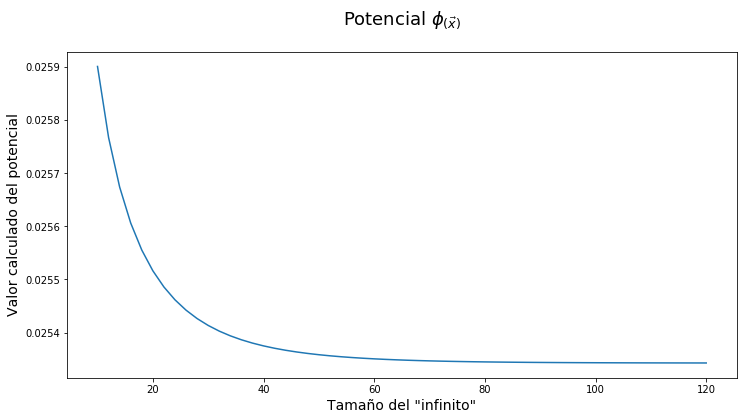
\includegraphics[width=\linewidth]{./Imagenes/phi_n.png}
%\caption{Convergencia del valor del potencial en función de $n$.}
%\end{figure}
%\noindent
%Se presenta también la diferencia porcentual entre los cálculos para distintos valores de $n$ en la Figura 6, con escala logarítmica en el eje de la variación para poder distinguir de mejor forma los cambios en el valor. Como ya se dijo y también como se puede ver en cualquiera de las dos gráficas, no merece la pena calcular para $n$ mucho mayores a 50, pues es poca la precisión que se gana, y para conjuntos de múltiples cargas se produce una demanda computacional innecesaria.\\\\
%Se puede observar que, teniendo en cuenta la escala logarítmica, la diferencia entre iteraciones después de la marca roja tiende a ser lineal, por lo que no se gana mucho aumentando el número de datos. Es para tener mayor certeza de la precisión del cálculo que se propone trabajar con $n = 70$. 
%\begin{figure}[H]
%\centering
%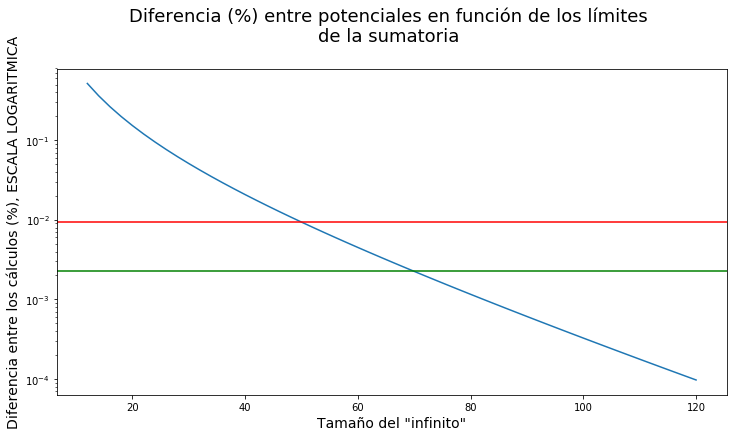
\includegraphics[width=\linewidth]{./Imagenes/delta_n.png}
%\caption{Variación porcentual del valor de $\phi$ en función de $n$.}
%\end{figure}
%




%%%%%%%%%%%%%%%%%%%%%%%%%%%%%%%%%%%%%%%%%%%%%%%%%%%%%

\subsection{El ciclo termodinámico en solvatación}
En el cálculo de energías de solvatación es muy útil analizar los estados en que se encuentra el sistema en cuestión. Para esto se realiza un ciclo termodinámico, que facilita el entendimiento de lo que se está calculando. En este trabajo se utiliza principalmente para entender justamente qué son los resultados que se estan obteniendo, y compararlos con el programa \texttt{APBSmem}.\\\\
Para el caso trabajado, el ciclo termodinámico común para \texttt{APBSmem} y \texttt{PyGBe} es el que se muestra en la figura \ref{fig:thermo_cycle} y que consiste de cuatro estados. El estado \circled{1} es el conjunto de cargas que componen la molécula y la membrana por separado en el vacío\footnote{Para efectos de ambos programas, el ``vacío" es en realidad un medio dieléctrico polarizable de permitividad igual a la de la molécula.}; como la membrana es un dieléctrico que no posee cargas explícitas, no hay una energía electrostática asociada, y para el caso del conjunto de cargas, la energía es simplemente la de Coulomb en el medio (Ec. (\ref{eqn:potential})). El estado \circled{2} corresponde a la membrana y el conjunto de cargas, nuevamente por separado, pero esta vez en agua en vez de en el vacío. La proteina y la membrana mantienen sus permitividades, por lo que en este caso hay una condición de salto en el borde de la proteina (Ec. (\ref{eqn:jump_condition})). El estado \circled{3} es un sistema en que la molécula esta embebida en la membrana, y este conjunto esta a su vez en el vacío, por lo que las constantes dieléctricas de la molécula y del vacío son las mismas. Finalmente, el estado \circled{4} es semejante al estado \circled{3}, pero por fuera del conjunto membrana-proteina hay agua con su respectiva permitividad. Las diferencias energéticas de la \circled{A} a la \circled{E} se detallan a continuación.
\begin{table}[H]\label{table:thermo_cycle_details}
	\centering
	\caption{Expresión de las diferencias energéticas, en función de los estados 1 a 4. $\Delta G$ es la diferencia en la energía libre de Gibbs entre los distintos estados del ciclo \ref{fig:thermo_cycle}.}
	\setlength{\tabcolsep}{30pt}
	\begin{tabular}{cc}
		\circled{A} & $\Delta G_{\circled{2} - \circled{1}}$ \\
		\circled{B} & $\Delta G_{\circled{3} - \circled{1}}$ \\
		\circled{C} & $\Delta G_{\circled{4} - \circled{2}}$ \\
		\circled{D} & $\Delta G_{\circled{4} - \circled{3}}$ \\
		\circled{E} & $\Delta G_{\circled{4} - \circled{1}}$
	\end{tabular}
\end{table}
\noindent
Se debe resaltar que, como en cualquier ciclo termodinámico, un camino cerrado suma cero si se es consistente. Esta propiedad es sumamente importante, pues \texttt{PyGBe} solo puede calcular directamente diferencias de energías que involucren el estado \circled{1} en la figura \ref{fig:thermo_cycle}; gracias a que un camino cerrado da cero, se pueden calcular las diferencias de energía faltantes - en este caso \circled{C} y \circled{D} - a partir del resto del ciclo.
\begin{figure}[H]
	\centering
	\input{./Figures/Fig_9.eps_tex}
	\caption{Ciclo termodinámico estudiado según lo presentado en los párrafos anteriores. Lo que se calcula principalmente entre \texttt{PyGBe} y \texttt{APBS} es la diferencia}% \circled{E}.}
	\label{fig:thermo_cycle}
\end{figure}




%%%%%%%%%%%%%%%%%%%%%%%%%%%%%%%%%%%%%%%%%%%%%%%%%%%%%



\chapter{Resultados}
En primer lugar se recuerda que la meta de todo este trabajo es simular energías de solvatación de proteínas embebidas en membranas, analizando tres casos simples y contrastando resultados con un programa ampliamente aceptado y usado (APBS y APBSmem), tanto en términos de precisión del cálculo como en tiempo de cómputo requerido. Los tres casos simples son un ion de carga unitaria, un arreglo de tres iones, también individualmente de carga unitaria, uno de ellos de radio tal que encierra a los otros, y el tercer caso es una molécula de bromoetano (Anexo).
\section{Cálculo numérico de las energías}
Las pruebas se realizaron con una membrana de espesor $a = 20 \angstrom$, con una de las dos interfaces ubicada en el plano $z=-10 \angstrom$ respecto del origen $(0,0,0)$ en coordenadas cartesianas.\\\\%Las permitividades se presentan en la Tabla 1, a continuación
%\begin{table}[H]
%\setlength{\tabcolsep}{32pt}
%\centering
%\caption{Permitividades de los tres medios trabajados}
%\begin{tabular}{ccc}\hline
%$\varepsilon_m = 2$ & $\varepsilon_p = 4$ & $\varepsilon_w = 80$\\\hline
%\end{tabular}
%\end{table}
%\noindent
Las permitividades están adimensionalizadas, su valor siendo el descrito en el apartado \ref{subsec:Macro_perm}. Los subíndices son, respectivamente de izquierda a derecha, indicadores de \textit{membrane (membrana)}, \textit{protein (proteína)} y \textit{water (agua)}.\\\\
Los cálculos se realizan para tres densidades de malla, para los tres casos de prueba, y para los dos programas - PyGBe y APBSmem. Los cálculos realizados corresponden a la diferencia \circled{4} - \circled{1} en el ciclo termodinámico \ref{fig:thermo_cycle}, con las siguientes propiedades

\begin{table}[H]
	\setlength{\tabcolsep}{32pt}
	\centering
	\caption{Permitividades en los estados de interés}
	\begin{tabular}{cccc}\hline
		Estado & $\varepsilon_m$ & $\varepsilon_p$ & $\varepsilon_w$\\\hline
		\circled{1} & - & 4.0 & 4.0 \\
		\circled{4} & 2.0 & 4.0 & 80.0
	\end{tabular}
\end{table}

\subsection{Resultados mediante PyGBe}
Para calcular las energías de solvatación con PyGBe, se utiliza \texttt{MSMS} para generar las mallas en archivos de formato \texttt{.vert} y \texttt{.face}, como se explica en la sección \ref{Sec:SW_Description}. Se crean tres mallas por caso de estudio; la densidad de elementos se aumenta a una tasa constante para poder realizar un análisis mediante extrapolación de Richardson, como se presenta más adelante. Los casos estudiados son \texttt{centered\_ion}, \texttt{3q} y \texttt{bromoethane}. El primer caso es un único ion en (0,0,0) de radio $1\,\angstrom$, el segundo son 3 iones, uno de radio $4\,\angstrom$ en (0,0,0) y los otros de radio $1\,\angstrom$ ubicados completamente dentro del volumen del primer ion, y el tercer caso es una molécula de 8 átomos con diversos radios y cargas. Las densidades de elementos de borde utilizadas, en $\frac{vert}{\angstrom^2}$, son 2, 4 y 8.\\\\
Para calcular los siguientes resultados se utilizaron 3 puntos de cuadratura para elementos lejanos, 37 en los paneles cercanos, y 9 puntos para el semianalítico. Además, el número de imágenes se mantuvo constante en $N=41$ para estas pruebas; más adelante se presenta un análisis en función de variar el parámetro $N$ para ver cómo es la convergencia y mostrar que con 41 imágenes es suficiente.
Sobre el primer caso, \texttt{centered\_ion}, se presentan a continuación los resultados obtenidos para las 3 mallas, junto con los tiempos de cálculo totales.

\begin{table}[H]
	\centering
	\caption{}
	\def\arraystretch{0.8}
	\begin{tabular}{cccccc}\hline
		\multirow{2}{*}{Densidad} & Número de & \multirow{2}{*}{E\_solv (PyGBe)} & E\_solv (PyGBe & Tiempo de & RAM\\
		 & elementos &  & + Membrana) & cálculo & utilizada\\\hline
		vert.$/\angstrom^2$ & \rule{0pt}{15pt}[-] & kcal/mol & kcal/mol & [s] & [GB] \\\hline
		d02 & 736 & -9.919124 & 5.258441 & 45.146 & 3.6\\
		d04 & 1572 & -9.886872 & 5.243907 & 176.890 & 15.9\\
		d08 & 3124 & -9.872508 & 5.236550 & 696.899 & 63.9
	\end{tabular}\label{table:pygbe_centered_ion}
\end{table}
\noindent
Para el segundo caso, \texttt{3q}, las energías son mayores, por lo que como se ve más adelante, el error relativo es bastante menor que en el caso anterior (\texttt{centered\_ion}) y el que se ve después (\texttt{bromoethane}). A continuación se presenta una tabla equivalente a la anterior, pero en este caso solo se presentan las energías, pues los tiempos y la memoria consumidos varían muy poco, ya que la discretización de la superficie es la misma que en el caso anterior.

\begin{table}[H]
	\centering
	\caption{}
	\def\arraystretch{0.8}
	\begin{tabular}{cccc}\hline
		\multirow{2}{*}{Densidad} & Número de & \multirow{2}{*}{E\_solv (PyGBe)} & E\_solv (PyGBe \\
		& elementos &  & + Membrana) \\\hline
		\rule{0pt}{15pt} vert.$/\angstrom^2$ & [-] & kcal/mol & kcal/mol \\\hline
		d02 & 736 & -90.703972 & 47.973011 \\
		d04 & 1572 & -90.391445 & 47.841024 \\
		d08 & 3124 & -90.252742 & 47.774469
	\end{tabular}\label{table:pygbe_3q}
\end{table}
\noindent
Finalmente, para la molécula de bromoetano se presenta nuevamente una tabla como la \ref{table:pygbe_centered_ion}, pues la geometría en este caso es distinta a una esfera y se debió mapear la superficie. La molécula tiene un área menor, lo que se traduce en un tiempo de cálculo y consumo de memoria menores para la misma densidad de elementos. Para este caso se omite la extrapolación de Richardson debido a que los resultados de los cálculos no están en sucesión creciente o decreciente, por lo que dicho método de extrapolación no es aplicable. La tabla de resultados en cuestión es la siguiente:

\begin{table}[H]
	\centering
	\caption{}
	\def\arraystretch{0.8}
	\begin{tabular}{cccccc}\hline
		\multirow{2}{*}{Densidad} & Número de & \multirow{2}{*}{E\_solv (PyGBe)} & E\_solv (PyGBe & Tiempo de & RAM\\
		& elementos &  & + Membrana) & cálculo & utilizada\\\hline
		\rule{0pt}{15pt} vert.$/\angstrom^2$ & [-] & kcal/mol & kcal/mol & [s] & [GB] \\\hline
		d02 & 322 & -0.348698 & 0.218434 & 17.852 & 1.0\\
		d04 & 694 & -0.339504 & 0.221408 & 60.248 & 4.1\\
		d08 & 1448 & -0.339504 & 0.220199 & 224.459 & 19.2
	\end{tabular}\label{table:pygbe_bromoethane}
\end{table}


\subsection{Resultados mediante APBS - APBSmem}

Para poder validar los resultados obtenidos con \texttt{PyGBe} se requiere una referencia contra la cual comparar. El software \texttt{APBSmem} se utiliza para este propósito, en vista de su renombre. Ahora bien, como el programa lo que hace es parcelar una "caja`` (el dominio de integración) nodos en los que calcula, dependiendo de las condiciones en dicho nodo, la ecuación gobernante correspondiente, se requieren setear condiciones en los bordes de la mencionada caja. \texttt{APBSmem}, al igual que \texttt{APBS}, permite establecer dichas condiciones. Para el caso trabajado existen tres, que son explicados en el apartado \ref{subsec:APBS}. Se presentan por ende tres tablas para el caso del archivo \texttt{centered\_ion}, dos para el caso \texttt{3q} (se explica el por qué al presentar los resultados), y el valor de evaluación más fino para la molécula de \texttt{bromoethane}, en vista que no se puede extrapolar un resultado con PyGBe.\\\\
Como en \texttt{APBSmem} hay que definir un dominio de integración rectangular, se opta por un cubo de $128\,\angstrom$ de lado, con tres cantidades de elementos, de modo que cada uno de estos sea de $0.25\,\angstrom, 0.5\,\angstrom$ y $1\,\angstrom$. Se utiliza \texttt{APBS} con mapas dieléctricos modificados para incluir la membrana, y el programa entrega la misma diferencia que \texttt{PyGBE}, pero en unidades de $kJ/mol$. Esto no requiere más que una división por $4.184\, kJ/kcal$ para hacer los resultados directamente comparables. Siguiendo el mismo orden que para \texttt{PyGBe}, los resultados para el primer caso de estudio son los siguientes

\begin{table}[H]
	\centering
	\caption{}
	\def\arraystretch{0.8}
	\begin{tabular}{|ccccccc|}\hline
		Tipo de & \multirow{2}{*}{$\Delta$x} & Número de & \multirow{2}{*}{E\_solv} & \multirow{2}{*}{E\_solv} & Tiempo de & RAM\\
		condición &  & elementos &  &  & cálculo & utilizada\\\hline
		&  $\angstrom$ & [-] & kJ/mol & kcal/mol & [s] & [GB] \\\hline
		\parbox[t]{2mm}{\multirow{3}{*}{\rotatebox[origin=c]{90}{\texttt{zero}}}} & 1.00 & 128 & 22.65401 & 5.41420 & 16.548 & 0.5\\
		& 0.50 & 256 & 22.46140 & 5.36840 & 131.126 & 3.8\\
		& 0.25 & 512 & 22.30540 & 5.33112 & 1208.873 & 29.7\\ \hline
		\parbox[t]{2mm}{\multirow{3}{*}{\rotatebox[origin=c]{90}{\texttt{sdh}}}} & 1.00 & 128 & 20.39885 & 4.87544 & 16.872 & 0.5\\
		& 0.50 & 256 & 20.20733 & 4.82967 & 132.265 & 3.8\\
		& 0.25 & 512 & 20.05135 & 4.79239 & 1150.529 & 29.7\\ \hline
		\parbox[t]{2mm}{\multirow{3}{*}{\rotatebox[origin=c]{90}{\texttt{mdh}}}} & 1.00 & 128 & 20.39885 & 4.87544 & 16.361 & 0.5\\
		& 0.50 & 256 & 20.20733 & 4.82967 & 134.597 & 3.8\\
		& 0.25 & 512 & 20.05135 & 4.79239 & 1226.290 & 30.8\\ \hline
	\end{tabular}\label{table:apbs_centered_ion}
\end{table}

A continuación se muestran los resultados para \texttt{3q}, y la razón de solo presentar dos sets de resultados para esta molécula es que se repite el comportamiento apreciado en la tabla anterior, \ref{table:apbs_centered_ion}; las energías de solvatación para las condiciones \texttt{sdh} y \texttt{mdh} no varían, probablemente porque los casos de estudio son muy simples. Por esto es que únicamente se presentan los datos correspondientes a condiciones de contorno \texttt{zero} y \texttt{sdh}.

\begin{table}[H]
	\centering
	\caption{}
	\def\arraystretch{0.8}
	\begin{tabular}{|ccccccc|}\hline
		Tipo de & \multirow{2}{*}{$\Delta$x} & Número de & \multirow{2}{*}{E\_solv} & \multirow{2}{*}{E\_solv} & Tiempo de & RAM\\
		condición &  & elementos &  &  & cálculo & utilizada\\\hline
		&  $\angstrom$ & [-] & kJ/mol & kcal/mol & [s] & [GB] \\\hline
		\parbox[t]{2mm}{\multirow{3}{*}{\rotatebox[origin=c]{90}{\texttt{zero}}}} & 1.00 & 128 & 207.06438 & 49.48957 & 0.6 & 23.602 \\
		& 0.50 & 256 & 204.90048 & 48.97239 & 4.0 & 137.004 \\
		& 0.25 & 512 & 203.40408 & 48.61474 & 29.9 & 1174.478 \\ \hline
		\parbox[t]{2mm}{\multirow{3}{*}{\rotatebox[origin=c]{90}{\texttt{sdh}}}} & 1.00 & 128 & 186.77688 & 44.64074 & 0.6 & 23.958 \\
		& 0.50 & 256 & 184.61382 & 44.12376 & 3.9 & 127.519 \\
		& 0.25 & 512 & 183.11772 & 43.76619 & 29.9 & 1093.347 \\ \hline
	\end{tabular}\label{table:apbs_3q}
\end{table}

Para el caso de la molécula de bromoetano se presenta simplemente el valor más fino calculado en \texttt{APBSmem}; esto para condiciones \texttt{zero} y \texttt{sdh}.

\begin{table}[H]
	\centering
	\caption{}
	\def\arraystretch{0.8}
	\begin{tabular}{|ccccccc|}\hline
		Tipo de & \multirow{2}{*}{$\Delta$x} & Número de & \multirow{2}{*}{E\_solv} & \multirow{2}{*}{E\_solv} & Tiempo de & RAM\\
		condición &  & elementos &  &  & cálculo & utilizada\\\hline
		&  $\angstrom$ & [-] & kJ/mol & kcal/mol & [s] & [GB] \\\hline
	\texttt{zero} & 0.25 & 512 & 0.90307 & 0.21584 & 1194.226 & 30.8 \\
	\texttt{sdh} & 0.25 & 512 & 0.90299 & 0.21582 & 1206.741 & 29.7 \\ \hline
	\end{tabular}\label{table:apbs_brom}
\end{table}

\section{Extrapolación de Richardson y error relativo}
Para poder comprobar de manera fehaciente que utilizar el método de imágenes acoplado a \texttt{PyGBe} es un método válido de simular una proteína embebida en una membrana, se utiliza una extrapolación de Richardson para comparar los cálculos. La extrapolación de Richardson es una herramienta que permite, como indica el nombre, realizar una extrapolación mediantes tres puntos para obtener el valor ``límite" teórico al que se llegaría si la malla se afinara consecutivamente a una tasa constante. Es por esta razón que todos los cálculos realizados previamente presentan una razón de densificación constante. La fórmula para obtener el resultado teórico extrapolado es
\begin{equation}
G_t = \frac{G_1\cdot G_3 - (G_2)^2}{G_1 - 2G_2 + G_3}
\end{equation}
Para esto se debe cumplir que $G_2:G_1 = G_3:G_2$. Con este método aclarado es que se presentan los resultados extrapolados para cada uno de los dos casos de estudio (\texttt{centered\_ion} y \texttt{3q}), así como también una comparación porcentual entre los resultados extrapolados obtenidos mediante \texttt{PyGBe} y \texttt{APBS - APBSmem}. Para el caso de \texttt{bromoethane} se calcula una diferencia porcentual entre los resultados para las mallas más finas solamente. Como \texttt{APBSmem} tiene dos resultados distintos (tres en realidad, pero se utilizan solo \texttt{zero} y \texttt{sdh} por los motivos explicados previamente) dependiendo de las condiciones de contorno utilizadas, se presentan dos errores porcentuales; sin embargo, se adelanta que el menor error corresponde a la condición de borde \texttt{zero} todos los casos estudiados. La razón principal que provoca esto, por lo que se infiere, se desarrolla en la sección de análisis de los resultados obtenidos.



%En la sección actual se presentan una serie de breves resúmenes de publicaciones relacionadas con la temática de modelos computacionales de células y/o biomoléculas, o que sean de aporte para el entendimiento de la teoría electrostática en alguna forma.
%\subsection{APBSmem: A Graphical Interface for Electrostatic Calculations at the Membrane \cite{APBSmem}}
%La publicación sobre APBSmem es más que nada una guía para la utilización del programa APBSmem, en la que se presentan además los métodos utilizados para el cálculo de energías de interés, en sistemas biológicos (proteína-membrana principalmente); esto puede ser, solvatación para iones, para proteínas, o canales transmembrana. 
%La bicapa consiste en ``planchas" de material dieléctrico con baja constante dieléctrica que se colocan de tal forma que limiten con la proteína y no sean parte de, en el caso que haya, las proteínas de canal. Para ubicar la membrana, el programa utiliza las posiciones espaciales de residuos hidrofóbicos como referencia, o también se puede acudir a la base de datos Orientations of Proteins in Membranes.\\\\
%Utilizando la ecuación PB lineal, el programa puede calcular el potencial de membrana o proteína por separado, en caso que sea requerido. Se incluyen las ecuaciones de PB para tres casos: bajo la membrana (dentro de la célula), en la membrana, y sobre esta (fuera de la célula). Esto se logra con la ecuación de Poisson-Boltzman linealizada y sumando un término para compensar por la diferencia de potencial entre el interior y el exterior; esta diferencia es producto de la concentración de iones (Potasio, Calcio, etc) al interior y exterior de la pared celular. Los potenciales del sistema vienen de la ecuación PB por fuera de la célula, PB modificado para dar cuenta de la concentración de iones dentro de la célula, y Poisson (Laplace) dentro en la membrana; para una bicapa con límites $z = L/2$ y $z = -L/2$, los potenciales son
%
%\begin{align}
%\phi_1(z) &= \frac{e}{k_BT}V_{in}\frac{1}{\frac{\epsilon_w}{\epsilon_m}\kappa L + 2}e^{\kappa(L/2 - z)} &z>L/2\\
%\phi_2(z) &= \frac{e}{k_BT}V_{in}\left(\frac{1}{2}-\frac{1}{\frac{\epsilon_w}{\epsilon_m}\kappa L + 2}\frac{\epsilon_w}{\epsilon_m}\kappa z\right) &-L/2 < z < L/2\\
%\arraycolsep=0.3in\def\arraystretch{2}
%\phi_3(z) &= \frac{e}{k_BT}V_{in}\left(1 - \frac{1}{\frac{\epsilon_w}{\epsilon_m}\kappa L + 2}e^{\kappa(z+ L/2)}\right)&z<-L/2
%\end{align}
%En este caso $\phi_{1,2,3}$ es el potencial producto de la membrana, $e$ es la carga del electrón, y $\kappa^2=\bar{\kappa}^2/\epsilon_w$ es una variable auxiliar relacionada con la longitud de Debye-Hückel $\bar{\kappa}$.\\\\
%El programa, según se escribe en la publicación, trabaja con el método de diferencias finitas para obtener el potencial. Se incluyen ejemplos para los tres casos de cálculos energéticos mencionados en el paper.
%\subsection{Image Approximations to Electrostatic Potentials in Layered Electrolytes/Dielectrics and an Ion-Channel Model.\cite{Huimin-Lin}}
%En esta publicación se estudia la ecuación de PB linealizada aproximada mediante el método de imágenes; en particular, se modela el campo de reacción del solvente y la membrana en presencia de un canal iónico. Para esto, los investigadores obtienen imágenes para las interfaces planas de la membrana y para una interfaz propia de un cilindro, que sirve para separar al canal iónico del resto del sistema estudiado. Se determina una aproximación por el método de imágenes dentro y fuera de la membrana y del cilindro. Se integran también los aportes iónicos de la solución al modelo, lo que genera una expansión en funciones ortogonales de $sin$ y $cos$ para el potencial de Coulomb y el campo de reacción en la membrana. De la publicación se tienen las expresiones para el potencial en la membrana, sobre ella y bajo ella en $z$. Además, las imágenes y sus posiciones se obtienen por uno de dos métodos. El primero es una solución de la minimización del error $L_2$ entre la expresión propuesta por el método RIC \cite{Pei-kun} y el método de múltiples imágenes, que presenta Wei Cai en otro paper \cite{Wei-Cai}.
%\begin{align*}
%\text{Sol. RIC}\qquad\qquad \phi_{rf} = &\sum_{\substack{k = -\infty\\
%k \neq 0}}^{k = \infty} \frac{q_k}{\epsilon_m|\vec{x} - \vec{x}_k|}\\
%\text{Sol. Mult. Im. Method}\qquad\qquad \phi_{irf} = & \frac{q_s}{\epsilon_m}\sum_{l}\frac{q_k}{|\vec{x} - \vec{x}_l|}
%\end{align*}
%La segunda alternativa es utilizar un método de ajuste tipo Prony para resolver el sistema, aplicando dicho ajuste a la expansión de Fourier. En el paper se menciona que no existe actualmente una forma de modelar los efectos de la solución electrolítica sobre el canal iónico mediante el método de imágenes. Para modelar el canal intermembrana a pesar de este obstáculo es que se propone el uso de un modelo híbrido: se utiliza el método de imágenes para modelar los potenciales de la membrana y del solvente. Se utiliza un cilindro para encerrar el canal, junto con parte del solvente y la membrana, y se calculan las condiciones en las interfaces correspondientes al cilindro con el método de imágenes. Con esto se puede utilizar otro método, como dinámica molecular, para realizar los cálculos correspondientes al canal intermembrana a partir del borde del cilindro, cuyas condiciones son ya conocidas.
%\subsection{Multiple-image treatment of induced charges in Monte Carlo simulations of electrolytes near a spherical dielectric interface \cite{Gan}}
%Se emplea el método de imágenes para simular un coloide esférico, en primera instancia sin carga. El coloide se considera un macroión, sumergido en un dieléctrico en el que hay más especies iónicas distribuidas. Para esto se ocupa la ecuación de Poisson para el potencial, que surge de aplicar $\nabla$ a la ecuación (7). Se tratan los iones del solvente como cargas puntuales, considerando de inmediato una formulación explícita del problema. Como el coloide no tiene carga, se trabaja con la ecuación de Laplace.\\\\
%Ahora, fuera del coloide esférico se tiene que
%\begin{equation*}
%\Phi(\vec{r}) = \Phi_{Coul}(\vec{r}) + \Phi_{pol}(\vec{r})
%\end{equation*}
%El potencial de polarización es el complejo en este problema, pues el de Coulomb es el ya conocido $q/(\epsilon|\vec{r}-\vec{r}_s|)$.\\\\
%Para el potencial de polarización se ubican cargas a lo largo de una recta, de tal forma que se genere la esfera para una carga $q$ real ubicada a una distancia $r_s$ del centro de referencia. Con una expansión harmónica, se puede reformular el potencial de polarización como las contribuciones de una carga $q_K = -\gamma a q/r_s$, llamada de Kelvin, y una distribución lineal de carga desde el origen hasta la posición de $q_K$. Esta se puede discretizar y llevar a una sumatoria de la forma
%\begin{gather*}
%\Phi_{pol}(\vec{r}) = \frac{q_K}{\epsilon|\vec{r} - \vec{r}_K} + \sum_{m = 1}^I \frac{q_m}{\epsilon|\vec{r} - \vec{x}_m|}\\
%q_m = \frac{\omega_m}{2}\frac{\gamma a q}{r_s}\qquad\qquad x_m = r_K\left(\frac{1-s_m}{2}\right)^{1/\sigma}
%\end{gather*}
%donde $\gamma=(\epsilon_{in} - \epsilon_{out})/(\epsilon_{in}+ \epsilon_{out})$, $\sigma = \epsilon_{out}/(\epsilon_{in} + \epsilon_{out})$, $a$ el radio del coloide esférico, $r_K$ es el radio de la carga de Kelvin desde el centro del sistema de referencia, y $q$ es la carga de prueba. A partir de esto, se puede aproximar la carga lineal distribuida mediante $I + 1$ cargas puntuales. Establecido esto, se utiliza un método de Monte Carlo para el cálculo de la energía potencial del coloide en el dieléctrico.



%%%%%%%%%%%%%%%%%%%%%%%%%%%%%%%%%%%%%%%%%%%%%%%%%%%%%


\chapter{Conclusiones}
Durante el aprendizaje que conlleva el presente trabajo se logra afianzar el conocimiento sobre la teoría electrostática, así como también familiarizarse con la ecuación de Poisson-Boltzman (a través de las lecturas pertinentes al tema), de dónde surge y todo lo que representa. Ya se señaló en un principio que la idea principal de este escrito es presentar la base teórica para poder implementar BEM, y en primera instancia eso se logra para un medio homogeneo, pues ya se cuenta con una expresión para el potencial en función de las variables de interés del problema.\\\\
En este informe se aclara por qué es posible utilizar la teoría electrostática macroscópica para describir fenómenos a nivel molecular, dando paso a la explicación y aplicación del método de imágenes para resolver un sistema simple de una carga y una interfaz planar. Con la introducción y resolución de la teoría y el problema tipo del método de imágenes respectivamente, se procede a la implementación del método RIC. Mediante esta última herramienta se pueden trabajar sistemas de múltiples cargas en un medio encerrado por dos interfaces a través de cargas imágenes que representen el campo de reacción de los medios. Gracias a un pequeño programa es que se logra definir un número conveniente para representar el valor de $\infty$ en los límites de la sumatoria para el caso de una sola carga encerrada.
\section{Continuación del trabajo}
A continuación se plantea cómo seguir con este trabajo a partir de los fundamentos establecidos en el presente texto, pues la idea es hacer uso de la teoría incluida aquí para entregar un aporte, particularmente buscando una mejora en la velocidad de cálculo.\\\\
Teniendo ya definida la temática y la materia cubierta en este informe, lo que queda es hacer uso de la teoría de una forma útil y eficiente. En la sección introductoria se mencionó el método de elementos de borde BEM. Pues bien, para dar continuidad a esta línea de investigación, se busca implementar dicho método a un sistema como el visto en el apartado 3.\\\\
El objetivo ideal que se plantea es establecer una forma de modelar computacionalmente una representación de una proteina sometida a interacciones electrostáticas mientras está inserta en la membrana, y en determinar también si el aporte de dicha membrana es realmente significativo o se puede despreciar, y en qué casos es correcto hacerlo.\\\\
También hay otros puntos de investigación, como simular una o un sistema de cargas fuera de la membrana. Esto abriría la posibilidad de trabajar con proteínas transmembrana sin tener que cambiar de forma significativa el planteamiento del problema. Además puede ser que si se continúa con esta línea de investigación, surjan otras aristas que valga la pena explorar y sean de interés.\\\\
Cerrando las ideas, se puede decir que el trabajo presentado en este informe consiste en adquirir conocimientos base e información sobre otros trabajos relacionados con el tema. Esto se hace para poder avanzar en lo sucesivo con el desarrollo de nuevas propuestas que permitan acelerar los cálculos energéticos de la interacción electrostática en sistemas de múltiples cargas. Queda pendiente familiarizarse con el método BEM, para poder así juntar todo en un trabajo final que englobe la teoría electrostática aplicada a interacciones moleculares de proteínas en la membrana mediante el método de elementos de borde.


\pagebreak

\begin{thebibliography}{20}
\bibitem{Jackson}
Jackson, J. D. \textit{Classical Electrodynamics}, Third Edition; Wiley, 1998
\bibitem{Griffiths}
Griffiths, D. J. \textit{Introduction to Electrodynamics}, Third Edition; Prentice Hall, 1999
\bibitem{Kantorovich}
Kantorovich, L. \textit{Quantum Theory of the Solid State: An Introduction}, First Edition; Springer, 2004
\bibitem{Cai}
Cai, W. \textit{Computational Methods for Electromagnetic Phenomena}, First Edition; Cambridge University Press, 2013
\bibitem{Brebbia}
Brebbia, C. A.; Dominguez J. \textit{Boundary Elements: An Introductory Course}, Second Edition; WIT Press, 1992
\bibitem{Cooper2015}
Cooper, C. \textit{Biomolecular Electrostatics With Continuum Models: A Boundary Integral Implementation and Applications to Biosensors}, 2015
\bibitem{Pei-kun}
Yang, P.; Liaw, S.; Lim, C. \textit{Representing an Infinite Solvent System with a Rectangular Finite System Using Image Charges}, J. Phys. Chem. B 2002, 106, 2973-2982
\bibitem{APBSmem}
Callenberg, K. M.; Choudhary, O. P.; de Forest, G. L.; Gohara, D. W.; Baker, N. A.; Grabe, M. \textit{APBSmem: A Graphical Interface for Electrostatic Calculations at the Membrane}, PLoS ONE 5(9), 2010
\bibitem{Huimin-Lin}
Lin, H.; Xu, Z.; Tang, H.; Cai, W. \textit{Image Approximations to Electrostatic Potentials in Layered Electrolytes/Dielectrics and an Ion-Channel Model}, J. Sci. Comput., 2011
\bibitem{Wei-Cai}
Cai, W.; Deng, S.; Jacobs, D. \textit{Extending the fast multipole method to charges inside or outside a dielectric sphere} J. Comput. Phys. 223, 2007
\bibitem{Gan}
Gan, Z.; Xu, Z. \textit{Multiple-image treatment of induced charges in Monte Carlo simulations of electrolytes near a spherical dielectric interface} Phys. Rev. E 84, 016705, 2011
\bibitem{Roux}
Roux, B. \textit{Influence of the Membrane Potential on the Free Energy of an Intrinsic Protein} Byophysical Journal, Vol. 73, 2980-2989, 1997
\bibitem{Campbell}
Campbell, N.; Reece, J. \textit{Biología}, Séptima Edición, Editorial Médica Panamericana, 2007
\bibitem{Lombard}
Lombard, J. \textit{Once upon a time the cell membranes: 175 years of cell boundary research} Biology Direct 9:32, 2014
\bibitem{Zhu}
Zhenhai, Z.; Jingfang, H.; Song, B.; White, J. \textit{Improving the Robustness of a Surface Integral Formulation for Wideband Impedance Extraction of 3D Structures} IEEE/ACM International Conference on Computer Aided Design. 592-597, 2001 
\bibitem{Durand}
Durand, E. \textit{Électrostatique Vol. III Méthodes de Calcul Diélectriques} Masson et Cie.; 1966
\end{thebibliography}

%\pagebreak

%\section*{Anexos}

\end{document}